\documentclass[notitlepage,11pt, a4paper]{article}
\usepackage[utf8]{inputenc}

\usepackage{amsfonts, amssymb, amsmath}
\usepackage{mathtools}
\usepackage{fullwidth}
\usepackage{graphicx}

\usepackage{bm} % for bolding accents

\usepackage{caption}
\usepackage{subcaption}

\usepackage{algorithm2e}

\usepackage[colorlinks=true, pdfstartview=FitV, linkcolor=blue, citecolor=blue, urlcolor=blue,pagebackref=false]{hyperref}
\usepackage{varioref}
\usepackage[capitalize]{cleveref}

\usepackage[title]{appendix}


% BIBLIOGRAPHY MANAGEMENT

\usepackage[numbers]{natbib}
\bibliographystyle{plainnat}

% PAGE DIMENSIONS

\topmargin -0.5in
\textheight 9 in
\oddsidemargin 0.15in
\evensidemargin 0.25in
\textwidth 6.15in
\parskip=5pt

% THEOREM ENVIRONMENTS

\usepackage{amsthm}
\usepackage{thmtools, thm-restate}

\declaretheorem[numberwithin=section]{theorem}
\declaretheorem[sibling=theorem]{lemma}
\declaretheorem[sibling=theorem]{corollary}
\declaretheorem[sibling=theorem]{proposition}
\declaretheorem[sibling=theorem]{remark}
\declaretheorem[sibling=theorem]{definition}
\renewcommand{\figurename}{\bf{Fig.}}

% COMMENT ENVIRONMENTS

\usepackage{xcolor}
\definecolor{darkred}{rgb}{0.9,0.1,0.1}
\newcommand\comment[1]{\marginpar{\raggedright\scriptsize{\textcolor{darkred}{#1}}}}
\newcommand\myworries[1]{\textcolor{red}{[#1]}}

% ABBREVIATIONS

%%%%%%%%%% ABBREVIATIONS

% BLACKBOARD BOLD

\def \C {{\mathbb C}}
\def \D {{\mathbb D}}
\def \E {{\mathbb E}}
\def \N {{\mathbb N}}
\def \P {{\mathbb P}}
\def \Q {{\mathbb Q}}
\def \R {{\mathbb R}}
\def \Z {{\mathbb Z}}
\def \T {{\mathbb T}}
\def \I {{\mathbb I}}
\def \T {{\mathbb T}}

% MATHCAL

\def \cA {{\mathcal A}}
\def \cC {{\mathcal C}}
\def \cD {{\mathcal D}}
\def \cE {{\mathcal E}}
\def \cF {{\mathcal F}}
\def \cG {{\mathcal G}}
\def \cH {{\mathcal H}}
\def \cI {{\mathcal I}}
\def \cJ {{\mathcal J}}
\def \cK {{\mathcal K}}
\def \cL {{\mathcal L}}
\def \cM {{\mathcal M}}
\def \cN {{\mathcal N}}
\def \cO {{\mathcal O}}
\def \cP {{\mathcal P}}
\def \cQ {{\mathcal Q}}
\def \cR {{\mathcal R}}
\def \cS {{\mathcal S}}
\def \cT {{\mathcal T}}

% VECTORS

\def \vD {{\mathbf D}}
\def \vX {{\mathbf X}}
\def \vZ {{\mathbf Z}}
\def \va {{\mathbf a}}
\def \vc {{\mathbf c}}
\def \vd {{\mathbf d}}
\def \vk {{\mathbf k}}
\def \vs {{\mathbf s}}
\def \vu {{\mathbf u}}
\def \vx {{\mathbf x}}
\def \vy {{\mathbf y}}

% MAKING SUBSET AND SUPSET BY DEFAULT SUBSETEQ AND SUPSETEQ

\def \subset {\subseteq}
\def \supset {\supseteq}

% PAIRED DELIMITERS

\DeclarePairedDelimiter{\abs}{\lvert}{\rvert}
\DeclarePairedDelimiter{\norm}{\lVert}{\rVert}
\DeclarePairedDelimiter{\floor}{\lfloor}{\rfloor}

% MATH OPERATORS

\DeclareMathOperator{\var}{Var}
\DeclareMathOperator{\cov}{Cov}
\DeclareMathOperator{\corr}{Corr}
\DeclareMathOperator{\iso}{Iso}

% MISC SYMBOLS

\def\one{\rlap{\mbox{\small\rm 1}}\kern.15em 1} % indicator function

% CONVERGENCE
\def \todist {\xrightarrow[]{\mathrm{(d)}}}
\def \toas {\xrightarrow[]{\mathrm{a.s.}}}

% PROJECT SPECIFIC SYMBOLS

\usepackage{stmaryrd} % needed for double square brackets
\DeclarePairedDelimiter{\pathbtw}{\llbracket}{\rrbracket}
\def \littleo {o}
\def \bigo {O}
\newcommand \diff[2] {\frac{\mathrm{d}#1}{\mathrm{d}#2}}
\newcommand*\dif{\mathop{}\!\mathrm{d}}
\def \lattice {\Lambda}
\newcommand \vectwo[2] {\begin{pmatrix} #1 \\ #2 \end{pmatrix}}
\def \omegaevent {\mathcal E}
\def \maxeval {{\lambda_{\text{max}}}}
\def \mineval {{\lambda_{\text{min}}}}
\def \centeredX {\hat{\vX}}
\def \distmdm {d_{\vec{G}}}
\def \kernel {\kappa}
\def \zeroloop {\mathfrak L}

\def \toprob {\xrightarrow[]{\mathrm{(p)}}}
\def \toas {\xrightarrow[]{\mathrm{a.s.}}}

%%%%%%%%%%%%%%

\title{Universality for the directed configuration model: metric space convergence of the strongly connected components at criticality}
\author{ \and Zheneng Xie}

\author{Serte Donderwinkel\thanks{\href{mailto:serte.donderwinkel@stats.ox.ac.uk}{serte.donderwinkel@stats.ox.ac.uk}, University of Oxford, Oxford, United Kingdom. ORCID iD: 0000-0001-8148-8631.} \and Zheneng Xie \thanks{\href{zheneng.xie@stats.ox.ac.uk}{zheneng.xie@stats.ox.ac.uk}, University of Oxford, Oxford, United Kingdom. ORCID iD: 0000-0002-7252-3631. This research has been supported by the EPSRC Centre for Doctoral Training in Mathematics of Random Systems: Analysis, Modelling and Simulation (EP/S023925/1).}}
\date{\today}

\begin{document}
\maketitle
\begin{abstract}
  We consider the strongly connected components (SCC) of a uniform directed graph on $n$ vertices with i.i.d. degree tuples distributed as $(D^-,D^+)$, with $\E[D^+]=\E[D^-]=\mu$. We condition on the total in-degree and total out-degree to be equal. A phase transition for the emergence of a giant strongly connected component, that contains a positive proportion of the vertices, is known to occur at the critical value $\E[D^-D^+]/\mu=1$. We study the model at this critical value, and additionally, require that $\E[(D^-)^i(D^+)^j]<\infty$ for all $i+j\leq 3$, and for $i=3$, $j=1$. We show that, under these conditions, the strongly connected components ranked by decreasing order of size and rescaled by $n^{-1/3}$, converge in distribution to a sequence of finite strongly connected directed multigraphs with edge lengths which are either $3$-regular or loops. The limit objects are in a $3$-parameter family, which contains the scaling limit of the SCC in the directed Erd\H{o}s-Renyi model at criticality as found in \cite{goldschmidtScalingLimitCritical2019}. This shows that the limit object is universal, and makes this the first universality result for directed graph models. Moreover, this is the first time result on the directed configuration model at criticality. As a trivial consequence, the largest strongly connected components at criticality contain $O(n^{1/3})$ vertices with high probability, and the diameter of the directed graph at criticality is $\Omega(n^{1/3})$ with high probability; two results that were previously unknown.  We use a metric on the space of such multigraphs in which two multigraphs are close if there are compatible isomorphisms between their vertex and edge sets which roughly preserves the edge lengths. We use the product topology on the sequence of multigraphs. Our method involves depth-first exploration of the directed graph, resulting in a spanning forest, of which we study the limit under rescaling.
\end{abstract}
% \tableofcontents

\section{Introduction}


\subsection{Overview}

Edges in real-world networks are often directed, such as links on the world wide web, follows on Twitter or disease transmission. When analysing networks a natural quantity to consider is are the degrees of nodes in the network.  In this paper we will consider sampling an i.i.d.\ sequence of in- and out-degrees. Conditional on the total in-degree being equal to the total out-degree, we will sample a uniform directed graph (digraph) with the given degree sequence. Results on such graphs provide insight into what additional structure a real-world network has beyond it's degree sequence.

When considering such models, previous work by \citet{cooperSizeLargestStrongly2004} shows that there is a phase transition in the directed connectivity of the graph. Below some threshold, each of the strongly connected components of the graph will contain a negligible proportion of vertices in the graph whereas above the threshold there will exist a unique strongly connected component that occupies a positive proportion of the vertices.  We will study the behaviour of the model at criticality, specifically that there exists a sequence of random weighted directed multigraphs that can be understood as the scaling limit of the strongly connected components when viewed in decreasing order of size.

\subsection{Graph theory}

\begin{figure}
    \centering
    \includegraphics[scale=0.6]{Content/Pictures/biggraph2.pdf}
    \caption{A directed graph on [17]. The strongly connected components have vertex sets $\{1,2,5,17\}$, $\{3,6,8,9,14,16\}$, $\{7,11\}$, $\{4\}$, $\{10\}$, $\{12\}$, $\{13\}$, and $\{15\}$. Source figure: \cite{goldschmidtScalingLimitCritical2019}}
    \label{fig.SCCs}
\end{figure}

There are two notions of connectivity when working with a directed graph - weak and strong connectivity. We will be working with the strong notation. We say a vertex $v$ leads to a vertex $w$ if there exists a directed path from $v$ to $w$ in the graph. We say $v$ is strongly connected to $w$ if $v$ leads to $w$ and $w$ leads to $v$. A graph is strongly connected if any pair of vertices in the graph are strongly connected. The relation is an equivalence relation. The digraphs induced by the equivalence classes of are referred to as the strongly connected components (SCCs).

\subsection{Description of the model}

We consider $n$ vertices, to each of which we assign an in-degree and an out-degree. The degree tuples are independent and identically distributed with law $\nu$. For each $i\in [n]$, let $\mathbf{D}_i=(D^-_i,D^+_i)$ be the in- and out-degree of vertex $i$. In order for a graph with this degree sequence to exist, we require that $\sum_{i=1}^n D^-_i=\sum_{i=1}^n D^+_i$, so we will condition on this event. Conditional on $(\mathbf{D}_1,\dots,\mathbf{D}_n)$, sample a uniform digraph with this degree sequence. Denote resulting random digraph by $\vec{G}_n(\nu)$. We are interested in the limit under scaling of the strongly connected components of $\vec{G}_n(\nu)$ as $n\to \infty$.

We require the degree distribution to satisfy the following properties.

\begin{enumerate}
    % \item $\E[(D^-) + D^+)^3] < \infty$
    \item $\E[(D^-)^i(D^+)^j]< \infty$ for $1 \leq i+j\leq 3$ and for $\{i,j\}=\{1,3\}$
    \item $\E[D^-] = \E[D^+]$.
    \item \myworries{lattice condition}
\end{enumerate}

The first condition is required to ensure the steps of a random walk used in the proof has finite variance and thus will convergence (under rescaling) to a Brownian motion.

The second condition and third condition makes sure the event $\{\sum_{i=1}^n D^-_i = \sum_{i=1}^n D^+_i\}$ is well behaved. The second condition ensures this is not a large deviation event and the third condition ensures this event has positive probability for all $n \geq 1$. 

\myworries{go over criticality condition}

We define the following parameters, that will determine the behaviour of the strongly connected components in the limit.
\begin{enumerate}
    \item $\mu:=\E[D^-]=\E[D^+]=\E[D^-D^+]$
    \item $\nu_-:=\frac{\E[(D^-)^2]-\mu}{\mu}$ 
    \item $\sigma_-:=\left(\frac{\mu\E[(D^-)^3]-\E[(D^-)^2]^2}{\mu^2}\right)^{1/2}$ 
    \item $\sigma_+:=\left(\frac{\E[D^-(D^+)^2]-\mu}{\mu}\right)^{1/2}$ 
    \item $\sigma_{-+}:=\frac{\E[(D^-)^2D^+]-\E[(D^-)^2]}{\mu}$ 
\end{enumerate}
% \begin{remark}
% Conditions \ref{cond.beta} and \ref{cond.gamma} ensure that the Central Limit Theorem applies to the fluctuations of the first explored in-degrees around their mean. Condition \ref{cond.critical} ensures that the branching process corresponding to the depth-first exploration (i.e. the exploration of the out-components) is critical. Condition \ref{cond.rho} ensures that this branching process has Brownian scaling. Condition \ref{cond.tau} ensures that the covariance of the in- and out-degrees that are discovered first is finite. Condition \ref{cond.iota} ensures that the strongly connected components are $3$-regular. 
% \end{remark}
\subsection{Metric directed multigraphs and kernels}

\begin{figure}[htbp]
    \centering

    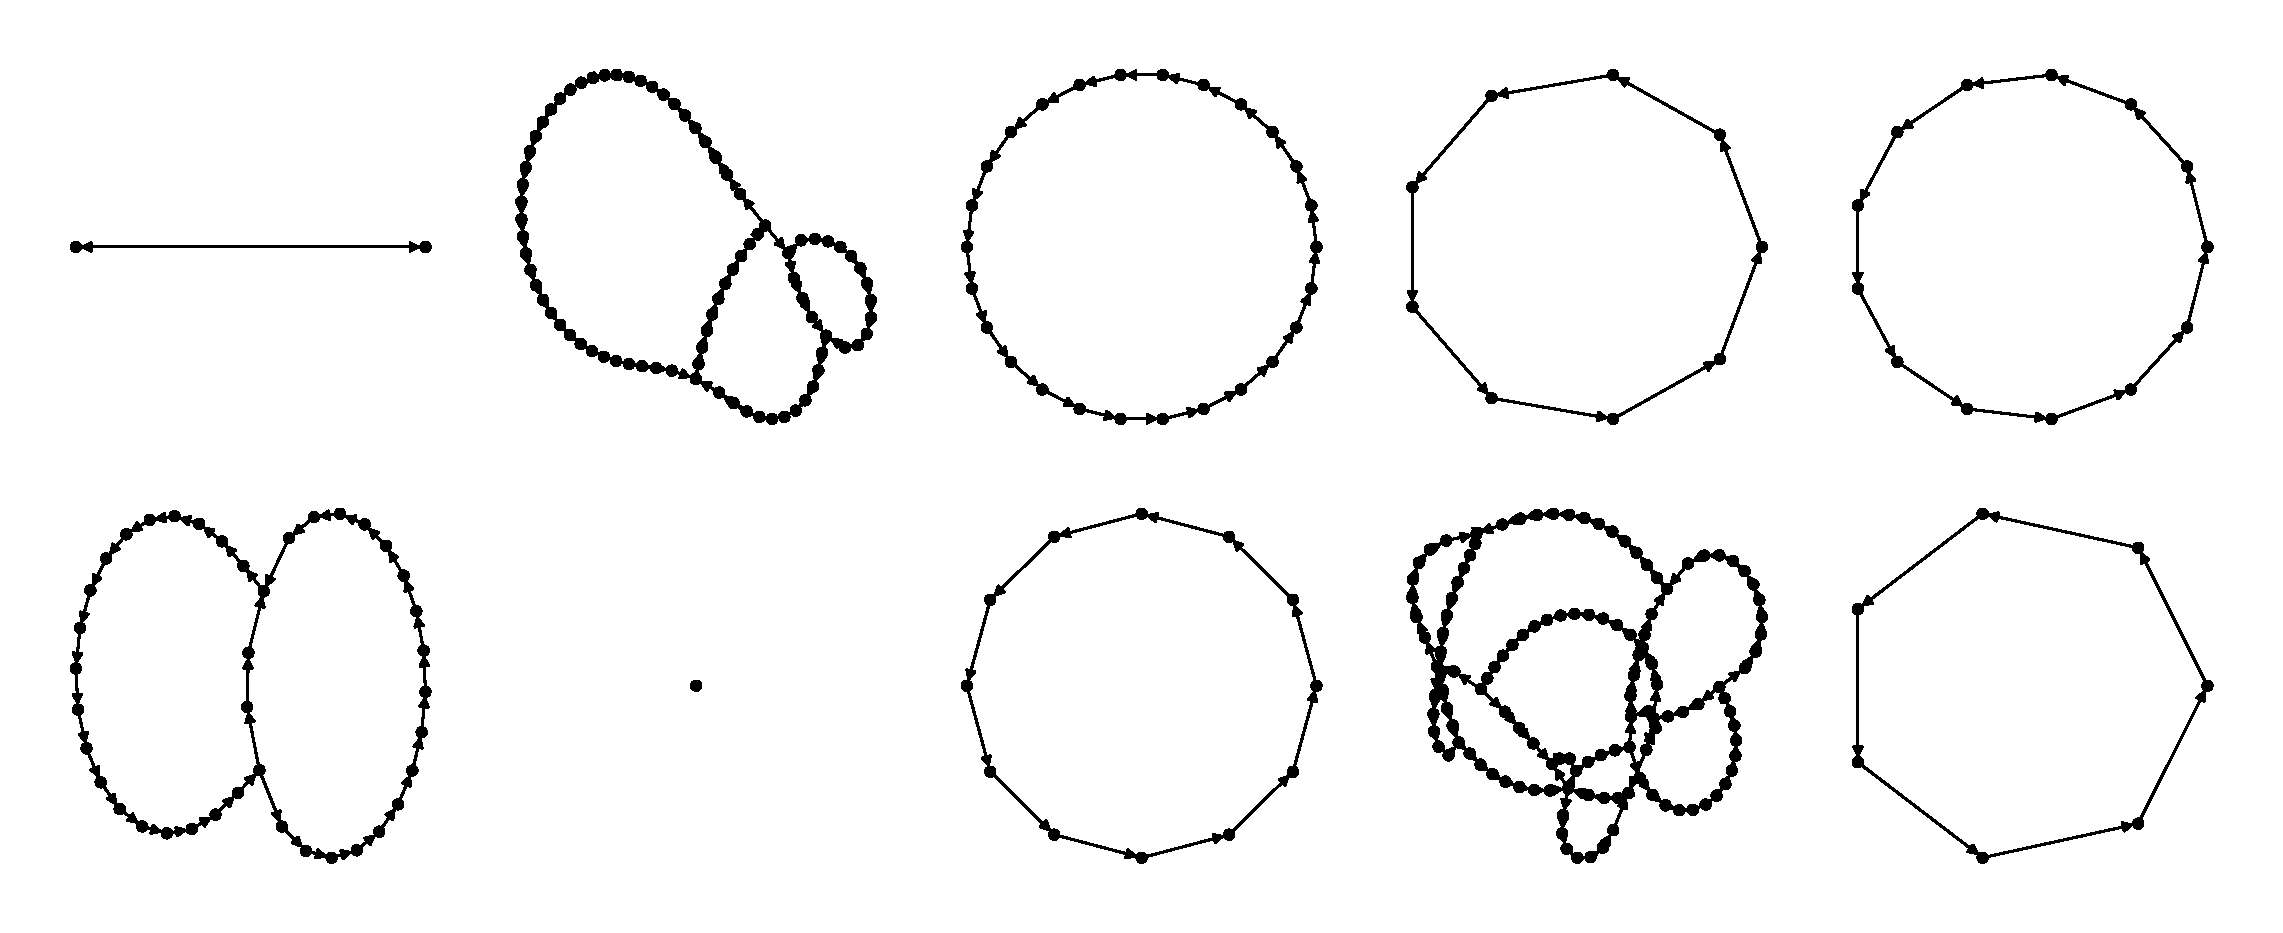
\includegraphics[width=\textwidth]{Content/Pictures/largest_sccs.eps}
    
    \caption{The largest SCC from samples of a directed configuration model with independent $\text{Poisson(1)}$ in- and out-degrees}
    \label{fig:largest-sccs}
\end{figure}

In \cref{fig:largest-sccs} we see the largest SCC from samples of a directed configuration model. As can be seen, while the lengths of paths in the SCC are long, the actual structure of the SCC is often quite simple. Previous work by \citet{goldschmidtScalingLimitCritical2019} shows this is true for the directed Erdős--Renyi model. There it was shown that while the lengths of paths in the SCC will scale like $n^{1/3}$, the actual structure of the SCC will remain finite.

To formalise this idea we will introduce metric directed multigraphs (MDMs). These are simply weighted directed multigraphs, but in our context it is more appropriate to think of the weights as lengths hence the change in naming. Formally a directed multigraph is a tuple $(V, E, r)$ where
\begin{enumerate}
    \item $V$ is a set of vertices,
    \item $E$ is a set of edges, and
    \item $r: E \to V \times V$ is a function mapping edges to their head and tail.
\end{enumerate}
Associated with $r$ are two functions $r_1: E \to V$ and $r_2: E \to V$ such that
\begin{equation*}
    r(e) = (r_1(e), r_2(e))
\end{equation*}
for all $e \in E$. $r_1(e)$ is the tail of the edge $e$ and $r_2(e)$ is the head of the edge $e$. Then a metric directed multigraph (MDM) is a tuple $M = (V, E, r, l)$ where $(V, E, r)$ is a directed multigraph and $l:E \to [0, \infty)$. Let $\zeroloop$ denote the MDM consisting of a single vertex with a self loop of length 0.

An isomorphism between two MDMs $M = (V, E, r, l)$ and $M' = (V', E', r', l)$ is a pair of functions $(i_V, i_E)$ where $i_V: V \to V'$ and $i_E: E \to E'$ are bijections satisfying
\begin{equation*}
    r'(i_E(e)) = (i_V(r_1(e)), i_V(r_2(e)))
\end{equation*}
for all $e \in E$. We say two MDMs are isomorphic if there exists an isomorphism between them. Intuitively this means the MDMS have the same graph structures up to a relabelling of the edges and vertices. Write $\iso(M, M')$ for the set of all isomorphisms between $M$ and $M'$.

We now define a distance $\distmdm$ between two MDMs $M$ and $M'$.  Any isomorphism between $M$ and $M'$ gives a correspondence between the edges of $M$ and the edges of $M'$. We can then take an $\ell_{\infty}$ distance between the lengths of the edges and finally take the isomorphism which minimizes this distance. If $M$ and $M'$ are not isomorphic we can set the distance to be infinite. Formally
\begin{equation*}
    \distmdm(M, M') = \begin{cases}
        \inf_{(i_V, i_E) \in \iso(M, M')} \sup_{e \in E} \abs{l(e) - l(i_E(e))} & \text{if $M$ and $M'$ are isomorphic,} \\
        \infty & \text{otherwise.}
    \end{cases}
\end{equation*}

\begin{figure}[htbp]
    \centering
    \begin{subfigure}[htbp]{0.45\textwidth}
        \centering
        \includegraphics[width=0.95\textwidth]{Content/Pictures/smoothing1.eps}
        \caption{The graph before smoothing $w$}
    \end{subfigure}
    \hfill
    \begin{subfigure}[htbp]{0.45\textwidth}
        \centering
        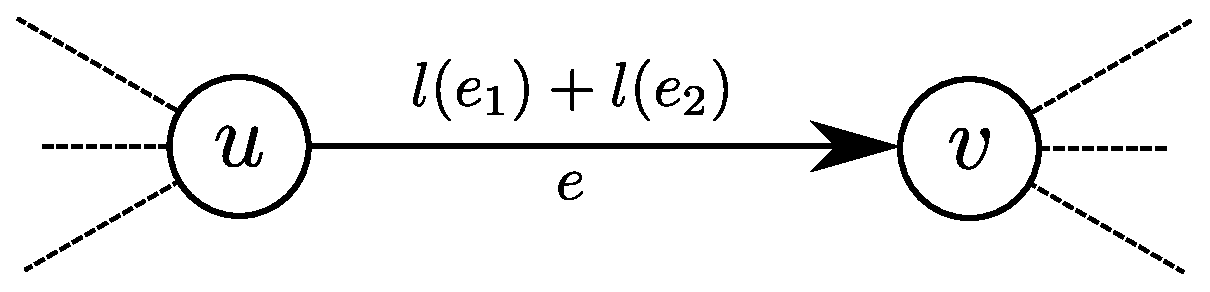
\includegraphics[width=0.95\textwidth]{Content/Pictures/smoothing2.eps}
        \caption{The graph before smoothing $w$}
    \end{subfigure}
    \caption{Smoothing a vertex $w$}
    \label{fig:smoothing}
\end{figure}

\begin{figure}[htbp]
    \centering
    \begin{subfigure}[htbp]{0.45\textwidth}
        \centering
        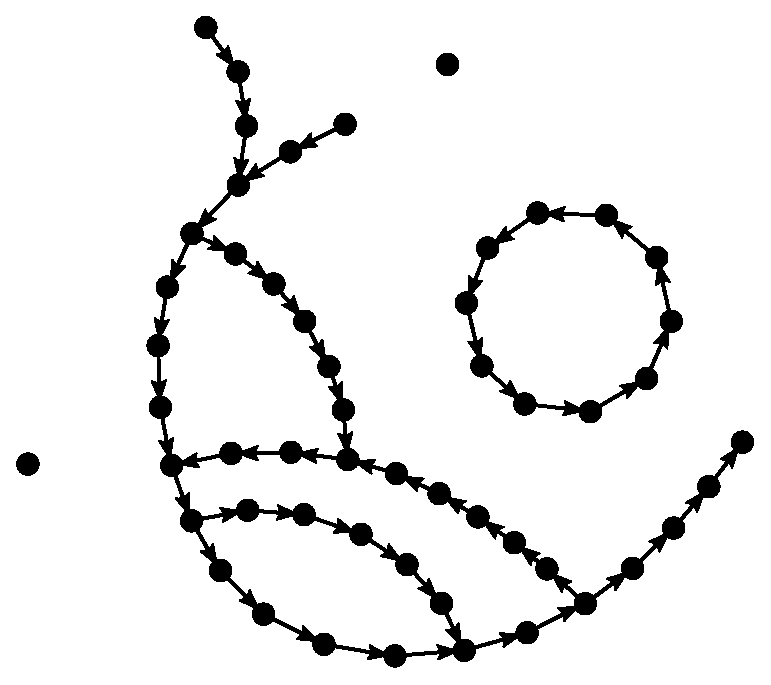
\includegraphics[width=0.90\textwidth]{Content/Pictures/kernel1.eps}
        \caption{$\vec{G}$}
    \end{subfigure}
    \hfill
    \begin{subfigure}[htbp]{0.45\textwidth}
        \centering
        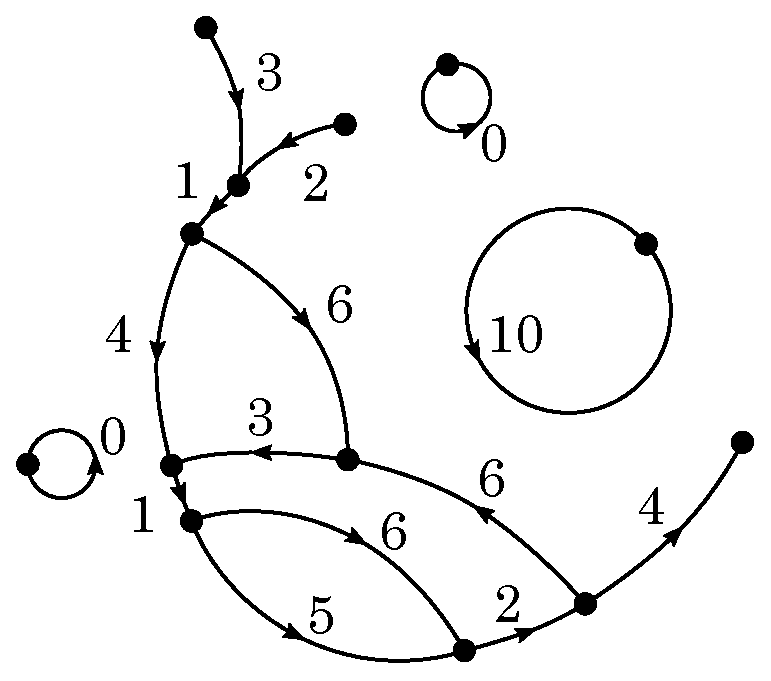
\includegraphics[width=0.90\textwidth]{Content/Pictures/kernel2.eps}
        \caption{$\kernel(\vec{G})$}
    \end{subfigure}
    \caption{An example of a digraph $\vec{G}$ and its kernel $\kernel(\vec{G})$}
    \label{fig:kernel}
\end{figure}

Consider an MDM $M$ and a vertex $w \in M$ with in-degree 1 and out-degree 1 which is not a self-loop. Let $u$ and $v$ be the unique in-neighbour and out-neighbour of $w$ respectively. The MDM obtained by smoothing $w$ is obtained by deleting the edges $e_1$ and $e_2$ such that $r(e_1) = (u, w)$ and $r(e_2) = (w, v)$, then adding an edge $e$ such that $r(e) = (u, v)$ and assigning it length $l(e) = l(e_1) + l(e_2)$. This is illustrated in \cref{fig:smoothing}. Then the kernel of a digraph $\vec{G}$ is obtained by doing the following:
\begin{enumerate}
    \item Assign a length $1$ to each edge.
    \item Iteratively smooth vertices with in-degree 1 and out-degree 1 that are not self-loops until there are none remaining.
    \item Replace all singletons by $\zeroloop$.
\end{enumerate}
Denote the resulting MMD by $\kernel(\vec{G})$. An example is shown in \cref{fig:kernel}.

\subsection{Our results}

Our main result is as follows. Let $C_i(n)$ for $i\geq 1$ be the kernels of the strongly connected components of $\vec{G}_n(\nu)$, listed in decreasing order of size, breaking ties arbitrarily. Complete the list with an infinite repeat of $\zeroloop$. Then, the main theorem is as follows.
\begin{theorem}\label{thm.main}
There exists a sequence $\cC=(\cC_i,i\in \N)$ of random strongly connected MDMs such that, for each $i\geq 1$, $\cC_i$ is either $3$-regular or a loop, and such that 
$$\left(n^{-1/3}C_i(n),i\in \N\right)\overset{d}{\to}\left(\cC_i,i\in \N\right)$$
as $n\to \infty$, with respect to the product $d_{\vec{\cG}}$-topology. The scaling is on lengths in the MDMs.
\end{theorem}
We see here why it is important to consider singletons as loops of length zero. For any fixed $k$, the $k$th largest SCC will not be a singleton with high probability. Therefore no component of our limiting object will be a singleton. Thus we need to pad our SCCs by $\zeroloop$ and consider the kernel of singletons to be $\zeroloop$ so that distance to the limiting object remains finite.

The law of the limit object places our model in the universality class of the directed Erd\H{o}s-Rényi model as studied by \citet{goldschmidtScalingLimitCritical2019}. This is the content of the following Corollary.
\begin{corollary}
Consider $\vec{G}_n(\nu)$, with $\nu$ such that $$\sigma_+=1=\frac{\sigma_{-+}+\nu_-}{\mu}=\frac{\sigma_{-+}+\nu_-}{\mu^2}=1.$$ (Note that this condition is satisfied by $\nu(k^-,k^+)=\nu_1(k^-)\nu_2(k^+)$, with $\nu_i$ the law of a $\operatorname{Poisson}(1)$ random variable.)
Let $(C_i(n), i\geq 1)$ be the strongly connected components of $\vec{G}_n(\nu)$, such that by Theorem \ref{thm.main} there exists $\cC=(\cC_i,i\in \N)$ such that 
$$\left(n^{-1/3}C_i(n),i\in \N\right)\overset{d}{\to}\left(\cC_i,i\in \N\right)$$
as $n\to \infty$, with respect to the product $d_{\vec{\cG}}$-topology. Also consider the directed Erd\H{o}s-R\'enyi model on $n$ vertices, in which any directed edge is present independently with probability $1/n$, which we denote by $\vec{G}(n,1/n)$, and let $(C'_i(n), i\geq 1)$ be the strongly connected components of $\vec{G}_n(\nu)$. Then, also
$$\left(n^{-1/3}C'_i(n),i\in \N\right)\overset{d}{\to}\left(\cC_i,i\in \N\right)$$
as $n\to \infty$, with respect to the product $d_{\vec{\cG}}$-topology. 
\end{corollary}
Moreover, Theorem \ref{thm.main} has the following trivial corollaries, which were previously unknown. 
\begin{corollary}
There exists a random sequence $(\ell_i,i\in \N)\in \R_+^\infty$, such that for $(L^n_i,i\in \N)$ the total lengths in the strongly connected components of $\vec{G}_n(\nu)$ ordered by decreasing length (appended with an infinite repeat of $0$), and for $(S^n_i,i\in\N)$ the number of vertices in the the strongly connected components of $\vec{G}_n(\nu)$ ordered by decreasing size (appended with an infinite repeat of $0$),
$$\left(n^{-1/3}L^n_i,n^{-1/3}S^n_i, i\in \N\right)\overset{d}{\to}\left(\ell_i,\ell_i,i\in \N\right)$$
as $n\to \infty$ in the product topology on $(\R^2)^\infty$. 
\end{corollary}
\begin{corollary}
For $v,w\in \vec{G}_n(\nu)$ such that $v\to w$, let $d(v,w)$ denote the length of the shortest path from $v$ to $w$, and let $$\operatorname{Diam}\left(\vec{G}_n(\nu)\right)=\max\{d(v,w):v\to w\}$$ be the \emph{diameter} of $\vec{G}_n(\nu)$. Then,  $$\operatorname{Diam}\left(\vec{G}_n(\nu)\right)=\Omega(n^{1/3})$$
with high probability.
\end{corollary}


\subsection{Previous work}
The configuration model was introduced by \citet{Bollobas1980} to sample a uniformly random graph with a given degree sequence. For a discussion of the configuration model and proofs of standard results, we refer the reader to \cite[Chapter 7]{hofstadRandomGraphsComplex2017}.

Most results on the configuration model are obtained for models with a deterministic degree sequence. The phase transition for undirected setting was shown in \cite{molloyCriticalPointRandom1995, Molloy1998, Janson2009}. The law of component sizes at criticality and in the critical window were obtained by \citet{Riordan2012} under the assumption that the degrees are bounded. Dhara, van der Hofstad, van Leeuwaarden and Sen showed convergence of the size and surplus edges in the critical window in the finite 3rd moment setting \cite{Dhara2017} and in the heavy-tailed regime \cite{Dhara2020}.  Bhamadi, Dhara, van der Hofstad and Sen obtained metric space convergence in the critical window in \cite{Bhamidi2020}, a result that the authors later improved to a stronger topology in \cite{Bhamidi2020Glmb}. 

Configuration models with a random degree sequence are considered in \cite{josephComponentSizesCritical2014}, \cite{conchon--kerjanStableGraphMetric2020}, and \cite{Donderwinkel2021heightprocess}. \citet{josephComponentSizesCritical2014} showed convergence of the component sizes and surpluses of the large components under rescaling at criticality, both for degree distributions with finite third moments and for the heavy-tailed regime. \citet{conchon--kerjanStableGraphMetric2020} show Gromov-Hausdorff-Prokhorov convergence at criticality in these two regimes. The results in \cite{conchon--kerjanStableGraphMetric2020} in the heavy-tailed regime are extended to the critical window by \citet{Donderwinkel2021heightprocess}. Our techniques are closely related to the techniques introduced in \cite{conchon--kerjanStableGraphMetric2020}. 

Some results have been obtained for other directed graph models. \citet{caoConnectivityGeneralClass2019} consider a class of inhomogeneous directed graphs. Their results include a phase transition for the existence of a giant strongly connected component. This is a generalisation work by \citet{Bloznelis2012}, in which a smaller class of inhomogeneous directed graphs is considered. \citet{Samorodnitsky2016} studied the tails of the degree distribution in the directed preferential attachment model. \citet{goldschmidtScalingLimitCritical2019} studied the directed Erd\H{o}s-R\'enyi model, and were the first to obtain metric space convergence of the strongly connected components of a directed graph. Our methods build on their techniques.

The directed configuration model was first considered by \citet{cooperSizeLargestStrongly2004}. They consider a deterministic degree sequence under a number of conditions, and show that for $\theta$ the expected in-degree of a uniformly chosen vertex, and $\rho$ the expected product of in-degree and out-degree of a uniformly chosen vertex, a phase transition for the strongly connected components occurs at $d=\theta/\rho=1$. They show that for $d<1$, with high probability, all strongly connected components contain $O(\Delta\log(n))$ vertices, for $\Delta$ the maximal degree. On the other hand, for $d>1$, there is a unique strongly connected components that contains a positive proportion of the vertices and also $O(n)$ edges. Their conditions are restrictive, and include finite second moments of both the in- and out-degree of a uniformly chosen vertex, and a bound of size $n^{1/12}/\log(n)$ on the largest degree. Their proofs are based on an algorithm to explore the directed graph. The condition on the largest degree was later relaxed to $O(n^{1/4})$ by \citet{Graf2016}.\myworries{check this is the phase transition}

Recently, Cai and Perarnau have obtained a number of results on the directed configuration model with deterministic degrees. In \cite{caiDiameterDirectedConfiguration2020}, they show, under first and second moment conditions of the degree of a uniformly picked vertex, for $d\neq 1$ (i.e. not at criticality), that the diameter of the model on $n$ vertices, rescaled by $\log(n)$ converges to a constant that they identify. Then, in \cite{caiGiantComponentDirected2020}, they show a law of large numbers for the number of vertices and edges in the largest strongly connected component, under slightly stronger moment conditions, and again not at the critical point. In \cite{cai2021rw}, they study the behaviour of a random walk on a directed configuration model.
 
The emergence of a giant weakly connected component for the directed configuration model with a deterministic degree sequence is discussed in the physics literature by \citet{Kryven2016}. He also studies the distribution of the in- and out-components in \cite{Kryven2017}.

The directed configuration model with random in- and out-degrees is also considered by \citet{Chen2012}, although, importantly, they do not allow for the in- and out-degree of a vertex to be dependent. The authors consider a model in which the in- and out-degrees are two independent sequences of i.i.d.\ random variables drawn from two probability distributions. They propose an algorithm to sample degree sequences that correspond to a simple graph and show the limiting distribution of the degrees generated by this algorithm. 


\subsection{Proof outline}

The techniques we will use to investigate the graph model are a combination of the techniques introduced by Conchon-Kerjan and Goldschmidt in \cite{conchon--kerjanStableGraphMetric2020} and the strategy of Goldschmidt and Stephenson in \cite{goldschmidtScalingLimitCritical2019}. The former work discusses the scaling limit of an undirected uniform graph with i.i.d.\ degrees at criticality, and the latter discusses the scaling limit of the strongly connected components of a directed Erd\H{o}s-Renyi graph at criticality.

To investigate the structure of the strongly connected components of a uniform graph with degree sequence $(\mathbf{D}_1,\dots,\mathbf{D}_n)$, conditional on $\sum_{i=1}^n D^-_i=\sum_{i=1}^n D^+_i$, we will use a version of the configuration model for digraphs that was introduced by \citet{cooperSizeLargestStrongly2004}.

Consider a degree sequence $\vd_1, \ldots, \vd_n$ where $\vd_i = (d_i^-, d_i^+) \in \N \times \N$. We assume 
\begin{equation*}
    \textstyle\sum_{i=1}^n d_i^- = \sum_{i=1}^n d_i^+. 
\end{equation*}
To sample the \emph{directed configuration model} with degree sequence $\vd_1, \ldots, \vd_n$ let $v_1, \ldots, v_n$ be vertices such that $v_i$ has $d_i^-$ in-half-edges and $d_i^+$ out-half-edges. We then pair the in-half-edges and out-half-edges uniformly. This results in a random directed multigraph. The directed configuration model is obtained by This is illustrated in Figure \ref{fig.configuration model}. 

If we then condition on the multigraph being simple, we would get a uniform random digraph on $[n]$ conditioned to have the given degree sequence. This is shown by \citet[P. 10--11]{cooperSizeLargestStrongly2004}. 

To explore the structure of a directed multigraph, we describe an edge-based depth first search procedure (eDFS) in \cref{alg:edfs}. This takes as input a directed multigraph and uses a stack of edges. When the stack is empty, we are at the start of a new out-component and thus pick a new vertex $w$ with probability proportional to its in-degree (this choice simplifies \myworries{insert lemma}). Otherwise we remove the last edge $(v, w)$ off the stack. In both cases, if $w$ has not yet been explored, we add the out-edges from this vertex to the end of the stack of edges (this choice is what makes the exploration depth first).

\myworries{define surplus edges and ordering of vertices}

At each step we also maintain $S^-(k)$ and $S^+(k)$. $S^-(k)$ keeps track of the number of in-edges which we have seen but have not explored the tail of yet at step $k$. $S^+(k)$ is akin to a Lukasiewiescz path. At any given step it is equal to the size of the stack of edges after subtracting the number of fully explored out-components.

We also construct a directed forest for which $S^-(k)$ will be a true Lukasiescz path. At each step of the process we will be examining a vertex $w$. If $w$ has not been explored yet then either we are at the start of a new out-component, in which case we add $w$ to the out-forest, or we are exploring an edge $(v, w)$ where $v$ has already been explored and added to the out-forest, in which case we add $w$ and the edge $(v, w)$ to the out-forest. If $w$ has already been explored we cannot add $(v, w)$ to the out-forest without creating loops. Instead add a dummy vertex to the out-forest and an edge from $v$ to the dummy vertex. We call such dummy vertices purple leafs. This is illustrated in Figure \ref{fig.configuration modeloutforest}. We refer to the out-forest corresponding to the exploration up to time $k$ as $\hat{F}_n(k)$.

\def \exploredvertices {\mathcal V}
\def \explorededges {\mathcal E}
\def \forest {\mathcal F}
\def \edgestack {\mathcal O}
\begin{algorithm}[htbp]
    \SetAlgoLined
    \KwData{A directed multigraph}
    $\exploredvertices \leftarrow$ an empty ordered list of vertices\;
    $\edgestack \leftarrow$ an empty ordered list of edges\;

    $k \leftarrow 0$ \;
    $S^- \leftarrow 0$ \;
    $S^+ \leftarrow 0$ \;
    $\forest \leftarrow$ an empty directed graph\;
    \While(){there exists unexplored vertices of positive in-degree}{
        \eIf(){$\edgestack$ is empty}{
            $w \leftarrow$ a random vertex not in $\exploredvertices$ chosen with prob.\ proportional to $d^-(w)$ \;
        }(){
            $e \leftarrow$ last edge in $\edgestack$ \;
            remove $e$ from $\edgestack$ \;
            $v \leftarrow$ tail of $e$\;
            $w \leftarrow$ head of $e$ \;
            $S^- \leftarrow S^- - 1$ \;
        }
        \eIf(){$w \not \in \exploredvertices$}{
            append $w$ to $\exploredvertices$ \; 
            add the vertex $w$ to $forest$ \;
            \If(){$\edgestack$ is non-empty}{
                add the edge $(v, w)$ to $\forest$\;
            }
            append all out-edges of $w$ to the end of $\edgestack$ in a uniform random order \;
            $S^- \leftarrow S^- + d^-(w)$ \;
            $S^+ \leftarrow S^+ + d^+(w) - 1$ \;
        }{
            add a purple leaf to $\forest$ and and edge from $v$ to the leaf \;
        }
        $k \leftarrow k + 1$ \;
        $S^-_k \leftarrow S^-$ \;
        $S^+_k \leftarrow S^+$ \;
        $\forest_k \leftarrow \forest$ \;
    }
    \caption{The eDFS procedure \label{alg:edfs}}
\end{algorithm}

\begin{figure}
    \centering
    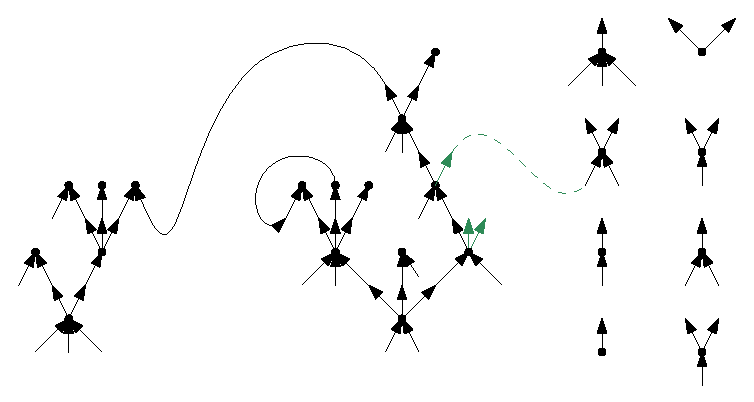
\includegraphics[scale=0.6]{Content/Pictures/configuration_model.eps}
    \caption{The green arrows represent unpaired out-half-edges of vertices that have been visited. One by one, in depth first order, these are paired to a uniform unpaired in-half-edge.}
    \label{fig.configuration model}
\end{figure}

An important motivation for studying the out-forest is the fact that the vertex set of any strongly connected component is contained in one of the components of the out-forest. This is a straightforward property that is further discussed in Lemma \ref{lemma.whatispartofscc}. We have defined the out-forest in such a way that every time step in the exploration corresponds to one vertex in the out-forest. 

A key fact is that the order in which the vertices are discovered does not depend on the position of the purple vertices. Similarly, the position of the purple vertices does not depend on the position of the heads of the surplus edges. Furthermore, we define a necessary condition for a surplus edge to be part of a strongly connected component (see Definition \ref{def.candidate} and Corollary \ref{cor.edgesinSCCs}), and we call these surplus edges \emph{candidates}. The candidates are defined in such a way that whether a purple vertex is a candidate does not depend on the position of the heads of the surplus edges. This allows us to define the following sampling procedure.
\begin{enumerate}
    \item We sample the order of discovery of the vertices in the exploration.
    \item We sample at which time steps a surplus edge is added instead of an edge to an undiscovered vertex, which allows us to define the out-forest $(\hat{F}_n(k),k\geq 1)$. 
    \item We visit the purple vertices in $(\hat{F}_n(k),k\geq 1)$ in depth-first order, and for each vertex we sample whether it corresponds to a candidate.
    \item We visit the tails of the candidates in depth-first order, and for each of them, sample where the head of the corresponding surplus edge is.
\end{enumerate}

\begin{figure}
    \centering
    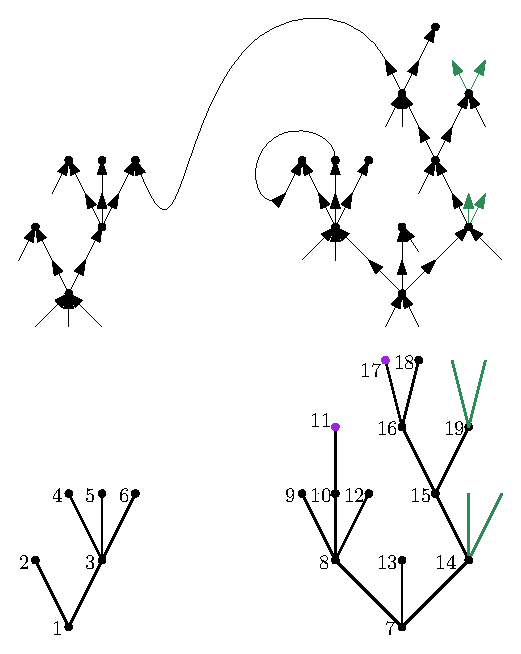
\includegraphics[scale=0.8]{Content/Pictures/configuration_model_out_forest.eps}
    \caption{The out-forest is defined based on the exploration of the digraph. For each surplus edge, we add an extra leaf, which we colour purple. The labels of the vertices correspond to the time step in the exploration at which the vertex is added. The green edges lead to vertices of which the degree and colour have not yet been sampled.}
    \label{fig.configuration modeloutforest}
\end{figure}
Then, our approach is as follows.
\begin{enumerate}
    \item We find the limit under rescaling of the \L ukasiewicz path and height process of $\hat{F}_n(m_n)$ for $m_n=O(n^{2/3})$ conditional on $\sum_{i=1}^n D^-_i=\sum_{i=1}^n D^+_i$ and simplicity of the digraph. (For a definition of the \L ukasiewicz path and height forest, see \cite{AST_2002__281__R1_0}, Chapter 0.)
    \item We show that the positions of the tails of the candidates converge.
    \item We show that the positions of the heads of the candidates converge.
    \item We identify the tails and heads of the candidates, and recover the strongly connected components from the resulting digraph with a cutting procedure. We use a result in \cite{goldschmidtScalingLimitCritical2019} that implies that the cutting procedure converges.
    \item We show that for any $\delta>0$, with high probability, all strongly connected components with length larger than $\delta n^{1/3}$ are contained in the exploration up to time $O(n^{2/3})$. Therefore, we can choose $m_n$ such that, with high probability, we do not miss any large strongly connected components by not considering the exploration beyond time $m_n$. This finishes the proof of the convergence in the product topology.
\end{enumerate}

\subsection{Open problems}
Our work contains the first results on the directed configuration model at criticality, and is the second metric space convergence result for a directed graph model (after the directed Erd\H{o}s-Rényi graph was studied in \cite{goldschmidtScalingLimitCritical2019}), so naturally, there are many interesting unresolved questions.
\begin{enumerate}
    \item The law of our limit object is defined by three parameters that are functions of the (mixed) moments of the degree distribution. Does a different choice of parameters always give a different limit distribution? If so, are the laws absolutely continuous to one another?
    \item Our methods show that the diameter of the configuration model at criticality is  $\Omega(n^{1/3})$, which is in contrast with the off-critical cases (for deterministic degrees), in which the diameter is $O(\log(n))$ \cite{caiDiameterDirectedConfiguration2020}. We believe that the diameter is in fact exactly $O(n^{1/3})$. Goldschmidt and Maazoun are working on this question for the directed Erd\H{o}s-Rényi graph at criticality. 
    \item In \cite{goldschmidtScalingLimitCritical2019}, the authors show convergence of the sequence of SCCs in the $\ell_1$-sense, which is stronger than the product topology as considered by us. This for example implies that for the directed Erd\H{o}s-Rényi graph, the total length in the SCCs converges in distribution to some finite number. Also for undirected configuration models, there are no results that show metric space convergence in a topology on the sequence of components that is stronger than the product topology \cite{Bhamidi2020}\cite{conchon--kerjanStableGraphMetric2020}\cite{Bhamidi2020Glmb}.
     \item We conjecture that, just like the directed Erd\H{o}s-Rényi graph \cite{goldschmidtScalingLimitCritical2019}, the directed configuration model gives rise to a critical window, that in some sense interpolates between subcritical and supercritical models. It would be interesting to adapt our methods to the critical window.
     \item We plan to extend our understanding of the strongly connected components by studying the directed graphs that they are embedded in. A first step would be to study all vertices that can be reached from the non-trivial strongly components. This would illuminate connections between the strongly connected components and expose the fractal structure of the directed graph, which is not observed when only studying the strongly connected components themselves.
    \item Another natural next step is to study the model under weaker moment conditions. The first condition to eliminate is $\E\left[(D^-)^i(D^+)^j\right]$ for $\{i,j\}=\{1,3\}$, which would in some sense makes the identifications less uniform on the ancestral lines. We have reason to believe that this would place the model in  a different universality class, but further research is needed to confirm this. Also the heavy-tailed case is not well-understood, but given our results, it is natural to expect the limit object to be embedded in a tilted stable tree as defined in \cite{conchon--kerjanStableGraphMetric2020}. Moreover, one could define hybrid models by letting the tail-behaviour of the in- and out-degrees be different. 
    \item We conjecture that the inhomogeneous directed random graph model under suitable conditions is part of the same universality class as the directed Erd\H{o}s-Rényi graph \cite{goldschmidtScalingLimitCritical2019} and $\vec{G}_n(\nu)$. We believe that our methods and the methods of \cite{goldschmidtScalingLimitCritical2019} can be adapted to obtain a metric space scaling limit for the inhomogeneous directed random graph model. 

\end{enumerate}


\section{Sampling the MDM in the discrete and the continuum}
If we forget about the directions of the edges in $\vec{G}_n(\nu)$, the resulting undirected graph is supercritical, and, with high probability, the graph contains a unique giant component with surplus going to infinity as $n\to \infty$ (see e.g. \cite{molloyCriticalPointRandom1995,Molloy1998,Janson2009} for a discussion of the phase transition in the undirected configuration model). This suggests that if we do not dismiss a large amount of edges, we will not be able to study the digraph in enough detail to find a metric space scaling limit of the SCCs. Therefore, we will not try to sample the entire digraph, but focus on the information that we need to find the SCCs. We start by studying the discrete digraph model, with the goal of identifying which edges can be part of an SCC, and how to sample them. In Subsection \ref{subsubsec.defcandidates}, we establish necessary conditions for an edge to be part of an SCC. These conditions imply that we only need to study the out-forest, and the surplus edges corresponding to a small subset of the dummy leaves. We call these dummy leaves \emph{candidates}. In Subsections \ref{subsubsec.samplingoutforest} and \ref{subsubsec.samplecandidates} we study the law of the out-forest and the candidates respectively, and we define a procedure to sample them both. This yields a sequence of directed multigraphs with edge lengths in which the SCCs are embedded.  
In Subsection \ref{subsec.limitobject}, we define the continuous counterpart of the sampling procedure. The resulting object will be the limit under rescaling of the sequence of directed multigraphs with edge lengths in which the SCCs are embedded that was constructed in Subsections \ref{subsubsec.samplingoutforest} and \ref{subsubsec.samplecandidates}. 
\subsection{The discrete case}\label{subsec.discrete}
We will discuss the different type of edges that we can encounter in the exploration. Recall from Subsection \ref{sec:proofoutline} that by slight abuse of terminology, we call the dummy leaf that corresponds to a surplus edge its tail.

\subsubsection{Necessary conditions for an edge to be part of an SCC}\label{subsubsec.defcandidates}
Amongst the surplus edges, \emph{ancestral surplus edges}, which are surplus edges that point from a vertex to one of its ancestors, play a special role. All other surplus edges are called \emph{non-ancestral}. This is illustrated in Figure \ref{subfigure.typesofsurplusedges}. In Figure \ref{subfigure.sccinexample} we show how surplus edges affect the structure of the SCCs. This is the content of the next lemma.
\begin{lemma}\label{lemma.whatispartofscc}
The following facts hold for SCCs. 
\begin{enumerate}
\item \label{item.factsonsccs1}The vertices of an SCC are contained in precisely one of the components of {$(\hat{F}_n(k),k\geq 1)$}. 
\item \label{item.factsonsccs2} Ancestral surplus edges are always part of an SCC.
\item \label{item.factsonsccs4} A non-ancestral surplus edge is part of an SCC only if its head is an ancestor of the tail of a surplus edge that is part of an SCC.
\item \label{item.factsonsccs4andabit} An edge in $(\hat{F}_n(k),k\geq 1)$ is part of an SCC only if its head is an ancestor of the tail of a surplus edge that is part of an SCC.
\item \label{item.factsonsccs5} For any non-trivial SCC, the first surplus edge of the SCC that is explored is an ancestral surplus edge, and a component of  $(\hat{F}_n(k),k\geq 1)$ contains an SCC if and only if it contains an ancestral surplus edge.
\end{enumerate}
\end{lemma}
\begin{proof}
We start with \ref{item.factsonsccs1}. Let $v$ and $w$ be two vertices in the same SCC. Without loss of generality, $v$ is explored first in depth-first order in the out-direction. Since $v$ and $w$ are part of the same SCC, we know that there is a path from $v$ to $w$ in the out-direction. This implies that $w$ will be part of the out-subtree consisting of the descendants of $v$. This implies that they are part of the same component of $(\hat{F}_n(k),k\geq 1)$.

To prove \ref{item.factsonsccs2}, suppose there is an ancestral surplus edge from $v$ to $w$. This implies that $w$ is an ancestor of $v$ in an out-component, which implies that there is a path from $w$ to $v$ as well. It follows that $w$ and $v$ are in the same SCC and that the ancestral surplus edge from $v$ to $w$ is in this SCC as well. 

To prove \ref{item.factsonsccs4} and \ref{item.factsonsccs4andabit}, suppose there is a non-ancestral surplus edge from $v$ to $w$ that is part of an SCC, or that $(v,w)$ is an edge of $(\hat{F}_n(k),k\geq 1)$ that is part of an SCC. Then, there is some directed path $(x_0,\dots, x_m)$ with $x_0=w$ and $x_m=v$. Let $k$ be minimal such that $x_k$ is not a descendant of $w$ (such a $k$ exists, because by assumption, $v$ is not a descendant of $w$). Then, $(x_{k-1},x_k)$ is a surplus edge that is in the same SCC as $v$ and $w$, and $x_{k-1}$ is a descendant of $v$. 


Finally, \ref{item.factsonsccs2} and \ref{item.factsonsccs4} imply \ref{item.factsonsccs5}. 
\end{proof}

Lemma \ref{lemma.whatispartofscc} motivates the following definition.
\begin{definition}\label{def.candidate}
A surplus edge is a \emph{candidate} if either
\begin{itemize}
    \item It is an ancestral surplus edge, or
    \item One of the descendants of its head is the tail of a candidate.
\end{itemize}
\end{definition}
The following corollary is at the core of our strategy to study the SCCs.
\begin{corollary}\label{cor.edgesinSCCs}
Any edge that is part of an SCC is either a surplus edge corresponding to a candidate, or is contained in the subforest of $(\hat{F}_n(k),k\geq 1)$ that is spanned by the tails of candidates and the roots of the out-components.
\end{corollary}
\begin{proof}
This follows from Definition \ref{def.candidate} and parts \ref{item.factsonsccs1}, \ref{cond.excursions2}, \ref{item.factsonsccs4} and \ref{item.factsonsccs5} of Lemma \ref{lemma.whatispartofscc}.
\end{proof}
\begin{figure}
\centering
\begin{subfigure}{0.7\textwidth}
 \centering
    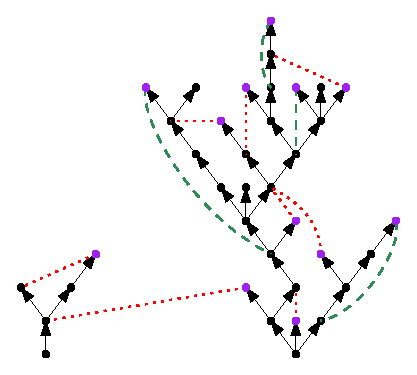
\includegraphics[width=0.7\linewidth]{Content/Pictures/types_of_surplus_edges.eps}
    \caption{This figure illustrates an example of a depth-first exploration of two out-components with the different type of surplus edges highlighted. The ancestral surplus edges (green dashed) point from a vertex $v$ to one of its ancestors. They are always part of an SCC. The other surplus edges are depicted as red dotted lines.}
    \label{subfigure.typesofsurplusedges} 
\end{subfigure}\\
\begin{subfigure}{0.7\textwidth}
  \centering
  \includegraphics[width=0.7\linewidth]{Content/Pictures/sccs_in_example.eps}
  \caption{The non-trivial SCCs embedded in the components of the out-forest are depicted in orange, blue and green. The trivial SCCs are black. The grey edges are not part of an SCC, and the grey vertices correspond to dummy leaves that are not part of an SCC.}
    \label{subfigure.sccinexample}
\end{subfigure}
\caption{We illustrate the different types of surplus edges and how they affect the structure of the SCCs.}
\end{figure}

Corollary \ref{cor.edgesinSCCs} implies that to sample the SCCs, we do not need to sample the heads corresponding to all dummy leaves. Instead, for every dummy leaf, we only need to know whether it is a candidate, and if so, where its head is. 
\subsubsection{Sampling the out-forest}\label{subsubsec.samplingoutforest}
This subsection discusses how to obtain the out-forest conditional on the order in which the vertices are discovered. We will study the law of the degrees in order of discovery in Subsection \ref{subsec.measurechange}. The out-forest is obtained in the following way. Let
\begin{equation*}
    \cI_n = \{i \in [n]: D_i^- > 0\}
    \quad \text{and} \quad
    R_n = \abs{\cI_n},
\end{equation*}
so that $R_n$ is the number of vertices with positive in-degree. Suppose the degrees in order of discovery (as given by $\exploredvertices$ in the eDFS algorithm) are given by $(\mathbf{\hat{D}}_{n,1},\dots,\mathbf{\hat{D}}_{n, R_n})$. Up to time-step $k$, suppose we have added the vertices corresponding to the first $m\leq k$ elements of  $(\mathbf{\hat{D}}_{n,1},\dots,\mathbf{\hat{D}}_{n, R_n})$ to the forest. We call these vertices \emph{discovered}. Then, at time $k+1$,
\begin{enumerate}
    \item If we have finished a component of the out-forest, let the next out-component have a root with out-degree $\hat{D}_{n,m+1}^+$. 
    \item Otherwise,
    \begin{enumerate}\item With probability proportional to the total in-degree of the undiscovered vertices, i.e. $\sum_{i={m+1}}^{R_n} \hat{D}_{n,i}^-$, let the next vertex in depth-first order be a black vertex with out-degree $\hat{D}_{n,m+1}^+$. 
    \item With probability proportional to the number of unpaired in-half-edges of the $m$ discovered vertices, let the next vertex in depth-first order be a dummy leaf, and reduce the total number of unpaired in-edges of the $M$ discovered vertices by $1$.
\end{enumerate}
\end{enumerate}
We make this rigorous in the following lemma.
\begin{lemma}\label{lemma.sampleoutforest}
Suppose the sequence of degrees in order of discovery $(\mathbf{\hat{D}}_{n,1},\dots,\mathbf{\hat{D}}_{n, R_n})$ is given. Suppose, for $1\leq l\leq k$, that up to time $l$, $\hat{P}_n(l)$ surplus edges have been sampled. Then, $$\left(\hat{S}^+_n(l),1\leq l\leq k \right):=\left(\sum_{i=1}^{l-\hat{P}_n(l)}\hat{D}^+_{n,i}-l,1\leq l\leq k\right)$$ is the \L ukasiewicz path of the out-forest up to time $k$. Moreover, for $$\left(\hat{I}^+_n(l),1\leq l\leq k\right):=\left(\min\left\{\hat{S}^+_n(m):1\leq m \leq l\right\},1\leq l \leq k \right),$$
define 
$$\left(\hat{S}^-_n(l),1\leq l \leq k\right):=\left(\sum_{i=1}^{l-\hat{P}_n(l)}\hat{D}^-_{n,i}-l-\hat{I}^+_n(l)+1,1\leq l\leq k\right),$$
so that $\hat{S}^-_n(k)$ is equal to the number of unpaired in-half-edges of discovered vertices at time $k$. Then, the probability that we sample a surplus edge at the $(k+1)^{th}$ time-step is given by
$$\frac{\hat{S}^-_n(k+1)}{\sum_{i=1}^n D^-_i-k-\hat{I}^+_n(k)+1}\one_{\left\{\hat{I}^+_n(k)=\hat{I}^+_n(k-1)\right\}}.$$
Therefore, we do not need to know the position of the heads of the surplus edges in order to sample the out-forest.
\end{lemma}
\begin{proof}
Note that if up to time $k$, $\hat{P}_n(k)$ surplus edges have been sampled and this implies that $k-\hat{P}_n(k)$ true vertices have been discovered. Thus, up to time $k$, the out-forest contains $\hat{P}_n(k)$ dummy leaves, and true vertices with degrees $(\hat{D}^+_{n,1},\dots,\hat{D}^+_{n,k-\hat{P}_n(k)})$, so by definition of the \L ukasiewicz path, its value is indeed equal to $\hat{S}^+_n(k)$ at time $k$. Moreover, up to time $k$, the total in-degree of the discovered true vertices is equal to $\sum_{i=1}^{k-\hat{P}_n(k)}\hat{D}^-_{n,i}$. At every time step, we pair one in-half-edge of a discovered vertex, unless we start a new component. The value $-\hat{I}^+_n(k)$ corresponds to the number of out-components that are fully explored up to time $k$, so the total number of unpaired in-half-edges of discovered vertices at time $k$ is equal to $\hat{S}^-_n(k)$. By the same reasoning, the total number of unpaired in-half-edges is equal to $\sum_{i=1}^n D^-_i-k-\hat{I}^+_n(k)+1$. The probability of sampling a surplus edge at step $(k+1)$ follows. We note that this probability does not depend on the positions of the heads of the earlier surplus edges, but only on their number, which implies that we can sample the out-forest without sampling the positions of the heads.
\end{proof}
\subsubsection{Sampling the candidates}\label{subsubsec.samplecandidates}
We will now study the law of the candidates conditional on $(\hat{F}_n(k),k\geq 1)$. As before, for each $k$, let $\hat{P}_n(k)$ denote the number of dummy leaves amongst the first $k$ vertices in the out-forest, and let $\hat{S}^-(k)$ denote the number of unpaired in-half-edges of discovered vertices at time $k$. We will first identify the tails of the candidates amongst the dummy leaves, and then we will sample the positions of their heads. \\
If the vertex visited at time $k$ is a dummy leaf, the head of the corresponding surplus edge is a uniform pick from the $\hat{S}^-(k)$ unpaired in-half-edges of discovered vertices at time $k$. Therefore, the probability that a dummy leaf visited at time $k$ corresponds to an ancestral surplus edge is given by the number of unpaired in-edges on its path to the root divided by $\hat{S}^-(k)$. This implies that to understand the law of the position of ancestral surplus edges, we need to understand where the unpaired in-edges are. \\
We will study this by modifying the edge lengths in the tree: for a vertex $v$ with in-degree $m$, the edges connecting it to its children will all have length $m-1$ (unless $v$ is the root of an out-component, in which case the edges connecting to its children will be assigned length $m$). The height of vertex $w$ in this forest with modified edge lengths corresponds to the number of in-half-edges that can be used to form an ancestral surplus edge with tail $w$. We add lengths to all edges in $(\hat{F}_n(k),k\geq 1)$ and call the resulting forest with edge lengths $(\hat{F}^\ell_n(k),k\geq 1)$. Denote the height process of $(\hat{F}^\ell_n(k),k\geq 1)$ by $(\hat{H}_n^\ell(k),k\geq 1)$. \\
Recall that the first candidate in any component of $(\hat{F}_n(k),k\geq 1)$ is an ancestral surplus edge. The following lemma illustrates the importance of $\hat{H}^\ell$ in finding the first ancestral surplus edges in the out-components.

\begin{lemma}\label{lemma.probancestral}
Consider the exploration of $(\hat{F}_n(l),l\geq 1)$ at time $k$. If no ancestral surplus edge has been sampled in the current component, then the probability that $k$ is the tail of an ancestral surplus edge is given by 
$$\frac{\hat{H}^\ell(k)}{\hat{S}_n^-(k)}\one_{\{\hat{P}_n(k)-\hat{P}_n(k-1)=1\}}.$$
This event is conditionally independent of the positions of the heads of the surplus edges that were found before time $k$, given that none of them were ancestral in the current component.
% If $k$ is the tail of an ancestral surplus edge, then the position of the end point $Y$ has the following law. Let $U$ be uniform on $[0,\hat{H}^\ell(k)]$. Then, let $Y_k$ be the height of youngest ancestor $l$ of $k$ such that $H^{\ell}(l)<U$. 
\end{lemma}
\begin{proof}
We claim that if no ancestral surplus edge has been sampled in the current component, none of the ancestors of $k$ are the head of a surplus edge. Indeed, for $x$ an ancestor of $k$, all vertices that are visited since the discovery of $x$ up to time $k$ are descendants of $x$, because $(\hat{F}_n(k),k\geq 1)$ is explored in a depth-first manner. Therefore, any surplus edge with head $x$ sampled up to time $k$ is ancestral. This implies that for $d^-$ the in-degree of $x$, the number of unpaired in-half-edges of $x$ at time $k$ is equal to $d^--1$ (unless $x$ is the root of the out-component, in which case it has $d^-$ unpaired in-half-edges).

Therefore, the number of unpaired in-half-edges corresponding to ancestors of $k$ is equal to $H^\ell(k)$. Moreover, note that, by definition of the dummy leaves, $k$ is the tail of a surplus edge if and only if $k$ is purple, i.e. if and only if $\hat{P}_n(k)-\hat{P}_n(k-1)=1$. In that case, the probability that it connects to given unpaired in-half-edge of a visited vertex is equal to $1/\hat{S}_n^-(k)$. The stated probability follows. The independence of the positions of the heads of earlier surplus edges is immediate.
\end{proof}

We now illustrate how to find the other candidates in a component of $(\hat{F}_n(k),k\geq 1)$. 
\begin{lemma}\label{lemma.samplecandidates}
Let $T^n_{l_n}$ be a component of $(\hat{F}_n(k),k\geq 1)$ with root $l_n+1$ and component size $\sigma_n$. Suppose the first ancestral surplus edge with vertices in $T^n_{l_n}$ corresponds to dummy leaf $V^n_1\in [l_n+2,l_n+\sigma_n]$. Let $V^n_1<k\leq l_n+\sigma_n$, and suppose the candidates found up to time $k$ are given by $V^n_1,\dots,V^n_m$. Let $T^{n,\mathrm{mk}}_k$ be the subtree of $T^n_{l_n}$ spanned by $\{l_n+1,V^n_1,\dots,V^n_m,k\}$, and let $\ell(T^{n,\mathrm{mk}}_k)$ be its total length with edge lengths as defined by $(\hat{H}^\ell(i),i\in [l_n+1,l_n+\sigma_n])$. Then, the probability that $k$ is a candidate is given by 
$$\frac{\ell\left(T^{n,\mathrm{mk}}_k\right)-m}{\hat{S}^-(k)}\one_{\{\hat{P}_n(k)-\hat{P}_n(k-1)=1\}}.$$
\end{lemma}
\begin{proof}
Note that if $k$ is purple, it gets paired to a uniform pick from the $\hat{S}^-(k)$ unpaired in-half-edges of discovered vertices. By Definition \ref{def.candidate}, in that case, $k$ is a candidate if and only if its head is in $T^{n,\mathrm{mk}}_k$. Observe that $\ell\left(T^{n,\mathrm{mk}}_k\right)$ is equal to the number of in-half-edges of $T_{k}$ that can be used to form surplus edges. By the definition of a candidate, exactly $m$ of those have been paired: one for each element in $\{V^n_1,\dots,V^n_m\}$. This implies that $\ell\left(T^{n,\mathrm{mk}}_k\right)-m$ of the $\hat{S}^-(k)$ options will cause $k$ to be a candidate.
\end{proof}

Note that the probability that a dummy leaf corresponds to a candidate only depends on the out-forest and the number of candidates that have been found in the component so far. The position of the heads of the candidates can be found as follows.
\begin{lemma}\label{lemma.sampleheadcandidates}
Let $T^n_{l_n}$ be a component of $(\hat{F}_n(k),k\geq 1)$ with root $l_n+1$ and component size $\sigma_n$. Suppose its candidates are given by $\{V^n_1,\dots,V^n_{N_n}\}$. Then, for $1\leq i\leq {N_n}$, suppose the heads of the surplus edges corresponding to $V^n_1,\dots,V^n_{i-1}$ are given by $W_1^n,\dots,W^n_{i-1}$ respectively. Then, the in-half-edge that $V^n_{i}$ gets paired to is a uniform pick from the $$\ell\left(T^{n,\mathrm{mk}}_{V^n_i}\right)-(i-1)$$ unpaired in-half-edges of $T^{n,\mathrm{mk}}_{V^n_i}$ that remain. Call the corresponding vertex $W^n_i$.
\end{lemma}
\begin{proof}
Given that $V^n_{i}$ is a candidate, its head will be in $T^{n,\mathrm{mk}}_{V^n_i}$. Then, the distribution follows.
\end{proof}

Lemmas \ref{lemma.sampleoutforest}, \ref{lemma.probancestral}, \ref{lemma.samplecandidates}, and \ref{lemma.sampleheadcandidates} justify the following sampling procedure.
\begin{enumerate}
    \item Sample the out-forest $(\hat{F}_n(k),k\geq 1)$.
    \item Fix $T>0$ and define a counting process $(A_n(k),k\leq \lfloor Tn^{2/3}\rfloor)$, with the probability of an increment at time $k$ given by $$a_k=\frac{\hat{H}_n^\ell(k)}{\hat{S}_n^-(k)}\one_{\{\hat{P}_n(k)-\hat{P}_n(k-1)=1\}}.$$
    \item For $i\geq 1$, set $X_i^n=\min\{k:A_n(k)=i\}$. Define
\begin{align*}L_i^n&=\min\left\{k\geq 1:\hat{S}^{+}_n(k)=\min\{\hat{S}^{+}_n(l):l\leq X_i^n\}\right\}\text{ for }i\geq 1\\
\Sigma_i^n&=\min\left\{k \geq 1: \min\left\{\hat{S}^{+}_n(l):l\leq L_i^n+k\right\} < \min\left\{\hat{S}^{+}_n(l):l\leq X_i^n\right\}\right\}\text{ for }i\geq 1,
\end{align*}
so that for each $i\geq 1$, $\left(\hat{S}^+(k),k\in [L_i^n+1,L_i^n+\Sigma_i^n]\right)$ encodes the out-tree containing $X_i^n$. For each $(l_n,\sigma_n)\in \{(L_i^n,\Sigma_i^n)\}$, let $T^n_{l_n}$ be the tree in $(\hat{F}_n(k),k\geq 1)$ with root $l_n+1$, and do the following.
    \begin{enumerate}
    \item \label{item.procedure3} Set $V_1^n=\min\{m\geq 1:A_n(m)=A_n(l_n)+1\}$, and find the other candidates $\{V_2^n,\dots ,V_{N_n}^n\}$ according to the procedure described in the statement of Lemma \ref{lemma.samplecandidates}.
    \item \label{item.procedure4} For $V_1^n,\dots, V_{N_n}^n$, sample their heads $W_1^n,\dots ,W_{N_n}^n$ respectively according to the procedure described in the statement of Lemma \ref{lemma.sampleheadcandidates}.
    \item Let $T^{n,\mathrm{mk}}(l_n)$ be the subtree of $T^n_{l_n}$ spanned by $\{l_n+1,V_1^n,\dots ,V_{N_n}^n\}$, say $V_i^n\sim W_i^n$ for each $1\leq i\leq N_n$, and set $M^n_{l_n}:=T^{n,\mathrm{mk}}(l_n)/\sim$, which we note is a directed graph with surplus $N_n$. 
\end{enumerate}
\end{enumerate}
Then, all SCCs of $\vec{G}_n(\nu)$ of which the first candidate is sampled before time $\lfloor Tn^{2/3}\rfloor$ are subgraphs of $\left\{M^n_{L_i^n}, i\geq 1 \right\}$. Call these SCCs, ordered by decreasing size $(C_i^T(n),i\geq 1)$, completed with an infinite repeat of $\mathfrak{L}$. Observe that we may view $M^n_{L_i^n}$ as a finite rooted directed multigraph $M^n_{L_i^n}$ whose edges are endowed with lengths. To be precise, in  $M^n_{L_i^n}$, let the vertex set consist of $L_i^n+1$, $W_i^n$ for $i\leq N_n$, and the branch points $V_i^n\wedge V_j^n$ for $i\neq j\leq N_n$. Then, we obtain $(C_i^T(n),i\geq 1)$ by ordering the SCCs in $\left\{M^n_{L_i^n}, i\geq 1 \right\}$ by decreasing size, and completing the list with an infinite repeat of $\mathfrak{L}$. See Figures \ref{figure.extractSCCs1}, \ref{figure.extractSCCs2} and \ref{figure.extractSCCs3} for an illustration of this procedure.

\begin{figure}
\centering
\begin{subfigure}{.7\textwidth}
 \centering
    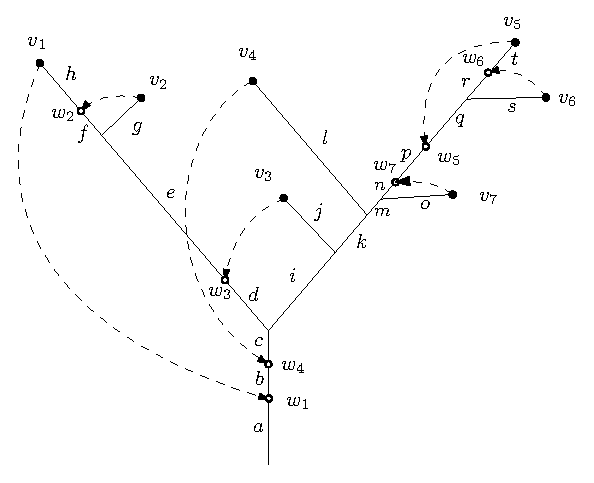
\includegraphics[width=0.8\linewidth]{Content/Pictures/out_componentswithmarks.eps}
    \caption{This is a subtree of an out-component spanned by the root of the out-component and the candidate tails $(v_1,\dots,v_7)$. Call the marked tree $T^{\mathrm{mk}}$. The heads of the candidates are denoted by $(w_1,\dots,w_7)$. }
\label{figure.extractSCCs1}
\end{subfigure}\\
\vspace{1.5em}
\begin{subfigure}{.8\textwidth}
  \centering
  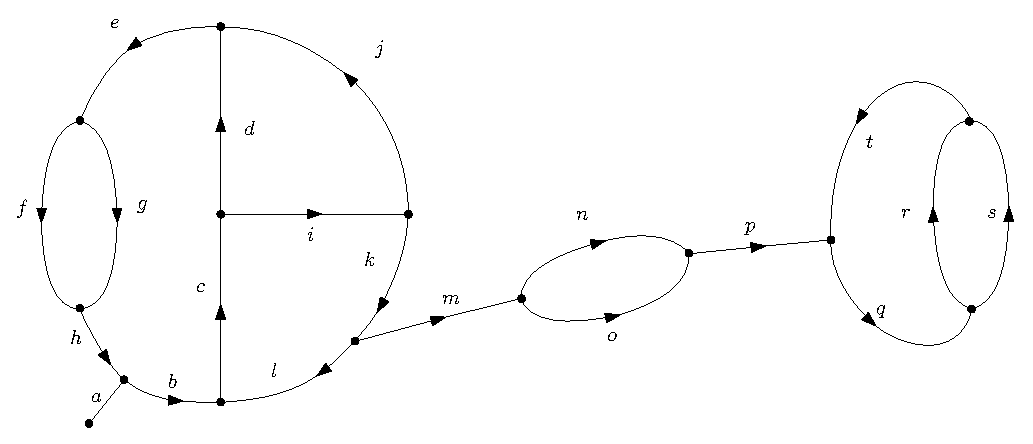
\includegraphics[width=0.9\linewidth]{Content/Pictures/identification.eps}
  \caption{Identifying $v_i$ with $w_i$ for $i\in [7]$ gives $M$.}
  \label{figure.extractSCCs2}
\end{subfigure}\\
\vspace{1.5em}
\begin{subfigure}{.8\textwidth}
  \centering
  \includegraphics[width=0.9\linewidth]{Content/Pictures/cutting.eps}
  \caption{We find the SCCs that are contained in $M$.}
  \label{figure.extractSCCs3}
\end{subfigure}

\caption{We illustrate the procedure to find the SCCs in a component of the out-forest after finding the candidates. Taken from \cite{goldschmidtScalingLimitCritical2019} with permission of the authors.}
\end{figure}

\subsection{The continuum case}\label{subsec.limitobject}

We will define now define the continuous counterpart of the sampling procedure of the out-forest and the candidates. This is a modification of the procedure defined in Subsection 3.2.2 of \cite{goldschmidtScalingLimitCritical2019}.

\subsubsection{\texorpdfstring{$\R$}{R}-trees and their encoding}
\input{Content/Sections/Real_Trees.tex}

\subsubsection{The limit object}\label{subsubsec.samplecontinuousobject}
Let $(B_t,t\geq 0)$ be a Brownian motion, and set $$\left(\hat{B}_t,t\geq 0\right)=\left(B_t-\frac{\sigma_{-+}+\nu_-}{2\sigma_+\mu}t^2,t\geq 0\right).$$ 
\begin{remark}
We note that the coefficient of the parabolic drift is negative. Indeed, the sign of the parabolic drift is the same as the sign of $\mu-\E[(D^-)^2D^+]$, and we note that
$$\frac{\E[(D^-)^2D^+]}{\E[D^+]}-\left(\frac{\E[D^+D^-]}{\E[D^+]}\right)^2=\frac{\E[(Z^+)^2]}{\mu}-1$$
is the variance of $D^-$ under the law of $\mathbf{D}$ size-biased by $D^+$, which is positive. Hence $\E[D^+(D^-)^2]/\mu\geq 1$, which shows that $(\hat{B}_t)_{t\geq 0}$ is a Brownian motion with a downwards parabolic drift.
\end{remark}
Define 
$$(\hat{R}_t,t\geq 0)= \left(\hat{B}_t-\inf\left\{\hat{B}_s: s\leq t\right\},t\geq 0\right).$$
Then, it is standard that $\left(\frac{2}{\sigma_+}\hat{R}_t,t\geq 0\right)$ is the height process corresponding to an $\R$-forest with \L ukasiewicz path $\left(\sigma_+\hat{B}_t,t\geq 0\right)$.  This fact also follows from the argument in Section \ref{sec.convoutforest}. Call this forest $(\hat{\cF}(t),t\geq 0)$. \\
Let $(A_t,t\geq 0)$ be a Cox process of intensity $$\frac{2(\sigma_{-+}+\nu_-)}{\sigma_+\mu^2} \hat{R}_t$$ at time $t$. Then, fix $T>0$, so that $A_T<\infty$ almost surely. For $i$ in $\left[A_T\right]$, set $X_i=\min\{t:A_T=i\}$. Define
\begin{align*}
L_i&=\inf\left\{t\geq 0:=\hat{B}_t=\inf\{\hat{B}_s:s\leq X_i\}\right\}\text{ for }i\in \left[A_T\right]\text{ and}\\
\Sigma_i&=\inf\left\{ t\geq 0: \inf\{\hat{B}_s:s\leq L_i+t\} < \inf\{\hat{B}_s:s\leq X_i\}\right\}\text{ for }i\in \left[A_T\right],
\end{align*}
so that for each $i$ in $\left[A_T\right]$, $\left(\frac{2}{\sigma_+}\hat{R}_t,t\in [L_i,L_i+\Sigma_i]\right)$ encodes the $\R$-tree in $(\hat{\cF}(t),t\geq 0)$ that contains $X_i$. For each element of $\{(L_i,\Sigma_i):i\in A_T\}$ we will sample the candidates in the $\R$-tree. Fix $i$, and set $(l,\sigma)=[L_i,\Sigma_i]$. Let $V_1=\inf\{s>0:A(s)=A(l)+1\}$, so that $l\leq V_1\leq l+\sigma$ by definition of $(l,\sigma)$. Let $\cT_l$ be the $R$-tree encoded by $\left(\frac{2}{\sigma_+}\hat{R}_t,t\in [l,l+\sigma]\right)$ and let $p_l:[l,l+\sigma]\to \cT_l$ be the projection onto $\cT_l$ given by the encoding. Set $$||\cT_l||=\sup\left\{\frac{2}{\sigma_+}\hat{R}_t,t\in [l,l+\sigma]\right\},$$
which we note is the height of $\cT_l$. \\
Suppose we have found candidates $\{V_1,\dots,V_m\}$. For $V_m\leq s\leq l+\sigma$, let $T^{\mathrm{mk}}_s$ be the subtree of $\cT_l$ spanned by $p_l\left(\{l,V_1,\dots,V_m,s\}\right)$, and let $|T^{\mathrm{mk}}_s|$ be its total length. Then, let $V_{m+1}$ be the first arrival time of a Poisson process on $[V_m,l+\sigma]$ of intensity $$\frac{\sigma_{-+}+\nu_-}{\mu^2}|T^{\mathrm{mk}}_s|ds.$$ If the process does not contain a point, let $\{V_1,\dots,V_m\}$ be the candidates of $\cT_l$, and set $N=m$. Otherwise, we repeat the inductive step for $\{V_1,\dots,V_{m+1}\}.$ If the induction does not terminate, we set $N=\infty$.\\
We show that $\P(N=\infty)=0$, by adapting the argument in Subsection 3.2.2 of \cite{goldschmidtScalingLimitCritical2019} to our set-up. Indeed, note that $V_m\leq s\leq V_{m+1}$ implies that  $|T^{\mathrm{mk}}_s|<(m+1)||\cT_l||$. Therefore, 
$$\P\left(\left.N\geq l+1,V_{m+1}-V_m<t \right|N\geq l\right)\leq \P(E_{m+1}<t),$$
for $(E_{k},k\geq 1)$ a sequence of exponential random variables with respective rates $$\frac{\sigma_{-+}+\nu_-}{\mu^2}k||\cT_l||.$$ 
Then,
$$\P\left(N=\infty \right)=\P\left(N=\infty\text{ and }\sup\{c_i:i\in \N\}<l+\sigma\right)\leq \P\left(\sum_{i=2}^\infty E_k\leq l+\sigma-V_1\right).$$
However, $\sum_{i=2}^\infty E_k=\infty$ a.s., because the harmonic series diverges, so, indeed, $\P\left(N<\infty \right)=1$. \\
Finally, for $1\leq i \leq N$, let the head corresponding to $V_i$, which we call $W_i$, be a uniform pick from the length measure on $T^{\mathrm{mk}}_{V_i}$. \\
Let $T^{\mathrm{mk}}(l)$ be the subtree of $\cT^{l}$ spanned by $\{l,V_1,\dots,V_N\}$. Then, in $T^{\mathrm{mk}}(l)$, set $V_i\sim W_i$ for each $1\leq i\leq N$, and set $\cM_{l}:=T^{\mathrm{mk}}(l)/\sim$. View $\cM_{l}$ as an element of $\vec{\cG}$ in the natural way. To be precise,  let the vertex set of $\cM_l$ consist of $l$, $W_i$ for $i\leq N$, and the branch points $V_i\wedge V_j$ for $i\neq j\leq N$. The directions are inherited from $\cT^l$, by considering all edges directed away from the root. Remove all edges that do not lie in an SCC of $\cM_{l}$ and delete any isolated vertices that are thus created. Then, apply the smoothing operation as defined in Subsection \ref{subsec.mdmkernels}. This creates a collection $\cC_l$ of strongly connected MDMs. Doing this for each $(l,\sigma)\in \{[L_i,\Sigma_i]\}$ yields the collection of strongly connected MDMs $\cC$ that has the law of the limit in Theorem \ref{thm.main}.

\subsubsection{Properties of the limit object}
We note that the limit object is encoded by $3$ parameters: the real forest is encoded by a Brownian motion with variance $\sigma_+^2$ and parabolic drift with coefficient $-(\sigma_{-+}+\nu_-)/(2\mu)$, and the identifications are a Cox process with intensity $(\sigma_{-+}+\nu_-)/\mu^2$ on the length measure of the subtree spanned by the previously found candidates and the currently explored point as described in \ref{subsubsec.samplecontinuousobject}. The limit object that is studied in \cite{goldschmidtScalingLimitCritical2019} corresponding to $\lambda=0$ (i.e. at criticality) is equal to our limit object in the case $\sigma_+^2=1$, $-(\sigma_{-+}+\nu_-)/(2\mu)=-1/2$, and $(\sigma_{-+}+\nu_-)/(\mu^2)=1$. Note that these three conditions are satisfied if we let $D^-$ and $D^-$ be independent $\operatorname{Poisson}(1)$ random variables. In \cite{goldschmidtScalingLimitCritical2019}, some properties of the limit object corresponding to these specific parameters are shown. A quick check shows that the proofs do not depend on the values of the parameters, so we deduce that the properties also hold for our limit object. Let $\cM:=\bigcup_{L_i}\cM_{L_i}$.

\begin{corollary}
\begin{enumerate}
    \item The number of complex connected components of $\cM$ has finite expectation.
    \item The number of loops of $\cM$ is a.s. finite.
\end{enumerate}
\end{corollary}
\begin{proof}
The proof is analogous to the proof of Theorem 4.5 in \cite{goldschmidtScalingLimitCritical2019}.
\end{proof}
\begin{corollary}\label{cor.allengthsaredifferent}
The SCCs of $\cM$ all have different lengths almost surely.
\end{corollary}
\begin{proof}
The proof is analogous to the proof of Proposition 4.6 in \cite{goldschmidtScalingLimitCritical2019}.
\end{proof}
Write $\cC$ for the SCCs of $\cM$ and $\mathbf{C}_l$ for those of $\cM_l$, in decreasing order of length, with $\cM_l$ as defined in Subsection  \ref{subsubsec.samplecontinuousobject}. Write $\cC_{\text{cplx}}$ for the list of complex components of $\cC$ in decreasing order of length. For sequences $(K_1,\dots, K_j)$ and $(J_1,\dots,J_k)$ of directed multigraphs, write $(J_1,\dots,J_k)\equiv(K_1,\dots, K_j)$ if $j=k$ and $J_i$ is isomorphic to $K_i$ for each $i\leq j$. Extend this notation naturally to the case where one or both of the sequences has edge lengths by ignoring the edge lengths. 
\begin{corollary}
Let $K_1,\dots, K_j$ be a finite sequence consisting of $3$-regular strongly connected directed multigraphs or loops. We have 
$$\P\left[\cC_l\equiv(K_1,\dots, K_j)\right]>0.$$
Assuming that $K_1,\dots, K_j$ are all complex, we also have that 
$$\P\left[ \cC_{\text{cplx}}\equiv(K_1,\dots, K_j)\right]>0.$$
Let $(e_i,1\leq i \leq K)$ be an arbitrary ordering of the edges of $K_1,\dots, K_j$. Then, conditionally on $\cC_l\equiv(K_1,\dots, K_j)$, (resp. $\cC_{\text{cplx}}\equiv(K_1,\dots, K_j)$), $\cC_l$ (resp. $\cC_{\text{cplx}}$) gives lengths $(\ell(e_i),1\leq i \leq K)$ to these edges, and their joint distribution has full support in 
$$\left\{\mathbf{x}=(x_1,\dots, x_K)\in \R_+^K:\forall 1\leq i\leq k-1, \sum_{j:e_j\in E(K_i)}x_j \geq \sum_{j:e_j\in E(K_{i+1})}x_j\right\}.$$
\end{corollary}
\begin{proof}
The proof is analogous to the proof of Theorem 6.1 in \cite{goldschmidtScalingLimitCritical2019}.
\end{proof}


\input{Content/Sections/Measure_change}
\section{Convergence of the out-forest}\label{sec.convoutforest}
 Fix $T>0$. In this section we will show that the \L ukasiewicz path and height process corresponding to the out-forest converge under rescaling up to time $\lfloor T n^{2/3}\rfloor$. Note that the out-forest will contain at least $n$ vertices, so for $n$ large enough, $\lfloor T n^{2/3}\rfloor\leq n$ and the encoding processes are well-defined up to time $\lfloor T n^{2/3}\rfloor$. 
 
We will show that the convergence under rescaling of the \L ukasiewicz path and height process $(\hat{S}^{+}_n(k),\hat{H}_n(k),k\leq \lfloor Tn^{2/3}\rfloor)$ occurs jointly with convergence in distribution under rescaling of $(\hat{S}^-_n(k),\hat{P}_n(k), k\leq \lfloor Tn^{2/3}\rfloor)$, for $\hat{S}^-_n(k)$ the number of unpaired in-half-edges of vertices that have been discovered at time $k$, and $\hat{P}_n(k)$ the number of dummy leaves added in the first $k$ time-steps.  \\
We let $(B_t)_{t\geq 0}$ be a Brownian motion, and define
$$(\hat{B}_t,t\geq 0):=\left( B_t-\frac{\sigma_{-+}+\nu_-}{2\sigma_+ \mu}t^2, t\geq 0\right).$$ 
We define the reflected process $$(\hat{R}_t,t\geq 0)= \left(\hat{B}_t-\inf\left\{\hat{B}_s: s\leq t\right\},t\geq 0\right).$$

The main result of this section is as follows. 

\begin{proposition}\label{prop:convoutforest}
It holds that
\begin{align*}\left(n^{-1/3}\hat{S}^{+}_n\left(\lfloor n^{2/3}t\rfloor \right),n^{-1/3}\hat{H}_{n}\left(\lfloor n^{2/3}t\rfloor \right), t\leq T \right)
\todist\left(\sigma_+ \hat{B}_t, \frac{2}{\sigma_+} \hat{R}_t, t\leq T \right)\end{align*}
in $\D([0,T],\R)^2$, and 
\begin{align*}\left( n^{-2/3}\hat{S}_n^-\left(\lfloor n^{2/3}t\rfloor \right), n^{-1/3}\hat{P}_n\left(\lfloor n^{2/3}t\rfloor \right), t\leq T \right)\toprob\left(\nu_-t,  \frac{\nu_-}{2\mu} t^2, t\leq T \right)\end{align*}
in $\D([0,T],\R)^2$ as $n\to \infty$. 
\end{proposition}
We prove \cref{prop:convoutforest} by studying two other forests that are related to the out-forest via a change of measure.  \\
The proof is structured as follows.
\begin{enumerate}
    \item \label{item.measurechangeexists} Recall that $(\mathbf{\widehat{D}}_{n,1},\dots,\mathbf{\widehat{D}}_{n,n})$ are the degree pairs of the vertices in order of discovery. Also recall $\mathbf{Z}_1, \mathbf{Z}_2, \ldots$ in an i.i.d.\ sequence of $\N\times \N$-valued random variables, $\mathbf{Z}_i:=(Z_i^-,Z_i^+)$, such that 
    $$\P(Z_i^-=k^-, Z_i^+=k^+)=\frac{k^-\P(D^-=k^-,D^+=k^+)}{\mu}.$$
    In \cref{sec:measure-change}, we showed that the law of $(\mathbf{\widehat{D}}_{n,1},\dots,\mathbf{\widehat{D}}_{n,m})$ conditional on $\sum_{i=1}^n D_i^-=\sum_{i=1}^n D_i^+$ and $m \leq R_n$ is absolutely continuous with respect to that of $(\mathbf{Z}_1,\dots, \mathbf{Z}_m)$, and we showed the convergence under rescaling of the Radon-Nikodym derivative $\phi_m^n$ for $m=\lfloor T n^{2/3}\rfloor$. 
    \item Point \ref{item.measurechangeexists} motivates us to study a Bienaymé forest with offspring distributed as $Z_1^+$. The convergence of the \L ukasiewicz path of this forest under rescaling follows from Donsker's theorem.
    \item In Subsection \ref{subsec.purpleleavesGWforest}, we modify the Bienaymé forest in order to include dummy leaves. We add extra randomness, approximating the procedure described in \cref{prop:sampleoutforest}, in such a way that at some time-steps, a dummy leaf is added. We call the resulting forest \emph{the forest with dummy leaves}. We respect the order of the degrees in the Bienaymé forest, in the sense that for any $k$, the $k$th true vertex in the forest with dummy leaves has the same number of children as the $k$th vertex in the Bienaymé forest. The law of the forest with dummy leaves depends on $n$, because the probability of finding a dummy leaf depends on $n$. We then show that the \L ukasiewicz path and height process of the forest with dummy leaves converge under rescaling, jointly with the convergence of the \L ukasiewicz path and height process of the Bienaymé forest under rescaling up to time $\lfloor T n^{2/3}\rfloor$.
    \item We show convergence under rescaling of the out-forest up to time $\lfloor T n^{2/3}\rfloor$ by applying the measure change to the forest with dummy leaves and showing that the resulting forest is a good approximation of the out-forest. 
\end{enumerate}

\subsection{Convergence before adding the dummy leaves}
We define the two processes
$$ \hat{Y}^{\pm}(k)=\sum\limits_{i=1}^k (\widehat{D}^{\pm}_{n,i}-1), $$
for $1\leq k\leq n$, which encode the degrees in order of discovery.

We will study these processes via the measure change that we defined in \cref{sec:measure-change}. Let
\begin{equation*}
  Y^{\pm}(k) = \sum_{i=1}^k (Z_i^{\pm} - 1)
\end{equation*}
be the corresponding walks for $(\vZ_i)_{i=1}^{\infty}$. Then, in the critical case, these are related to the centered random walks $V^{\pm}$ by
\begin{equation*}
  Y^+(k) = V^+(k)
  \quad \text{and} \quad
  Y^-(k) = V^-(k) - (\lambda_- - 1) k = V^-(k) - \nu_- k.
\end{equation*}
Therefore, we obtain the following corollary of \cref{prop:measure-change-no-crit}.
\begin{corollary}
  \label{cor:measure-change}
  Suppose we are in the setting of \cref{prop:measure-change-no-crit} and that the criticality condition holds. Then for all $T > 0$,
  \begin{align*}
      &\left( 
          \Phi(n, \floor{n^{2/3} T}),
          \left(
              n^{-1/3} V^-\left( \floor{n^{2/3} t} \right),
              n^{-1/3} V^+\left( \floor{n^{2/3} t} \right)
          \right)_{t \in [0, T]}
      \right) \\
      & \hspace{23em} \todist \left( 
          \Phi(T),
          (\sigma_- W^+_t, \sigma_+ W^+_t)_{t \in [0, T]}
      \right)
  \end{align*}
  in $\R \times \D([0, T], \R^2)$ as $n \to \infty$ and $\left(\Phi(n,\floor{n^{2/3} T})\right)_{n\geq 1}$ is uniformly integrable.
\end{corollary}
Let $(\hat{B}_t,t\geq 0)$ be distributed as follows. For $F$ a suitable test function, and for $(B_t)_{t\geq 0}$ a Brownian motion,
\begin{align*} &\E\left[F(\sigma_+ \hat{B}_t,0\leq t \leq T)\right]\\&=\E\left[\exp\left(-\frac{\sigma_{-+}}{\sigma_+ \mu} \int_0^T s dB_s -\frac{\sigma_{-+}^2 T^3}{6\sigma_+^2 \mu^2}\right)F(\sigma_+ B_t,   0\leq t \leq T)\right].\end{align*}

 
%  Recall that 
%  $$ {Y}^+(k)=\sum\limits_{i=1}^k (Z^+_i-1),$$ 
%  and 
%  $$ {Y}^-(k)=\sum\limits_{i=1}^k (Z^-_i-1).$$ 
%  Then, Donsker's theorem and the law of large numbers imply the following straightforward lemma.
% \begin{lemma}
% \label{lem.jointconvergenceinout}
%  We have $$ \left(n^{-2/3}{Y}^-\left(\lfloor n^{2/3}t\rfloor\right), t\geq 0\right)
%  \toprob 
%  \left(\nu_-t, t\geq 0 \right)$$
%  in $\D(\R_+,\R)^2$ as $n\to \infty$.  Moreover,
%  \begin{align*} &\left(n^{-1/3}\left({Y}^-\left(\lfloor n^{2/3}t\rfloor\right)-n^{2/3}\nu_-t\right),n^{-1/3}Y^+\left(\lfloor n^{2/3}t\rfloor\right), t\geq 0\right)\\
%  &\todist 
%  \left(\mathbf{B}_t, t\geq 0 \right)\end{align*}
%  in $\D(\R_+,\R)^2$, as $n\to \infty$, with $(\mathbf{B}_t,t\geq 0)$ a Gaussian process with covariance matrix
%  $$\begin{pmatrix} \sigma_-^2  & \sigma_{-+} \\ \sigma_{-+}  & \sigma_+^2  \end{pmatrix}t.$$
% \end{lemma} 

\begin{proposition}\label{prop:convaftermeasurechange} 
 We have that
$$\left(n^{-2/3}\hat{Y}^-\left(\lfloor n^{2/3} t\rfloor\right), n^{-1/3}\hat{Y}^+\left(\lfloor  n^{2/3} t\rfloor\right), 0\leq t \leq T \right) \todist \left( \nu_- t, \sigma_+\hat{B}_t, 0 \leq t \leq T \right)$$
in the Skorokhod topology as $n\to \infty$.
\end{proposition}
\begin{proof}
 We recall from the statement of \cref{cor:measure-change} that $(W^-,W^+)$ is a pair of correlated standard Brownian motions with correlation $\operatorname{Corr}(Z_1^-,Z_1^+)$. 
Let $(B^1_t,t\geq 0)$ and $(B^2_t,t\geq 0)$ be two independent Brownian motions, so that we may define $$(\sigma_-W^-_t,\sigma_+W^+_t,t\geq 0)=\left(\frac{\sigma_{-+}}{\sigma_+}B_t^1+\left(\sigma_-^2-\frac{\sigma_{-+}^2}{\sigma_+^2}\right)^{1/2} B_t^2, \sigma_+ B_t^1, t\geq 0\right).$$ 
 Then, \cref{cor:measure-change} implies that for $F$ a continuous, bounded test function, 
 \begin{align*}&\E\left[F\left(n^{-1/3}\hat{Y}^+\left(\lfloor n^{2/3}t\rfloor\right), 0\leq t \leq T \right) \right]\\
 &=\E\left[F\left(n^{-1/3}\hat{Y}^+\left(\lfloor n^{2/3}t\rfloor\right), 0\leq t \leq T \right)\one_{\lfloor Tn^{2/3}\rfloor \leq R_n} \right]+o(1)\\
 &= \E\left[\Phi(n,\floor{n^{2/3}T})F\left(n^{-1/3}{V}^+\left(\lfloor n^{2/3}t\rfloor\right), 0\leq t \leq T \right) \right]+o(1).\end{align*}
By the proof of Proposition \ref{prop:measure-change-no-crit}, we see that for $$\Gamma(n,m)=\exp\left(\frac{1}{\mu n} \sum_{i=0}^m(V^-(i)-V^-(m))-\frac{\sigma_-}{6\mu^2}\frac{m^3}{n^2}\right),$$
we have that 
$$\E\left[\left|\Phi(n,\lfloor n^{2/3}T\rfloor)-\Gamma(n,\lfloor n^{2/3}T\rfloor)\right|\right]\to  0$$
as $n\to\infty$, so it sufficient to show that 
$$\E\left[ \Gamma(n,\lfloor n^{2/3}T\rfloor)F\left(n^{-1/3}V^+\left(\lfloor n^{2/3}t\rfloor\right), 0\leq t \leq T \right)\right] \to \E\left[F\left(\sigma_+\hat{B}_t,0\leq t\leq T\right)\right].$$
Write 
$V^+_{(n)}(t)=n^{-1/3}{V}^+\left(\lfloor n^{2/3}t\rfloor\right)$ and $V^-_{(n)}(t)=n^{-1/3}V^-\left(\lfloor n^{2/3}t\rfloor\right)$. 
Then we observe that 
 $$\Gamma(n,\floor{n^{2/3}T})=\exp\left(\frac{1}{\mu}\int_0^T\left({V}^-_{(n)}(t)-{V}^-_{(n)}(T)\right)dt-\frac{\sigma_-}{6\mu^2}\frac{\lfloor Tn^{2/3}\rfloor^3}{n^2}\right).$$
For a path $x\in \D([0,T],\R)$, let 
$$\Theta(x,T)= \exp\left(\frac{1}{\mu}\int_0^T\left(x(t)-x(T)\right)dt-\frac{\sigma_-}{6\mu^2}T^3\right)$$
so that $\Theta$ is a continuous functional of its first argument and 
$$\E\left[\left|\Gamma(n,\floor{n^{2/3}T})-\Theta({V}^-_{(n)} ,T)\right|\right]\to 0$$
as $n\to\infty$. This implies that it suffices to show that 
$$\E\left[\Theta({V}^-_{(n)} ,T)F\left(V^+_{(n)}(t), 0\leq t \leq T \right)\right] \to \E\left[F\left(\sigma_+\hat{B}_t,0\leq t\leq T\right)\right].$$
But, by the continuity of $\Theta$ and Corollary \ref{cor:measure-change}, we get that 
\begin{align*}&\E\left[\Theta({V}^-_{(n)} ,T)F\left(V^+_{(n)}(t), 0\leq t \leq T \right)\right]\to \E\left[\Theta(\sigma_- W_t^- ,T)F\left(\sigma_+W_t^+, 0\leq t \leq T \right)\right]\\
&\qquad=\E\left[\exp\left(-\frac{1}{\mu}\int_0^Tsd\left(\frac{\sigma_{-+}}{\sigma_+}B_s^1+\left(\sigma_-^2-\frac{\sigma_{-+}^2}{\sigma_+^2}\right)^{1/2}B_s^2\right) - \frac{T^3 \sigma_-^2}{6\mu^2}\right) F\left(\sigma_+ B_t^1, 0\leq t \leq T\right)\right]\\
 &\qquad=\E\left[\exp\left(-\frac{\sigma_{-+}}{\sigma_+ \mu} \int_0^T s dB^1_s -\frac{\sigma_{-+}^2 T^3}{6\sigma_+^2 \mu^2}\right)F(\sigma_+ B^1_t,   0\leq t \leq T)\right].\end{align*}




%  {\color{red}UNFINISHED, I will continue here}
 % Then, by the proof of Proposition \ref{prop:measure-change-no-crit}, we see that for $$\Gamma(n,m)=\exp\left(\frac{1}{\mu n} \sum_{i=0}^m(Y^-(i)-Y^-(m)+\nu_-(m-i))-\frac{\sigma_-}{6\mu^2}\frac{m^3}{n^2}\right),$$
% we have that 
% $$\E\left[\left|\Phi(n,m)-\Gamma(n,m)\right|\right]\to  0$$
% as $n\to\infty$, so it sufficient to show that 
% $$\E\left[ \Gamma(n,m)f\left(V^+_{(n)},S^+_{(n)},  H^+_{(n)}\right)\right] \to \E\left[\Phi(T)f\left(\sigma_+ W^+_t,\sigma_+ B^+_t,\frac{2}{\sigma_+}R^+_t,0\leq t \leq T\right)\right].$$
% Then we observe that 
% $$\Gamma(n,m)=\exp\left(\frac{1}{\mu}\int_0^T\left({V}^-_{(n)}(t)-{V}^-_{(n)}(T)\right)dt-\frac{\sigma_-}{6\mu^2}\frac{\lfloor Tn^{2/3}\rfloor^3}{n^2}\right).$$
% Therefore, for a path $x\in \D([0,T],\R)$, let 
% $$\Theta(x,T)= \exp\left(\frac{1}{\mu}\int_0^T\left(x(t)-x(T)\right)dt-\frac{\sigma_-}{6\mu^2}T^3\right)$$
% so that $\Theta$ is a continuous functional of its first argument and 
% $$\E\left[\left|\Gamma(n,m)-\Theta({V}^-_{(n)}(t) ,T)\right|\right]\to 0$$
% as $n\to\infty$. 
% Therefore, it suffices to show that 
% $$\E\left[ \Theta({V}^-_{(n)}(t) ,T)f\left(V^+_{(n)},S^+_{(n)},  H^+_{(n)}\right)\right] \to \E\left[\Theta(W^- ,T)f\left(\sigma_+ W^+_t,\sigma_+ B^+_t,\frac{2}{\sigma_+}R^+_t,0\leq t \leq T\right)\right].$$
 
%  \\\to& \E\left[\exp\left(-\frac{1}{\mu}\int_0^Tsd\left(\frac{\sigma_{-+}}{\sigma_+}B_s^1+\left(\sigma_-^2-\frac{\sigma_{-+}^2}{\sigma_+^2}\right)^{1/2}B_s^2\right) - \frac{T^3 \sigma_-^2}{6\mu^2}\right) F\left(\sigma_+ B_t^1, 0\leq t \leq T\right)\right]\\
%  &=\E\left[\exp\left(-\frac{\sigma_{-+}}{\sigma_+ \mu} \int_0^T s dB^1_s -\frac{\sigma_{-+}^2 T^3}{6\sigma_+^2 \mu^2}\right)F(\sigma_+ B^1_t,   0\leq t \leq T)\right].\end{align*}
%  For the details of the argument, we refer the reader to the proof of Theorem 4.1 in \cite{conchon--kerjanStableGraphMetric2021}.
 Then, the fact that $(Y(k),k\geq 1)$ is a random walk with steps of mean $\nu_-$ implies that
 $$\left(n^{-2/3}Y^-\left(\lfloor n^{2/3}t\rfloor\right),t\geq 0\right)\toprob\left(\nu_- t,t\geq 0\right),$$
 and then, by repeating the argument above, noting that the change of measure does not affect the deterministic process $(\nu_- t,t\geq 0)$, also 
 $$\left(n^{-2/3}\hat{Y}^-\left(\lfloor n^{2/3}t\rfloor\right),t\geq 0\right)\toprob\left(\nu_- t,t\geq 0\right),$$
 which proves the statement.
 \end{proof}
 The following proposition characterises the distribution of $(\hat{B}_t, {0\leq t\leq T})$.
 \begin{proposition}
 \label{prop:characterizelimitprocess}
 We have that
 $$(\sigma_+ \hat{B}_t, {0\leq t\leq T})\overset{d}{=}\left(\sigma_+ B_t-\frac{\sigma_{-+}}{2\mu}t^2, {0\leq t\leq T}\right),$$
 where $(B_t)_{t\geq 0}$ is a standard Brownian motion.
 \end{proposition}
 \begin{proof}
 Firstly, we have that for any $t\in [0,T]$ and $\theta>0$,
 \begin{align*} \E\left[\exp(-\theta \sigma_+ \hat{B}_t)\right] &= \E \left[ \exp\left(-\frac{\sigma_{-+}}{\sigma_+ \mu}\int_0^t s dB_s-\frac{\sigma_{-+}^2 t^3}{6\sigma_+^2\mu^2}-\theta\sigma_+ B_t  \right)\right]\\
 &=\E\left[\exp \left( -\frac{\sigma_{-+}}{\sigma_+ \mu}\int_0^t \left(s+\frac{\sigma_+^2\theta \mu}{\sigma_{-+}}\right) dB_s -\frac{\sigma_{-+}^2 t^3}{6\sigma_+^2\mu^2}\right)\right] \\
 &= \exp\left(-\frac{\sigma_{-+}^2}{2\sigma_+^2 \mu^2}\int_0^t \left(s+\frac{\sigma_+^2\theta \mu}{\sigma_{-+}}\right)^2 ds -\frac{\sigma_{-+}^2 t^3}{6\sigma_+^2\mu^2}\right)\\
 &=\exp\left(\frac{\sigma_+^2 t}{2}\theta^2+\frac{\sigma_{-+} t^2}{2\mu}\theta \right)\\
 &= \E \left[\exp\left(-\theta\left(\sigma_+ B_t - \frac{\sigma_{-+}}{2\mu} t^2\right)\right)\right].
 \end{align*}
 Then, more generally, for $m>0$, $0=t_0\leq t_1\leq \cdots \leq t_m=T$, and $\theta_1, \dots, \theta_m \in \R_+$, 
 \begin{align*}
     &\E\left[\exp\left(-\sum_{i=1}^m \theta_i(\sigma_+\hat{B}_{t_i}-\sigma_+\hat{B}_{t_{i-1}})\right)\right]\\
    %  &=\E \left[ \exp\left(-\frac{\sigma}{\mu} \sum_{i=1}^m \int _{t_{i-1}}^{t_i} s dB_s^1-\frac{\sigma_-^2}{2\mu^2}\sum_{i=1}^m \int_{t_{i-1}}^{t_i}s^2ds-\frac{ \sigma_{-+}}{\sigma} \sum_{i=1}^m \theta_i(B_{t_i}^1-B_{t_{i-1}}^1)- 
    %  \left(\sigma_+^2-\frac{\sigma_{-+}^2}{\sigma_-^2}\right)^{1/2}\sum_{i=1}^m \theta_i(B_{t_i}^2-B_{t_{i-1}}^2)\right)\right]\\
     &= \prod_{i=1}^m \E\left[\exp\left(-\frac{\sigma_{-+}}{\sigma_+\mu} \int _{t_{i-1}}^{t_i} s dB_s-\frac{\sigma_{-+}^2 (t_i^3-t_{i-1}^3)}{6\sigma_+^2 \mu^2}-\theta_i \sigma_+  (B_{t_i}-B_{t_{i-1}})\right)\right]\\
     &= \prod_{i=1}^m  \exp\left( -\frac{\sigma_{-+}^2}{2\sigma_+^2 \mu^2}\int_{t_{i-1}}^{t_i}\left(s+\frac{\sigma_+^2\theta_i\mu}{\sigma_{-+}}\right)^2 ds - \frac{\sigma_{-+}^2 (t_i^3-t_{i-1}^3)}{6\sigma_+^2 \mu^2} \right)\\
     &=  \prod_{i=1}^m \exp\left(\frac{ \sigma_+^2 (t_i-t_{i-1}) }{2}\theta_i^2+\frac{\sigma_{-+} (t_i^2-t_{i-1}^2)}{2\mu}\theta_i \right)\\
     &=\E \left[\exp\left(-\sum_{i=1}^m\theta_i\left(\sigma_+ (B_t-B_{t_i}) - \frac{\sigma_{-+}}{2\mu} (t_i^2-t_{i-1}^2)\right)\right)\right],
 \end{align*}
 which proves the result.
 \end{proof}
\subsection{Adding dummy leaves to a Bienaymé forest}\label{subsec.purpleleavesGWforest}
We would like to add dummy leaves to the forest encoded by $(Y^+(l),1\leq l \leq k)$. However, in the absence of a true stack of in-edges, we need to approximate the probability of adding a dummy leaf. We do this by approximating the stack size by its mean $\mu n$. 
% \begin{lemma}
% Consider an eDFS of a configuration model on $n$ vertices, with the total number of in-half-edges equal to $\mu n$. Suppose the number of unpaired in-half-edges of discovered vertices at step $k$ in the exploration is equal to $S_n^{-}(k)$, suppose $(S_n^{+}(l),1\leq l\leq k)$ encodes the \L ukasiewicz path of the out-forest up to time $k$, and set $$I_n^{+}(k)=\inf\left\{S_n^{+}(l),1\leq l\leq k\right\}.$$
% Then, the probability that, in the $(k+1)$th time-step, we sample a surplus edge is given by
% $$p_{k+1}:=\frac{S_n^{-}(k)}{\mu n - k -I^{+}(k)+1}\one_{\{I^{+}(k)=I^{+}(k-1)\}}.$$
% \end{lemma}
% \begin{proof}
% This is a slight adaptation of Lemma \ref{lemma.sampleoutforest}, with the sequence $(\mathbf{\widehat{D}}_{n,1},\dots,\mathbf{\widehat{D}}_{n,m})$ replaced by $(\mathbf{Z}_1,\dots, \mathbf{Z}_m)$, and the total number of in-edges replaced by its mean $\mu n$.
% \end{proof}
We use this idea to define the forest with dummy leaves and its \L ukasiewicz path $(S_n^{+}(k), k\geq 1)$ as a function of $(Y^-(k), Y^+(k) ,k\geq 1)$ and some extra randomness to decide at which time-steps we add a dummy leaf.
\begin{enumerate} 
    \item Set $P_n(1)=0$, $S_n^{+}(1)=Z_1^+-1$, $S_n^{-}(1)=Z_1^-$. 
    \item Suppose we are given $(P_n(l),S_n^{+}(l),S_n^{-}(l), 1\leq l \leq k)$. Define 
    $I^{+}(k)=\min\{S_n^{+}(l), l\leq k\}$. Then, with probability $$p_{k+1}:=\frac{S_n^{-}(k)}{\mu n - k -I^{+}(k)+1}\one_{\{I^{+}(k)=I^{+}(k-1)\}},$$ independent from everything else, set $P_n(k+1)=P_n(k)+1$. Otherwise, set $P_n(k+1)=P_n(k)$. 
    \item Set $$S_n^{+}(k+1)=Y^+(k+1-P_n(k+1))-P_n(k+1),$$ and $$S_n^{-}(k+1)=Y^-(k+1-P_n(k+1))-P_n(k+1)-I^{+}(k)+1.$$
\end{enumerate}
Let the forest with dummy leaves be the forest with \L ukasiewicz path $(S_n^{+}(k), k\geq 1)$ in which the $k$th vertex is a dummy leaf if and only if $P^n(k)-P^n(k-1)=1$. 
\subsubsection{Convergence of the \L ukasiewicz path}
To show the convergence of the \L ukasiewicz path corresponding to the forest with dummy leaves, we will first examine the limit of $(P_n(k), k\geq 1)$ under rescaling. We will first prove tightness, after which we will show convergence.


\begin{lemma}\label{lemma.tightnesssurplusedges}
 We have that, $$\left(n^{-1/3}P_n\left(\lfloor  n^{2/3}t\rfloor \right) \right)_{n\geq 1}$$ 
 is tight for all $t>0$.
 \end{lemma}
 \begin{proof}
Set $m=\lfloor  n^{2/3}t\rfloor$ and fix $\epsilon>0$. It is trivial that for any $k\leq m$, $$S^{-}(k)\leq \sum_{i=1}^k Z^-_i=Y^-(k)+k.$$ Moreover, $\mu n - k -I^{+}(l)+1>\mu n-k$.  Therefore, $$p_{k+1}\leq \frac{Y^-(k)+k}{\mu n - k}.$$
This upper bound is increasing in $k$. Consequently, conditional on $(Y^+(j),Y^-(j),j\geq 1),$ $n^{-1/3}P_n(m)$ is stochastically dominated by a binomial random variable with parameters  $m$ and $$\frac{Y^-(m)+m}{\mu n - m}\wedge 1.$$
Since $(Y^-(k)+k,k\geq 1)$ is a random walk with steps of finite mean, $\left(n^{-2/3}(Y^-(m)+m)\right)_{n\geq 1}$ is tight. Therefore,
$$\left(n^{1/3} \frac{Y^-(m)+m}{\mu n - m}\right)_{n\geq 1}$$ is tight, which implies that a binomial random variable with parameters  $m$ and $$\frac{Y^-(m)+m}{\mu n - m}\wedge 1$$
is tight. The statement follows.
\end{proof}
\begin{lemma}\label{lemma.convergenceQandP}
We have  
$$\left(n^{-1/3}P_n(\lfloor n^{2/3}t\rfloor), t \geq 0 \right)\toprob \left(\frac{\nu_-}{2\mu} t^2, t\geq 0 \right)$$
in $D(\R_+,\R)$ as $n\to \infty$.

\end{lemma}
\begin{proof}
Recall that
$$p_{k+1}=\frac{S_n^{-}(k)}{\mu n - k -I^{+}(k)+1}\one_{\{I^{+}(k)=I^{+}(k-1)\}}.$$
Define $M^+(k)=\min\{Y^+(l):l\leq k\}$ so that $0\geq I^{+}(k)\geq M^+(k)-P_n(k)$.  Then, by Lemma \ref{lemma.tightnesssurplusedges}, the convergence under rescaling of $Y^+$ shown in \cref{cor:measure-change}, and the continuous mapping theorem, $\left(n^{-1/3}I^+(\lfloor n^{2/3} t \rfloor)\right)_{n\geq 1}$ is tight for all $t\geq 0$.
We will now argue that the indicator, which ensures that the roots are never dummy leaves, does not have an effect on $(P_n(k),k\leq m)$ on the scale of interest. Let $m=\lfloor n^{2/3}t\rfloor$. Define
\begin{align*}\begin{split}
E^p(m)&:=\sum_{k=0}^{m-1}\frac{S_n^{-}(k)}{\mu n - k -I^{+}(k)+1}\one_{\{I^{+}(k)\neq I^{+}(k-1)\}}\\
&\leq -I^{+}(m) \frac{Y^-(m)+m}{\mu n - m},\end{split}\end{align*}
so since $I^{+}(m)$ is of order $n^{1/3}$ and $\frac{Y^{-}(m)+m}{\mu n - m}$ is of order $n^{-1/3}$, $(E^p(m))_{n\geq 1}$ is tight.  This means that if we allow the roots to be dummy leaves, with high probability, we would only sample $O(1)$ roots that are dummy leaves up to time $O(n^{2/3})$. This does not affect $(P_n(k),k\leq m)$ on the scale of interest. \\
 Then, the convergence under rescaling of $Y^-$ and $Y^+$ shown in \cref{cor:measure-change}, the tightness of $\left(n^{-1/3}I^{+}(\lfloor n^{2/3} t \rfloor)\right)_{n\geq 1}$ and Lemma \ref{lemma.tightnesssurplusedges} imply that
\begin{align}\begin{split}\label{eq.convergenceprob}
  &\left(n^{1/3}\frac{S_n^{-}\left(\lfloor n^{2/3} t \rfloor\right)}{\mu n - \lfloor n^{2/3} t \rfloor -I^{p,+}\left(\lfloor n^{2/3} t \rfloor\right)+1},t\geq 0\right)\\
 &=\left(n^{1/3}\frac{Y^-\left(\lfloor n^{2/3} t \rfloor-P_n\left(\lfloor n^{2/3} t \rfloor\right)\right)-P_n\left(\lfloor n^{2/3} t \rfloor\right)-I^{+}\left(\lfloor n^{2/3} t \rfloor\right)+1}{\mu n - \lfloor n^{2/3} t \rfloor -I^{+}\left(\lfloor n^{2/3} t \rfloor\right)+1},t\geq 0\right)\\
 &\toprob \left(\frac{\nu_-}{\mu}t,t\geq 0\right)\end{split}\end{align}
in $D(\R_+,\R)$ as $n\to \infty$. 
Then, by the continuous mapping theorem and the tightness of $(E^p(m))_{n\geq 1}$,
$$\left(n^{-1/3}\sum_{i=0}^{\lfloor n^{2/3}t \rfloor} p_k , t \geq 0\right)\toprob \left(\frac{\nu_-}{2\mu}t^2,t\geq 0\right)$$
in $D(\R_+,\R)$ as $n\to \infty$. \\
Let $\cG=(\cG_k,k\geq 1)$ denote the filtration such that $\cG_{k}$ contains the information on the shape of the forest until time $k$, including which of the first $k$ vertices are dummy vertices. Then, 
$$M_n(k):=\sum_{i=1}^k (\one_{\{P_n(i)-P_n(i-1)=1\}}-p_i)$$ is a $\cG$-martingale. We claim that $(n^{-1/3}M_n(\lfloor n^{2/3} t\rfloor ), t\geq 0)$ converges to $0$ in probability in $D(\R_+,\R)$. Indeed, for any $t\geq 0$,
\begin{align*}\E[n^{-2/3}M_n(\lfloor n^{2/3} t\rfloor )^2]&=n^{-2/3}\sum_{i=1}^{\lfloor n^{2/3} t\rfloor} \E[\E[(\one_{\{P_n(i)-P_n(i-1)=1\}}-p_i)^2|\cG_{i-1}]]\\&=n^{-2/3}\sum_{i=1}^{\lfloor n^{2/3} t\rfloor} \E[p_i-p_i^2]\to 0.\end{align*}
Hence, since for all $t\geq 0$,
\begin{align*}n^{-1/3}P_n(\lfloor n^{2/3}t\rfloor)&=n^{-1/3}\sum_{i=1}^{\lfloor n^{2/3}t\rfloor}  \one_{\{P_n(i)-P_n(i-1)=1\}}\\
&= n^{-1/3}\sum_{i=0}^{\lfloor n^{2/3}t \rfloor} p_k + n^{-1/3} M_n\left(\lfloor n^{2/3}t\rfloor\right),
\end{align*}
we have
$$\left(n^{-1/3}P_n(\lfloor n^{2/3}t\rfloor),t\geq 0\right)\todist  \left( \frac{\nu_-}{2\mu}t^2, t\geq 0 \right),$$
 which proves the statement.

\end{proof}

The convergence of $P_n$ under rescaling implies the convergence of $S^{+}_n$ and $S^{-}_n$ under rescaling, which is the content of the following lemma. Let $(B_t,t\geq 0)$ be a Brownian motion, and define 
$$({B}^{\mathrm{d}}_t,t\geq 0)=\left(B_t-\frac{\nu_-}{2\mu\sigma_+}t^2,t\geq 0\right).$$ 

\begin{lemma}
\label{lem:lukasiewiczpathpurplevertices}
 We have 
 \begin{align*}\left(n^{-1/3}Y^{+}\left(\lfloor n^{2/3}t\rfloor\right), n^{-1/3}S^{+}_n\left(\lfloor n^{2/3}t\rfloor\right), t\geq 0\right)\todist\left(\sigma_+B_t,\sigma_+B^{\mathrm{d}}_t,  t\geq 0\right)\end{align*}
 in $\D(\R_+,\R)^2$  and 
 $$\left(n^{-2/3}S^{-}_n\left(\lfloor n^{2/3}t\rfloor\right),t\geq 0\right)\toprob\left(\nu_- t,t\geq 0\right)$$
 in $\D(\R_+,\R)$ as $n\to\infty$.
\end{lemma}
\begin{proof}
 This follows from the convergence under rescaling of $Y^+$ and $Y^-$ shown in \cref{cor:measure-change} and Lemma \ref{lemma.convergenceQandP}, and the expressions 
 $$S_n^{+}(k+1)=Y^+\left(k+1-P_n(k+1)\right)-P_n(k+1),$$ and $$S_n^{-}(k+1)=Y^-\left(k+1-P_n(k+1)\right)-P_n(k+1)-I^{+}(k)+1.$$
\end{proof}

\subsubsection{Convergence of the height process}\label{subsubsec.convheightprocess}
In this subsection, we will extend \cref{lem:lukasiewiczpathpurplevertices}. We will show that, under rescaling, the height process of the forest with dummy leaves converges jointly with the other encoding processes of the forest with dummy leaves. 
Let $(H^+_n(k),k\geq 1)$ be the height process corresponding to the forest with dummy leaves. Set $$(R^{\mathrm{d}}_t,t\geq 0)=\left({B}^{\mathrm{d}}_t-\inf\left\{{B}^{\mathrm{d}}_s: s\leq t\right\},t\geq 0 \right).$$
\begin{proposition}
\label{prop:convheightprocesspurple}
We have that 
\begin{align*}&\left(n^{-1/3}Y^{+}\left(\lfloor n^{2/3}t\rfloor\right), n^{-1/3}S^{+}_n\left(\lfloor n^{2/3}t\rfloor\right),n^{-1/3}H^{+}_n\left(\lfloor n^{2/3}t\rfloor\right), t\geq 0\right) \\
&\qquad \todist\left(\sigma_+B_t,\sigma_+{B}^{\mathrm{d}}_t, \frac{2}{\sigma_+} R^{\mathrm{d}}_t,  t\geq 0\right)\end{align*}
 in $\D(\R_+,\R)^3$, and 
 $$\left(n^{-2/3}S^{-}_n\left(\lfloor n^{2/3}t\rfloor\right),t\geq 0\right)\toprob\left(\nu_- t,t\geq 0\right)$$
 in $\D(\R_+,\R)$ as $n\to\infty$.
\end{proposition}

The difficulty in proving this proposition is the fact that the forest with dummy leaves is not a Bienaymé forest, because the probability of sampling a dummy leaf changes as the exploration is performed. The theory of convergence of height processes under rescaling is well-developed for Bienaymé processes (see e.g. \citet{AST_2002__281__R1_0}), but this is not the case for more general processes.  We will adapt a technique that Broutin, Duquesne and Wang developed in \cite{broutinLimitsMultiplicativeInhomogeneous2021} to show the convergence of the height process of an inhomogeneous random graph under rescaling. The key idea is that  the forest with dummy leaves itself is not a Bienaymé forest, but we can embed it in a Bienaymé forest that does not depend on $n$. We call the extra vertices \emph{filler vertices} and call the resulting forest \emph{the forest with dummy and filler vertices}. We then show convergence under rescaling of the height process corresponding to the forest with dummy and filler vertices, and use this to obtain height process convergence for the forest with dummy leaves. \\
We start by defining the forest with dummy and filler vertices. Informally, we obtain it by modifying the forest with dummy leaves in such a way that a sub-tree consisting of the descendants of a dummy vertex has the same law as a sub-tree consisting of the descendants of a true vertex. We do this by sampling extra Bienaymé trees with offspring distributed as $Z^+$, whose vertices are all filler vertices, and then identifying their roots with the dummy leaves. The resulting forest is a Bienaymé forest containing true, dummy and filler vertices, in which the forest with true vertices and dummy leaves is embedded. This is illustrated in Figure \ref{fig.blackpurpleredforest}. 

\begin{figure}
    \centering
    \includegraphics[scale=1]{Content/Pictures/Fig9.eps}
    \caption{Given a component of the forest with dummy vertices (left), we modify it by sampling independent Bienaymé trees with offspring distributed as $Z^+$ consisting of filler vertices and identifying each dummy leaf with a root of such a tree. The resulting tree (right) is a Bienaymé tree, and the resulting forest is a Bienaymé forest.}
    \label{fig.blackpurpleredforest}
\end{figure}
The formal procedure is as follows. Suppose we are given $(Y^+(k),S^{+}_n(k),P_n(k),k\geq 1)$, which encodes the forest with dummy leaves.
\begin{enumerate}
    \item Let $(Y^{\mathrm{f}}(k),k\geq 1)$ be an independent copy of $(Y^+(k),k\geq 1)$, which will encode the pendant subtrees that consist of filler vertices.
    \item Define $\theta_n(k)=k-P_n(k-1)+\min\{j: Y^{\mathrm{f}}(j)=-P_n(k-1)\}$. 
    \item Set $\Lambda_n(k)=\max\{j:\theta_n(j)\leq k\}-P_n(\max\{j:\theta_n(j)\leq k\})$. 
    \item We now define \begin{equation}\label{eq.definitionYdf}(Y^{\mathrm{df}}(k),k\geq 1)=(Y^+(\Lambda_n(k))+Y^{\mathrm{f}}(k-\Lambda_n(k)),k\geq 1)\end{equation}
    and we let \emph{the forest with dummy and filler vertices} be the forest with \L ukasiewicz path $(Y^{\mathrm{df}}(k),k\geq 1)$, in which $P_n(\max\{j:\theta_n(j)\leq k\})$ of the first $k$ vertices are dummy vertices, $\Lambda_n(k)$ of the first $k$ vertices are true vertices, and the rest are filler vertices. We let $(H^{\mathrm{df}}(k),k\geq 1)$ be the height process corresponding to the forest with dummy and filler vertices.
\end{enumerate}
By removing the filler vertices from the forest with dummy and filler vertices, we obtain the original forest with dummy leaves. We make the following observations.
\begin{enumerate}
    \item We claim that $\theta_n(k)$ is equal to index in depth first order of the $k$th true or dummy vertex in the forest with dummy and filler vertices. Indeed, note that $\min\{j: Y^{\mathrm{f}}(j)=-P_n(k-1)\}$ is equal to the number of vertices in the first $P_n(k-1)$ trees in the forest encoded by $Y^{\mathrm{f}}$, so that $$\min\{j: Y^{\mathrm{f}}(j)=-P_n(k-1)\}-P_n(k-1)$$ is equal to the number of filler vertices in depth-first order until the $k$th true or dummy vertex. 
    \item Note that $\Lambda_n(k)$ is the number of true vertices amongst the first $k$ vertices. This follows from the fact that $\max\{j:\theta_n(j)\leq k\}$ is the number of true or dummy vertices amongst the first $k$ vertices. 
    \item By the previous remark, $(\Lambda_n(k),k\geq 1)$ only takes steps of size $0$ or $1$. Both $(Y^+(k),k\geq 1)$ and $(Y^{\mathrm{f}}(k),k\geq 1)$ are random walks with steps distributed as $Z^+-1$, so, by construction, $(Y^{\mathrm{df}}(k),k\geq 1)$ is a random walk with steps distributed as $Z^+-1$, so the forest with dummy and filler vertices is a Bienaymé forest with offspring distributed as $Z^+$.
    \item By construction, $(H^{\mathrm{df}}(\theta_n(k)),k\geq 1)$ is the height process corresponding to the forest with dummy vertices. Moreover,
   \begin{equation}\label{eq.constructionSp}(S^{+}_n(k),k\geq 1)=(Y^{\mathrm{df}}(\theta_n(k))-E(\theta_n(k)),k\geq 1),\end{equation}
    where 
    $E(k)$ counts the number of children of the $k$th vertex in the forest with dummy and filler vertices that are filler vertices.
\end{enumerate}
In order to prove \cref{prop:convheightprocesspurple}, considering the construction above and \cref{lem:lukasiewiczpathpurplevertices}, it is sufficient to prove the following lemma.
\begin{lemma}\label{lem:heightprocessblackpurplered}
There exists a process $(D_t,t\geq 0)$ such that 
\begin{align*}
    &\left(n^{-1/3}\left[Y^{\mathrm{df}}\left(\theta_n\left(\lfloor n^{2/3}t\rfloor \right)\right)-E\left(\lfloor n^{2/3}t\rfloor \right)\right], n^{-1/3}H^{\mathrm{df}}\left(\theta_n\left(\lfloor n^{2/3}t\rfloor \right)\right),t\geq 0\right)\\
    &\hspace{15em}\todist\left(\sigma_+D_t,\frac{2}{\sigma_+}\left(D_t-\inf\left\{D_s,s\leq t\right\}\right),t\geq 0\right)
\end{align*}
in $\D(\R_+,\R)^2$ as $n\to \infty$ and $\left(\frac{2}{\sigma_+}\left(D_t-\inf\left\{D_s,s\leq t\right\}\right),t\geq 0\right)$ is the height process corresponding to $(\sigma_+D_t,t\geq 0)$.
\end{lemma} 

The next lemma show that the pathwise construction of $(Y^{\mathrm{df}}(k),H^{\mathrm{df}}(k),k\geq 1)$ converges to its continuous counterpart.

Let $(B_t, t \geq 0)$ and $(B^{\mathrm{f}}_t, t\geq 0)$ be two independent Brownian motions and let $$\theta(t):=t+\inf\left\{s\geq 0 : \sigma_+ B^{\mathrm{f}}_s< -\frac{\nu_-}{2\mu} t^2\right\},$$ and $\Lambda(t)=\inf\{s\geq 0:\theta(s)> t\}$. Define \begin{equation}\label{eq.definitionBpr}\left(B^{\mathrm{df}}_t,t \geq 0\right):=\left( B_{\Lambda(t)}+ B^{\mathrm{f}}_{t-\Lambda(t)}, t\geq 0\right)\end{equation}
and set
$$(R^{\mathrm{df}}_t, t\geq 0):=\left(B^{\mathrm{df}}_t-\inf\{B^{\mathrm{df}}_s,s\leq t\},t\geq 0\right).$$ 

\begin{lemma}\label{lemma.convergenceX+}
We have that $\left((2/\sigma_+)R^{\mathrm{df}}_t, t\geq 0\right)$
is the height process corresponding to $\left(\sigma_+ B^{\mathrm{df}}_t,t \geq 0\right)$.
Moreover,

\begin{equation}\label{eq.convergenceYpr} \left(n^{-1/3}Y^{\mathrm{df}}\left( \lfloor n^{2/3}t \rfloor \right), n^{-1/3}H^{\mathrm{df}}\left( \lfloor n^{2/3}t \rfloor \right),t\geq 0\right)\todist\left( \sigma_+ B^{\mathrm{df}}_{t} ,\frac{2}{\sigma_+}R^{\mathrm{df}}_t, t\geq 0\right)\end{equation}
in $D(\R_+,\R)^2$, jointly with 
$$\left(n^{-1/3}Y^+\left(\lfloor n^{2/3}t \rfloor \right), n^{-1/3}Y^{\mathrm{f}}\left(\lfloor n^{2/3}t \rfloor \right), t\geq 0\right) \todist\left(\sigma_+ B_t,\sigma_+ B^{\mathrm{f}}_t, t\geq 0\right)$$
in $D(\R_+,\R)^2$ and 
$$\left(n^{-2/3} \Lambda_n\left(\lfloor n^{2/3}t\rfloor \right), n^{-2/3}\theta_n\left(\lfloor n^{2/3}t\rfloor \right),t\geq 0\right)\todist\left(\Lambda(t),\theta(t), t\geq 0 \right)$$
in $D(\R_+,\R)^2$ as $n\to \infty$. 
Moreover,   
\begin{equation}\label{eq.convergencecompSprandtheta}\left(n^{-1/3}Y^{\mathrm{df}}\left(\theta_n \left(\lfloor n^{2/3}t\rfloor \right)\right), n^{-1/3}H^{\mathrm{df}}\left(\theta_n\left(\lfloor n^{2/3}t\rfloor \right) \right),t\geq 0 \right) \todist \left(\sigma_+ B^{\mathrm{df}}_{\theta(t)}, \frac{2}{\sigma_+}R^{\mathrm{df}}_{\theta(t)},t\geq 0\right)\end{equation}
in $D(\R_+,\R)^2$ as $n\to \infty$ jointly with the other convergences.
\end{lemma}
In the proof of Lemma \ref{lemma.convergenceX+} we use the following straightforward technical result that follows immediately from the characterization of convergence in the Skorokhod topology given in Ethier and Kurtz \cite[Proposition 3.6.5]{ethierMarkovProcessesCharacterization1986}, .

\begin{lemma}\label{lemma.technicalcomposedfunctions}
If $h_n\to h$ and $f_n\to f$ in $\D(\R_+,\R)$ as $n\to\infty$, and $h_n$ and $h$ are monotone non-decreasing and $h$ is continuous, then 
$$h_n\circ f_n \to h\circ f$$
and 
$$f_n\circ h_n \to f\circ h$$
in $\D(\R_+,\R)$ as $n\to\infty$.
\end{lemma}

We also use the following technical result, that is proved in Appendix \ref{app.technical}.

\begin{lemma}\label{lem.technicalhittingtimes}
If $f_n\to f$ in $\D(\R_+,\R)$ as $n\to\infty$, and $f$ is a continuous function that is not bounded from above, with $f(0)=0$ and  with unique local maxima, then 
$$\left(\inf\{t:f_n(t)>s\},s>0\right)\to \left(\inf\{t:f(t)>s\},s>0\right)$$
in $\D(\R_+,\R)$ as $n\to\infty$.
\end{lemma}


\begin{proof}[Proof of Lemma \ref{lemma.convergenceX+}]
Firstly, note that since $(Y^{\mathrm{df}}(k),k\geq 1)$ encodes a critical Galton-Watson forest with offspring variance $\sigma_+^2$, the proof of Theorem 1.8 in \citet{legallRandomTreesApplications2005} gives us that for $(B^*_s,s\geq 0)$ a Brownian motion,
\begin{align}\label{eq.convergenceX}
&\left(n^{-1/3}Y^{\mathrm{df}}\left(\lfloor n^{2/3}s\rfloor \right), n^{-1/3}H^{\mathrm{df}}\left(\lfloor n^{2/3}s\rfloor \right), s\geq 0 \right) \nonumber \\
& \hspace{15em} \todist \left(\sigma_+ B^*_s,\frac{2}{\sigma_+} \left(B^*_s-\inf\{B^*_u:u\leq s\}\right),  s\geq 0\right)
\end{align} 
 in $D(\R_+,\R)^2$ as $n\to \infty$, and that $\left(\frac{2}{\sigma_+}(B^*_s-\inf\{B^*_u,u\leq s\}),s\geq 0\right)$ is the height process corresponding to $\left(\sigma_+ B^*_s,s \geq 0\right)$. Then, we note that since $(Y^+(k),k\geq 1)\overset{d}{=}(Y^{\mathrm{df}}(k),k\geq 1)$, so that also
 $$\left(n^{-1/3}Y^+\left(\lfloor n^{2/3} t\rfloor \right),t\geq 0\right)\todist\left(\sigma_+ B_t, t\geq 0\right)$$
in $D(\R_+,\R)$ as $n\to \infty$. Then, since also $(Y^+(k),k\geq 1)\overset{d}{=}(Y^{\mathrm{f}}(k),k\geq 1)$ and by Lemma \ref{lem.technicalhittingtimes} and the almost sure uniqueness of the local minima of Brownian, we get that
\begin{align}\begin{split}\label{eq.convergencebychaumont}&\left(n^{-1/3}Y^{\mathrm{f}}\left(\lfloor n^{2/3} s \rfloor \right), n^{-2/3}\inf\left\{k:n^{-1/3}Y^{\mathrm{f}}(k) \leq -x\right\}, s \geq 0, x\geq 0 \right)\\
&\hspace{15em}\todist\left( \sigma_+ B^{\mathrm{f}}_s, \inf\left\{u:\sigma_+ B^{\mathrm{f}}_u < -x\right\}, s\geq 0, x \geq 0\right)\end{split}\end{align}
in $D(\R_+,\R)^2$ as $n\to \infty$.
 
Since $(P_n(k),k\geq 1)$ is non-decreasing, applying Lemma \ref{lemma.technicalcomposedfunctions}, and combining the convergence in \cref{eq.convergencebychaumont} with Lemma \ref{lemma.convergenceQandP} gives that also
$$\left(n^{-2/3}\inf\left\{k:Y^{\mathrm{f}}(k) \leq - P_n\left(\lfloor n^{2/3} t \rfloor -1\right)\right\},t\geq 0\right)\todist\left(\inf\left\{u:\sigma_+ B^{\mathrm{f}}_u< -\frac{\nu_-}{2\mu} t^2\right\},t\geq 0\right)$$
  in $D(\R_+,\R)$ as $n\to \infty$ jointly with the convergence in \cref{eq.convergencebychaumont}. Therefore, 
 \begin{equation}\label{eq.convergencetheta}\left(n^{-2/3}\theta_n\left(\lfloor n^{2/3}t\rfloor \right),t\geq 0 \right) \todist \left(\theta(t),t\geq 0\right)\end{equation}
  in $D(\R_+,\R)$ as $n\to \infty$ jointly with the convergence in \cref{eq.convergencebychaumont}.
Recall that 
$$\Lambda_n(k)=\max\{j:\theta_n(j)\leq k\}-P_n(\max\{j:\theta_n(j)\leq k\}). $$ By definition, for all $n$, $(\theta_n(k),k\geq 1)$ and $(\theta(t),t\geq 0)$ are strictly increasing, so
$$\left(n^{-2/3}\max\{j:\theta_n(j)\leq \lfloor n^{2/3} t \rfloor\} ),t\geq 0\right)\todist\left( \Lambda(t),t\geq0 \right)$$
in $D(\R_+,\R)$ as $n\to \infty$ jointly with the convergence in \cref{eq.convergencebychaumont} and \cref{eq.convergencetheta}. Since $\max\{j:\theta_n(j)\leq \lfloor n^{2/3} t \rfloor\}$ is of order $n^{2/3}$, and, by Lemma \ref{lemma.convergenceQandP}, $P_n(\lfloor n^{2/3}t\rfloor)$ is of order $n^{1/3}$, we get that 
$$\left(n^{-2/3}\Lambda_n\left(\lfloor n^{2/3} t \rfloor\} \right),t\geq 0\right)\todist\left( \Lambda(t),t\geq0 \right)$$
in $D(\R_+,\R)$ as $n\to \infty$ jointly with the convergence in \cref{eq.convergencebychaumont} and \cref{eq.convergencetheta}.\\
To finish the proof, we examine the construction of $(Y^{\mathrm{df}}(k),k\geq 1)$ in \cref{eq.definitionYdf} and the construction of $(B^{\mathrm{df}}_s,s\geq 0)$ in \cref{eq.definitionBpr}. 
Note that $\Lambda_n(k)$ and $k-\Lambda_n(k)$ are non-decreasing. Again, by Lemma \ref{lemma.technicalcomposedfunctions}, this implies that 
$$\left(n^{-1/3}Y^{\mathrm{df}}\left( \lfloor n^{2/3} t \rfloor \right), t\geq 0 \right)\todist \left( B^{\mathrm{df}}_{t}, t\geq 0\right)$$
in $D(\R_+,\R)$ as $n\to \infty$ jointly with all earlier mentioned convergences. Combining this with the convergence in \cref{eq.convergenceX} proves \cref{eq.convergenceYpr}. The fact that $(\theta_n(k),k\geq 1)$ is non-decreasing and Lemma \ref{lemma.technicalcomposedfunctions} then imply \cref{eq.convergencecompSprandtheta}. 
\end{proof}

\begin{lemma}\label{lemma.subtracterrorconverges}
We have that 
\begin{align*}
& \left(n^{-1/3}S^{+}\left(\lfloor n^{2/3}t\rfloor \right)), n^{-1/3}H^{+}\left(\lfloor n^{2/3}t\rfloor \right) ,t\geq 0 \right) \\
& \hspace{15em} \todist \left(\sigma_+ B^{\mathrm{df}}_{\theta (t)},\frac{2}{\sigma_+} \left(B^{\mathrm{df}}_{\theta (t)}-\inf\{B^{\mathrm{df}}_{s}:s\leq \theta(t)\}\right) ,t\geq 0 \right)
\end{align*}
in $\D(\R_+,\R)^2$ as $n\to \infty$. 
\end{lemma}


\begin{proof}
By \cref{eq.constructionSp}, and by Lemma \ref{lemma.convergenceX+}, it is sufficient to show that for any $t>0$,
$$n^{-1/3}\max_{k\leq \lfloor n^{2/3}t\rfloor}E(k)\toprob0.$$
We remind the reader that $E(k)$ counts the number children of the $k$th vertex in the forest with dummy and filler vertices that are filler vertices, so
$$n^{-1/3}\max_{k\leq \lfloor n^{2/3}t\rfloor}E(k)\leq n^{-1/3}\max_{k\leq \theta_n(\lfloor n^{2/3}t\rfloor)}(Y^{\mathrm{f}}(k)-Y^{\mathrm{f}}(k-1)+1),$$
which converges to $0$ by tightness of $\left(n^{-2/3}\theta^{n}(\lfloor n^{2/3}t\rfloor)\right)_{n\geq 1}$ and the fact that $$\left(n^{-1/3}Y^{\mathrm{f}}\left(\lfloor n^{2/3}s\rfloor\right),s\geq 0\right)$$ converges in distribution to a continuous process in $D(\R_+,\R)$ as $n\to\infty$.
\end{proof}

The following lemma is the last ingredient in the proof of \cref{lem:heightprocessblackpurplered}.
\begin{lemma}\label{lemma.heightprocesstimechange}
We have that with probability $1$, $$\left(\frac{2}{\sigma_+} \left(B^{\mathrm{df}}_{\theta (t)}-\inf\{B^{\mathrm{df}}_{s}:s\leq \theta(t)\}\right), t\leq T \right)=\left(\frac{2}{\sigma_+} \left(B^{\mathrm{df}}_{\theta (t)}-\inf\{B^{\mathrm{df}}_{\theta(s)}:s\leq t\}\right), t\leq T \right),$$ which is continuous, and it is the height process corresponding to $\left(\sigma_+ B^{\mathrm{df}}_{\theta (t)},t\leq T\right)$. 
\end{lemma}
\begin{proof}
From \cite{legallRandomTreesApplications2005}, we know that $\left(\frac{2}{\sigma_+}R^{\mathrm{df}}_t,t\geq 0\right)$ is the height process corresponding to $\left(\sigma_+ B^{\mathrm{df}}_{t},t\geq 0\right)$. By definition of the height process, it is sufficient to show that, firstly, with probability $1$, $(B^{\mathrm{df}}_{\theta(t)},t\geq 0)$ is continuous, and, secondly, for all $t\geq 0$, and all $s$ such that $\theta(t-)<s<\theta(t)$, we have $B^{\mathrm{df}}_s > B^{\mathrm{df}}_{\theta(t)}$.

Recall that $(B_t, t \geq 0)$ and $(B^{\mathrm{f}}_t, t\geq 0)$ are two independent Brownian motions, $$\theta(t)=t+\inf\left\{s\geq 0 : \sigma_+ B^{\mathrm{f}}_s< -\frac{\nu_-}{2\mu} t^2\right\},$$ we have $\Lambda(t)=\inf\{s\geq 0:\theta(s)> t\}$, and 
\begin{equation*}
  \left(B^{\mathrm{df}}_t,t \geq 0\right):=\left( B_{\Lambda(t)}+ B^{\mathrm{f}}_{t-\Lambda(t)}, t\geq 0\right).
\end{equation*}

Firstly, note that the jumps of $\theta$ correspond to excursions above the infimum of $B^{\mathrm{f}}$.  With probability $1$, for each of these excursions, the minimum on the excursion is only attained at the endpoints. This can be seen by the almost sure uniqueness of local minima of Brownian motion. We will work on this event of probability 1.

Now fix $t$ such that $\theta(t-)\neq \theta(t)$ and let $s\in (\theta(t-),\theta(t))$. Observe that $\Lambda$ is equal to $t$ on $[\theta(t-),\theta(t)]$. For $[\theta(t-),\theta(t))$ this follows by definition of $\Lambda$, and for $\theta(t)$ it follows since $(\theta(u):u\geq 0)$ is strictly increasing. This implies that
\begin{equation*}
  s-\Lambda(s)<\theta(t)-\Lambda(\theta(t))=\inf\left\{ u\geq 0: \sigma_+ B_u^{\mathrm{f}}<-\frac{\nu_-}{2\mu} t^2\right\}. 
\end{equation*}
By our assumption on the minima of the excursions above the infimum of $B^{\mathrm{f}}$, this implies that
\begin{equation*}
  B^{\mathrm{f}}_{s-\Lambda(s)}>-\frac{\nu_-}{2\mu} t^2=B^{\mathrm{f}}_{\theta(t)-\Lambda(\theta(t))}
\end{equation*}
where the last equality follows from continuity of $B^{\mathrm{f}}$. Combining this with $\Lambda(s)=\Lambda(\theta(t))$ implies that
$B^{\mathrm{df}}_s>B^{\mathrm{df}}_{\theta(t)}$.

Finally, 
$$B^{\mathrm{df}}_{\theta(t-)}=B_{\Lambda(\theta(t-))}+B^{\mathrm{f}}_{\theta(t-)-\Lambda(\theta(t-))}
=B_{t}+B^{\mathrm{f}}_{\theta(t-)-t}$$
and by continuity of $(B^{\mathrm{f}}_s,s\geq 0)$,
\begin{align*}B^{\mathrm{f}}_{\theta(t-)-t}&=B^{\mathrm{f}}\left({\lim_{s\uparrow t}\inf\{u:B^{\mathrm{f}}_u<-\frac{\nu_-}{2\mu} s^2\}}\right)\\&=\lim_{s\uparrow t} B^{\mathrm{f}}\left({\inf\left\{u:B^{\mathrm{f}}_u<-\frac{\nu_-}{2\mu} s^2\right\}}\right)\\&= -\frac{\nu_-}{2\mu^2}t^2\\
&=B^{\mathrm{f}}_{\theta(t)-t}, \end{align*}
so 
$B^{\mathrm{df}}_{\theta(t-)}=B^{\mathrm{df}}_{\theta(t)}.$
\end{proof}





\subsection{Proof of Proposition \ref{prop:convoutforest}}\label{subsubsec.convaftermeasurechange}
We will now combine the convergence of the measure change under rescaling, which is the content of \cref{cor:measure-change}, and the convergence of the encoding processes of the forest with dummy leaves, which is the content of \cref{prop:convheightprocesspurple}, in order to prove \cref{prop:convoutforest}.

\begin{proof}[Proof of \cref{prop:convoutforest}]
Recall that $\hat{P}_n(k)$ denotes the number of dummy leaves amongst the first $k$ vertices in the forest with dummy leaves. Then, as shown in \cref{prop:sampleoutforest}, the probability that the $(k+1)$th vertex in the out-forest is purple, given the degrees in order of discovery and the dummy leaves amongst the first $k$ vertices is equal to
$$q_{k+1}:=\frac{\hat{S}^-_n(k)}{\sum_{i=1}^n D^-_i-k-\hat{I}^+_n(k)}\one_{\left\{\hat{I}^+_n(k-1)= \hat{I}^+_n(k)\right\}},$$
where $\hat{I}^+_n(k)=\min\{\hat{S}^{+}_n(l):l\leq k\}$.
In order to use the results on the forest with dummy leaves, we need to replace the term $\sum_{i=1}^n D^-_i$ in the denominator by $\mu n$. Therefore, define a new forest, \emph{the approximate out-forest}, in which the degrees in order of discovery are the same as in the out-forest. However, in this forest, the probability that the $(k+1)$th vertex is a dummy leaf, given the degrees in order of discovery and the dummy leaves amongst the first $k$ vertices, is equal to
$$\tilde{q}_{k+1}:=\frac{\tilde{S}^-_n(k)}{\mu n-k-\tilde{I}_n(k)}\one_{\left\{\tilde{I}_n(k-1)=\tilde{I}_n(k)\right\}},$$
where $\tilde{S}^-_n(k)$ is the number of unused in-edges of previously discovered vertices in the approximate out-forest up to time $k$ and $-\tilde{I}^+_n(k)$ is the number of components in the approximate out-forest up to time $k$. We let $\tilde{P}_n(k)$ denote the number of dummy leaves amongst the first $k$ vertices in the approximate out-forest. 
We claim that there exists a coupling such that
$$\sum_{i=1}^{\lfloor n^{2/3}T\rfloor }|q_i-\tilde{q}_i|\toprob0$$
as $n\to \infty$. 
Indeed, by the convergence in \cref{prop:convaftermeasurechange}, 
$$\left(n^{-2/3}\sum_{i=1}^{\lfloor n^{2/3}T\rfloor} \widehat{D}^n_i\right)_{n>0}$$ is tight. Moreover, with a slight adaptation to the proof of Lemma \ref{lemma.tightnesssurplusedges}, we can show that $\left(n^{-1/3}\tilde{P}_n\left(\lfloor n^{2/3}T\rfloor \right)\right)_{n>0}$ is tight. This, combined with the convergence under rescaling of $(\hat{Y}^+_n(k),k\geq 1)$, implies that also $\left(n^{-1/3}\tilde{I}^+_n\left(\lfloor n^{2/3}T\rfloor \right)\right)_{n>0}$ is tight.  Since $D^-_1,\dots,D^-_n$ are i.i.d.\ random variables with mean $\mu$ and finite variance,
$\left(n^{-1/2}\left(\sum_{i=1}^{n}D^-_i-\mu n\right)\right)_{n>0}$ is tight. By using the trivial identity $a/b-c/d=(b(a-c)-c(d-b))/bd$, this implies that
$\left(n^{2/3}\max_{k\leq \lfloor n^{2/3}T\rfloor }|q_k-\tilde{q}_k|\right)_{n>0}$ is tight, which implies that there exists a coupling such that $\left(\max_{k\leq \lfloor n^{2/3}T\rfloor } |\hat{P}_n(k)-\tilde{P}_n(k)|\right)_{n>1}$ and $\left(\max_{k\leq \lfloor n^{2/3}T\rfloor } |\hat{I}^+_n(k)-\tilde{I}^+_n(k)|\right)_{n>1}$ are tight, which implies that, again by $a/b-c/d=(b(a-c)-c(d-b))/bd$, 
$\left(n^{5/6}\max_{k\leq \lfloor n^{2/3}T\rfloor }|q_k-\tilde{q}_k|\right)_{n>0}$ is tight, which implies that 
$$\sum_{i=1}^{\lfloor n^{2/3}T\rfloor }|q_i-\tilde{q}_i|\toprob0$$
as $n\to \infty$. 
Therefore, under the right coupling, 
$$\P\left(\max_{k\leq \lfloor n^{2/3} T \rfloor}|\hat{P}_n(k)-\tilde{P}_n(k)|>0\right)\to 0.$$
In other words, we can couple the out-forest and the approximate out-forest in such a way that we do not see any difference on the scale of interest. Therefore, we can show convergence under rescaling of the encoding processes of the approximate out-forest instead. To avoid further complicating notation, we will from now on refer to its encoding processes as $$(\hat{S}^{+}_n(k),\hat{H}_n, \hat{S}^-_n(k), \hat{P}_n(k),1\leq k\leq \lfloor n^{2/3}T\rfloor).$$ Then, these processes are constructed out of sample paths of $(\hat{Y}^+(k),\hat{Y}^-(k), 1\leq k\leq \lfloor n^{2/3}T\rfloor )$ and independent randomness in exactly the same way as the sample paths of $$({S}_n^{+}(k),{H}_n^+(k),{S}_n^-(k),P_n(k),1\leq  k \leq \lfloor n^{2/3}T\rfloor )$$  (corresponding to the forest with dummy vertices) are constructed out of sample paths of $(Y^+(k),Y^-(k),1\leq  k\leq \lfloor n^{2/3}T\rfloor )$ and independent randomness. 
We will use the following notation:\begin{align*}
    \hat{Y}^+_{(n)}&:=\left(n^{-1/3}\hat{Y}^+\left(\lfloor n^{2/3} t \rfloor\right),0\leq t \leq T\right)\\
    \hat{S}^{+}_{(n)}&:=\left(n^{-1/3}\hat{S}^{+}_n\left(\lfloor n^{2/3} t \rfloor\right),0\leq t \leq T\right)\\
    \hat{H}_{(n)}&:=\left(n^{-1/3}\hat{H}_n\left(\lfloor n^{2/3} t \rfloor\right),0\leq t \leq T\right)\\
    {Y}^+_{(n)}&:=\left(n^{-1/3}{Y}^+\left(\lfloor n^{2/3} t \rfloor\right),0\leq t \leq T\right)\\
     {S}^{+}_{(n)}&:=\left(n^{-1/3}{S}^{+}_n\left(\lfloor n^{2/3} t \rfloor\right),0\leq t \leq T\right)\\
    {H}^+_{(n)}&:=\left(n^{-1/3}{H}^+_n\left(\lfloor n^{2/3} t \rfloor\right),0\leq t \leq T\right)
    % {V}^-_{(n)}&:=\left(n^{-1/3}\left({Y}^-\left(\lfloor n^{2/3} t \rfloor\right)-\nu_- \lfloor n^{2/3} t \rfloor\right) ,0\leq t \leq T\right).
\end{align*}
Let $f:D([0,T],\R)^3\to \R$ be a bounded, continuous test-function. Then, for $m=\lfloor n^{2/3}T\rfloor$
\begin{align*}\E\left[f\left(\hat{Y}^+_{(n)}, \hat{S}^+_{(n)},  \hat{H}_{(n)}\right) \right]&= \E\left[f\left(\hat{Y}^+_{(n)}, \hat{S}^+_{(n)},  \hat{H}_{(n)}\right) \one_{R_n\geq m} \right]+o(1)\\
&=\E\left[ \E\left[\left. f\left(\hat{Y}^+_{(n)},\hat{S}^+_{(n)},  \hat{H}_{(n)}\right)\right|\hat{\mathbf{D}}_{n,1},\dots, \hat{\mathbf{D}}_{n,m} \right]\one_{R_n\geq m} \right]+o(1)
 \\&=\E\left[ \Phi(n,m)\E\left[\left.f\left(Y^+_{(n)}, S^+_{(n)},  H^+_{(n)}\right)\right| \mathbf{Z}_1,\dots, \mathbf{Z}_m\right]\right]+o(1)\\&=\E\left[ \Phi(n,m)f\left(Y^+_{(n)},S^+_{(n)},  H^+_{(n)}\right)\right]+o(1),
\end{align*}
where we use that $\E\left[\left. f\left(\hat{Y}^+_{(n)},\hat{S}^+_{(n)},  \hat{H}_{(n)}\right)\right| \hat{\mathbf{D}}_{n,1},\dots, \hat{\mathbf{D}}_{n,m}\right]$ and $\one_{R_n\geq m}$ are bounded, adapted functions of $\hat{\mathbf{D}}_{n,1},\dots, \hat{\mathbf{D}}_{n,m}$, and that $\Phi(n,m)$ is the measure change from  $({\mathbf{Z}}_{1},\dots, {\mathbf{Z}}_{m})$ to $(\hat{\mathbf{D}}_{n,1},\dots, \hat{\mathbf{D}}_{n,m})$.
% Then, by the proof of Proposition \ref{prop:measure-change-no-crit}, we see that for $$\Gamma(n,m)=\exp\left(\frac{1}{\mu n} \sum_{i=0}^m(Y^-(i)-Y^-(m)+\nu_-(m-i))-\frac{\sigma_-}{6\mu^2}\frac{m^3}{n^2}\right),$$
% we have that 
% $$\E\left[\left|\Phi(n,m)-\Gamma(n,m)\right|\right]\to  0$$
% as $n\to\infty$, so it sufficient to show that 
% $$\E\left[ \Gamma(n,m)f\left(V^+_{(n)},S^+_{(n)},  H^+_{(n)}\right)\right] \to \E\left[\Phi(T)f\left(\sigma_+ W^+_t,\sigma_+ B^+_t,\frac{2}{\sigma_+}R^+_t,0\leq t \leq T\right)\right].$$
% Then we observe that 
% $$\Gamma(n,m)=\exp\left(\frac{1}{\mu}\int_0^T\left({V}^-_{(n)}(t)-{V}^-_{(n)}(T)\right)dt-\frac{\sigma_-}{6\mu^2}\frac{\lfloor Tn^{2/3}\rfloor^3}{n^2}\right).$$
% Therefore, for a path $x\in \D([0,T],\R)$, let 
% $$\Theta(x,T)= \exp\left(\frac{1}{\mu}\int_0^T\left(x(t)-x(T)\right)dt-\frac{\sigma_-}{6\mu^2}T^3\right)$$
% so that $\Theta$ is a continuous functional of its first argument and 
% $$\E\left[\left|\Gamma(n,m)-\Theta({V}^-_{(n)}(t) ,T)\right|\right]\to 0$$
% as $n\to\infty$. 
% Therefore, it suffices to show that 
% $$\E\left[ \Theta({V}^-_{(n)}(t) ,T)f\left(V^+_{(n)},S^+_{(n)},  H^+_{(n)}\right)\right] \to \E\left[\Theta(W^- ,T)f\left(\sigma_+ W^+_t,\sigma_+ B^+_t,\frac{2}{\sigma_+}R^+_t,0\leq t \leq T\right)\right].$$
Then, if we repeat the proof of Proposition \ref{prop:convaftermeasurechange}, using Proposition  \ref{prop:convheightprocesspurple} to include the convergence of $S^+_{(n)}$ and $H^+_{(n)}$, we obtain that 
% Then, using \cref{cor:measure-change} and \cref{prop:convheightprocesspurple}, following the proof of \cite[Theorem 4.1]{conchon--kerjanStableGraphMetric2021} gives us that 
\begin{align*}
    \E\left[f\left(\hat{Y}^+_{(n)},\hat{S}^+_{(n)},  \hat{H}_{(n)}\right) \right]
    \to \E\left[\Phi(T)f\left(\sigma_+ B_t,\sigma_+ B^+_t,\frac{2}{\sigma_+}R^+_t,0\leq t \leq T\right)\right].
\end{align*}
Since $$(B^+_t,t\geq 0)=\left(B_t-\frac{\nu_-}{2\sigma_+ \mu}t^2,t\geq 0\right),$$
 \cref{prop:characterizelimitprocess} implies that the limit object has the right law. By \cref{prop:convheightprocesspurple}, $S^{-}_n$ converges in distribution under rescaling to a deterministic process, which will not be affected by the measure change. This completes the proof. 
\end{proof}
\subsection{Conditioning on simplicity}
In this section, we will first show that, with high probability, there exists a simple graph with the degree sequence that we sample and we show that the multigraph resulting from the configuration model is simple with probability asymptotically bounded away from $0$. Then, we show that when we sample the configuration model according to Algorithm \ref{alg:edfs}, we do not see any loops or multiple edges far beyond our time scale of interest. We will then use an argument by Joseph \cite{josephComponentSizesCritical2014} to show that this implies that \cref{prop:convoutforest} holds conditional on the resulting multigraph being simple.

We start by showing that with high probability, there exists a simple graph with the degree sequence that we sample. For this, we need the following lemma. 

\begin{lemma}\label{lem:wlln_conditioned}
On the event $\left\{\sum_{i=1}^n D_i^-=\sum_{i=1}^n D_i^+ \right\}$,  for all integers $i$ and $j$ with $1\leq i+j \leq 3$ or $\{i,j\}=\{1,3\}$ it holds that 
$$\frac{1}{n}\sum_{k=1}^n (D_k^-)^i(D_k^+)^j \toprob \E\left[ (D^-)^i(D^+)^j \right].$$
\end{lemma}
\begin{proof}
First, for $l,m \in \N$, define $\rho_m(l)=\P\left(\sum_{k=1}^m (D_k^--D_k^+)=l \right)$. Then, since the second moment of $D^--D^+$ is finite, the discrete local limit theorem implies that there exists a $C>0$ such that $\rho_m(l)<Cm^{-1/2}$ for all $l,m$. Moreover, again by the discrete local limit theorem and because $D^- - D^+$ is strongly aperiodic, there exists a $c>0$ such that $\rho_m(0)>cm^{-1/2}$ for all $m$ large enough.

Now, let $i,j$ be as in the statement of the lemma. Fix $\epsilon>0$.  Then,
\begin{align*} 
&\P\left(\left. \frac{1}{n}\left|\sum_{k=1}^{\lfloor n \rfloor}\left((D_k^-)^i(D_k^+)^j- \E\left[ (D^-)^i(D^+)^j \right]\right)\right|>\epsilon\;\; \right|\;\; \sum_{k=1}^n D_k^-=\sum_{k=1}^n D_k^+ \right)\\
&\leq \P\left(\left. \frac{1}{n}\left|\sum_{k=1}^{\lfloor n/2\rfloor}\left((D_k^-)^i(D_k^+)^j- \E\left[ (D^-)^i(D^+)^j \right]\right)\right|>\epsilon/2\;\; \right|\;\; \sum_{k=1}^n D_k^-=\sum_{k=1}^n D_k^+ \right)\\
&\quad +  \P\left(\left. \frac{1}{n}\left|\sum_{k={\lfloor n/2\rfloor}+1}^{n}\left((D_k^-)^i(D_k^+)^j- \E\left[ (D^-)^i(D^+)^j \right]\right)\right|>\epsilon/2\;\; \right|\;\; \sum_{k=1}^n D_k^-=\sum_{k=1}^n D_k^+ \right)
\end{align*}
by the triangle inequality, so by symmetry it suffices to show that the second term goes to $0$ as $n\to \infty$. Denote $$A_n=A_n(\mathbf{D}_{\lfloor n/2\rfloor +1 },\dots,\mathbf{D}_n)=\left\{\frac{1}{n}\left|\sum_{k={\lfloor n/2\rfloor}+1}^{n}\left((D_k^-)^i(D_k^+)^j- \E\left[ (D^-)^i(D^+)^j \right]\right)\right|>\epsilon/2\right\}$$
so that $\P(A_n)\to 0$ as $n\to\infty$ by the weak law of large numbers.
We note that 
\begin{align*}
    &\P\left(A_n\;\; \left|\;\; \sum_{k=1}^n D_k^-=\sum_{k=1}^n D_k^+ \right. \right)\\
    &=\frac{ \E\left[ \one_{A_n} \P\left(\left.\sum_{k=1}^{\lfloor n/2 \rfloor} (D_k^--D_k^+)=\sum_{k=\lfloor n/2\rfloor+1}^{n}(D_k^+-D_k^-) \right| \mathbf{D}_{\lfloor n/2\rfloor +1 },\dots,\mathbf{D}_n  \right)\right]}{
  \P\left(\sum_{k=1}^n (D_k^--D_k^+)=0\right)}\\
    &= \E\left[ \one_{A_n} \frac{\rho_{\lfloor n/2\rfloor}\left(\sum_{k=\lfloor n/2\rfloor+1}^{n}(D_k^+-D_k^-)\right)}{\rho_n(0)}\right]
\end{align*}
where we use the definition of conditional probability and the tower property in the second line and the independence between $\{\mathbf{D}_1,\dots\mathbf{D}_{\lfloor n/2 \rfloor}\}$ and $\{\mathbf{D}_{\lfloor n/2  \rfloor+1},\dots\mathbf{D}_n\}$ in the third line. However, by our observations above, there is a $C'$ such that $\frac{\rho_{\lfloor n/2\rfloor}(k)}{\rho_n(0)}<C'$ for all $n$ large enough and for all $k$, so
$$\P\left(A_n\;\; \left|\;\; \sum_{k=1}^n D_k^-=\sum_{k=1}^n D_k^+ \right. \right)\leq C'\P(A_n)$$
which tends to $0$.
\end{proof}
This yields the following proposition.
\begin{proposition}\label{prop:simple}
Let $\left(\mathbf{D}_{1,n},\dots,\mathbf{D}_{n,n}\right)$ be a progression of  sequences of i.i.d.\ samples from $\nu$, conditional on the event that $\left\{\sum_{k=1}^n D_{k,n}^-=\sum_{k=1}^n D_{k,n}^+ \right\}$. Then, the probability that there exists a simple digraph with degree sequence $\left(\mathbf{D}_{1,n},\dots,\mathbf{D}_{n,n}\right)$ tends to $1$ as $n\to \infty$. Moreover, the probability that the configuration model on $\left(\mathbf{D}_{1,n},\dots,\mathbf{D}_{n,n}\right)$ yields a simple graph tends to 
$$\exp\left(-1-\frac{(\E[(D^-)^2]-\mu)(\E[(D^+)^2]-\mu)}{\mu^2}\right)$$ as $n\to \infty$. 
\end{proposition}
\begin{proof}
By Lemma \ref{lem:wlln_conditioned}, we may work on a probability space where for all non-negative integers $i$ and $j$ with $1\leq i+j \leq 3$ or $\{i,j\}=\{1,3\}$ it holds that 
$$\frac{1}{n}\sum_{k=1}^n (D_{k,n}^-)^i(D_{k,n}^+)^j\rightarrow \E\left[ (D^-)^i(D^+)^j \right]$$
almost surely as $n\to \infty$.

Now, let $(\mathbf{d}_{1,n},\dots, \mathbf{d}_{n,n})_{n\geq 1}$ be a progression of sequences with $\mathbf{d}_{k,n}=(d_{k,n}^-,d_{k,n}^+)\in \N\times \N$ for each $k,n$. Assume that for each $n$ it holds that, firstly, $\sum_{k=1}^n {d}^-_{k,n}=\sum_{k=1}^n {d}^+_{k,n}$, secondly, $\max_{k\leq n} d_{k,n}^-\vee d_{k,n}^+ =o(\sqrt{n})$, and, finally, for all non-negative integers $i,j$ such that $1\leq i+j\leq 2$ there exist positive $a_{i,j}$ such that
$$\frac{1}{n}\sum_{k=1}^n (d_{k,n}^-)^i(d_{k,n}^+)^j\rightarrow a_{i,j}.$$ Then, for $S_n$ the number of self-loops and $M_n$ the number of directed edges with multiplicity exceeding $1$ in the directed configuration model on vertex set $[n]$ with degree sequence $(\mathbf{d}_{1,n},\dots, \mathbf{d}_{n,n})$, it holds that $(S_n,M_n)$ converges in distribution to $(S,M)$, for $S$ and $M$ two independent Poisson random variables with means $a_{1,1}/a_{1,0}$ and $(a_{2,0}-a_{1,0})(a_{0,2}-a_{0,1})/a_{1,0}^2$ respectively. This follows from a trivial adaptation of the proof of \cite[Proposition 7.13]{hofstadRandomGraphsComplex2017}, where an analogous property is shown for the undirected configuration model.

Therefore, on the coupling on degree sequences that we consider above, almost surely, the number of self-loops and multiple edges in the configuration model on degree sequence $\left(\mathbf{D}_{1,n},\dots,\mathbf{D}_{n,n}\right)$ converges in distribution to $(S,M)$ for $S$ and $M$ two independent Poisson random variables with means $\E[D^-D^+]/\E[D^-]=1$ and $(\E[(D^-)^2]-\E[D^-])(\E[(D^+)^2]-\E[D^+])/\E[D^-]^2$ respectively, and in particular, almost surely, the asymptotic probability of sampling a simple graph is bounded away from $0$. Here we use that the almost sure convergence of $\frac{1}{n}\sum_{k=1}^n (D_{k,n}^-)^3$ implies that $\max\{D^-_{k,n}\}=o(\sqrt{n})$ almost surely and, similarly, we have that $\max\{D^+_{k,n}\}=o(\sqrt{n})$ almost surely. The result follows. 
\end{proof}


We will now show that when we sample the configuration model according to Algorithm \ref{alg:edfs}, we do not see any loops or multiple edges far beyond our time scale of interest.  We let $B_n(k)$ be the number of `bad edges' up to time $k$; to be precise, it equals be the number of self-loops and edges created parallel to an existing edge in the same direction as that edge, up until discovery of the $k$th vertex of the out-forest. Following \cite{conchon--kerjanStableGraphMetric2021}, we call these anomalous edges. 
\begin{proposition}\label{prop.anomalousedges}
Suppose $\beta<1$. Then we have
$$\P\left(B_n(\lfloor n^\beta \rfloor)>0\right)\to 0$$
as $n\to \infty$.
\end{proposition}
\begin{remark}
We adapt the proof of \cite[Lemma 7.1]{josephComponentSizesCritical2014} and of \cite[Proposition 5.3]{conchon--kerjanStableGraphMetric2021} to the directed setting. A significant complication is caused by the conditioning on $$\left\{\sum_{i=1}^n D^-_i=\sum_{i=1}^n D^+_i\right\}.$$ We observe that in both papers, the proof of the aforementioned result is not fully correct, because the authors use the wrong expression for the probability of sampling an anomalous edge. However, the argument below can be adapted to the setting of \cite{josephComponentSizesCritical2014} and \cite{conchon--kerjanStableGraphMetric2021} to yield a correct proof.
\end{remark}
\begin{proof}
We distinguish between the following types of anomalous edges.\\
Self-loops occur when the out-half-edge of a vertex is paired to an in-half-edge of the same vertex.  Let $B^1_n(k)$ be the number of self-loops that are found up to time $k$. For $v$ explored up to time $\lfloor n^\beta\rfloor$, a vertex with in-degree $d^-_v$ and out-degree $d^+_v$, there are $d^-_v d^+_v$ possible combinations of an in-half-edge and an out-half-edge that form a self-loop connected to $v$. Any of these combinations of half-edges is paired with probability bounded above by 
$$\frac{1}{\sum_{i=\lfloor n^\beta \rfloor+1}^n\widehat{D}^-_i}.$$
Parallel edges occur when an out-half-edge of a vertex is paired to an in-half-edge of one of its previously explored children. Let $B^2_n(k)$ be the number of parallel edges that are found up to time $k$. For any vertex $v$ with in-degree $d^-_v$, and a parent $p(v)$ with out-degree $d^+_{p(v)}$, there are at most $d^-_v d^+_{p(v)}$ possible combinations of an in-half-edge and an out-half-edge that form a parallel edge from $p(v)$ to $v$. Again, any of these combinations of half-edges is paired with probability bounded above by 
$$\frac{1}{\sum_{i=\lfloor n^\beta \rfloor+1}^n \widehat{D}^-_i}.$$
The last type of anomalous edges is a surplus edge with multiplicity greater than 1. Let $B^3_n(k)$ be the number of surplus edges with multiplicity greater than 1 that are found up to time $k$. For a vertex $w$ with out-degree $d^+_w$ and a vertex $v$ with in-degree $d^-_v$, a multiple surplus edge from $w$ to $v$ can only occur if $v$ is discovered before $w$. In that case, there are at most $(d^+_w)^2(d^-_v)^2$ possible pairs of combinations of half-edges, and each of these pairs appears with probability bounded above by
$$\left(\frac{1}{\sum_{i=\lfloor n^\beta \rfloor+1}^n \widehat{D}^-_i}\right)^2.$$
Let $p(i)$ denote the index of the parent of the vertex with index $i$. Also, denote $$\cG^n=\sigma\left(\widehat{D}^-_1,\widehat{D}^+_1,\dots,\widehat{D}^-_n,\widehat{D}^+_n \right).$$ Then, by the conditional version of Markov's inequality, 

\begin{align*}\P\left(\left.B^1_n(\lfloor n^\beta \rfloor)>0\right| \cG^n \right)&\leq \frac{\sum_{i=1}^{\lfloor n^\beta \rfloor} \widehat{D}^-_i\widehat{D}^+_i}{\sum_{i=\lfloor n^\beta \rfloor+1}^n \widehat{D}^-_i}\wedge 1,\\
\P\left(\left.B^2_n(\lfloor n^\beta \rfloor)>0\right| \cG^n \right)&\leq \frac{\sum_{i=1}^{\lfloor n^\beta \rfloor} \widehat{D}^-_i\E\left[\left.\widehat{D}^+_{p(i)}\right|\cG^n\right]}{\sum_{i=\lfloor n^\beta \rfloor+1}^n \widehat{D}^-_i}\wedge 1,\\
\P\left(\left.B^3_n(\lfloor n^\beta \rfloor)>0\right| \cG^n \right)&\leq \frac{\sum_{i=1}^{\lfloor n^\beta \rfloor}\sum_{j<i} (\widehat{D}^+_i)^2 (\widehat{D}^-_j)^2 }{\left(\sum_{i=\lfloor n^\beta \rfloor+1}^n \widehat{D}^-_i\right)^2 }\wedge 1,\end{align*}
where we note that $p(i)$ is not adapted to $\cG^n$, because ancestral relations in the tree also depend on the surplus edges. However, we observe that by the Cauchy-Schwarz inequality,
\begin{align*}\sum_{i=1}^{\lfloor n^\beta \rfloor} \widehat{D}^-_i\E\left[\left.\widehat{D}^+_{p(i)}\right|\cG^n\right]&\leq \left(\sum_{i=1}^{\lfloor n^\beta \rfloor} (\widehat{D}^-_i)^2\right)^{1/2}\left(\sum_{i=1}^{\lfloor n^\beta \rfloor} \E\left[\left.\widehat{D}^+_{p(i)}\right|\cG^n\right]^2\right)^{1/2}\\
&= \left(\sum_{i=1}^{\lfloor n^\beta \rfloor} (\widehat{D}^-_i)^2\right)^{1/2}\left(\sum_{j=1}^{\lfloor n^\beta \rfloor} (\widehat{D}^+_{j})^2\sum_{i=1}^{\lfloor n^\beta \rfloor}\E\left[\left.\one_{j=p(i)}\right| \cG^n\right]\right)^{1/2}\\ 
&\leq\left(\sum_{i=1}^{\lfloor n^\beta \rfloor} (\widehat{D}^-_i)^2\right)^{1/2}\left(\sum_{i=1}^{\lfloor n^\beta \rfloor} (\widehat{D}^+_i)^3\right)^{1/2}.\end{align*}
We will show that \begin{equation}\label{eq.conditionalprobanamolousedges}\P\left(\left.B^1_n(\lfloor n^\beta \rfloor)+B^2_n(\lfloor n^\beta \rfloor)+B^3_n(\lfloor n^\beta \rfloor)>0\right| \cG^n \right)\overset{p}{\to}0\end{equation} as $n\to\infty$. We note that 
$$\sum_{i=\lfloor n^\beta \rfloor+1}^n \widehat{D}^-_i=\sum_{i=1}^n D^-_i-\sum_{i=1}^{\lfloor n^\beta \rfloor -1}\widehat{D}^-_i,$$
and by the weak law of large numbers, $\frac{1}{n}\sum_{i=1}^n D^-_i\overset{p}{\to} \mu n$, so \cref{eq.conditionalprobanamolousedges} follows if we show that 
\begin{enumerate}
    \item $\frac{1}{n}\sum_{i=1}^{\lfloor n^\beta \rfloor} \widehat{D}_i^-\overset{p}{\to}0 $, 
    \item $\frac{1}{n}\sum_{i=1}^{\lfloor n^\beta \rfloor}\widehat{D}_i^- \widehat{D}_i^+\overset{p}{\to}0$,
    \item $\frac{1}{n}\sum_{i=1}^{\lfloor n^\beta \rfloor}(\widehat{D}_i^-)^2\overset{p}{\to}0$, and 
    \item $\frac{1}{n}\sum_{i=1}^{\lfloor n^\beta \rfloor}(\widehat{D}_i^+)^3\overset{p}{\to}0$
\end{enumerate}
as $n\to \infty$. The proposition will then follow from the bounded convergence theorem.

Note that we can only show the convergence of the Radon-Nikodym derivative $\Phi(n,m)$ under rescaling for $m=O(n^{2/3})$, so it is not straightforward to use the measure change to prove results on the time scale $O(n^\beta)$ for $\beta>2/3$, such as the convergences above. Therefore, instead, we will use \emph{Poissonization} to sample $(\mathbf{\widehat{D}}_{n,1},\dots,\mathbf{\widehat{D}}_{R_n,n})$. This technique was also used by Joseph in \cite{josephComponentSizesCritical2014}. 

 Let $R_n$ be as before, and, conditional on $R_n$, let $D^{0,+}_1,\dots,D^{0,+}_{n-R_n}$ i.i.d.\ random variables with the law of $D^+$ conditional on the event $\{D^-=0\}$, and set $S_n=\sum_{i=1}^{n-R_n}D^{0,+}_i$. Suppose $R_n=r$ and $S_n=s$. 
Let
$$\pi_0(dt,k_1,k_2)=r\P(D^-=k_1,D^+=k_2|D^->0)k_1\exp(-k_1 t)dt$$
be a measure on $\R_+\times \N^2$, and let $\Pi_0$ be a Poisson point process with intensity measure $\pi_0$ conditional on $\Pi_0(\R,\N,\N)=r$. We view the first coordinate as the time coordinate, and refer to the second and third coordinate as the \emph{point}. Then, the points in $\Pi_0$ ordered by time have the same law as $(\mathbf{\widehat{D}}_{n,1},\dots,\mathbf{\widehat{D}}_{r,n})$ (before conditioning on the event $\{\sum_{i=1}^nD^-_i=\sum_{i=1}^nD^+_i\}$).  
The intensity of this process is not constant in $t$, so we perform a time change. Define
$$\cL_{\mathbf{D}}(x,y)=\E\left[\left.\exp(-xD^--yD^+)\right|D^->0 \right],$$
and set 
$$\psi(t)=\left(1-\cL_{\mathbf{D}}(\cdot,0)\right)^{-1},$$
so that, by a trivial adaptation of \cite[Lemma 4.1]{josephComponentSizesCritical2014}, for 
$$\pi_r(dt,k_1,k_2):=\P(D^-=k_1,D^+=k_2|D^->0)k_1\exp\left(-k_1 \psi(t/r)\right)\psi'(t/r)dt$$
on $(0,r)\times \N^2$, we have that for $t\in (0,r)$, there exists a probability measure $P_t$ on $\N^2$ such that
$$\pi_r(dt,k_1,k_2)=P_t(D^-=k_1,D^+=k_2)dt.$$
Observe that $P_t$ depends on $r$; to avoid overcomplicating notation we do not make this dependency explicit.

Let ${\Pi}^r$ be a Poisson point process with intensity $\pi_r$. (This random measure may be sampled as follows: sample a Poisson process with intensity $dt$ on $(0,r)$ and if there is a jump at time $s$, sample the corresponding point with law $P_s$.)  Define $N_r= {\Pi}_r((0,r),\N,\N)$ and $\Delta_r=\int_{(0,r)\times \N^2}(k_1-k_2){\Pi}^r(dt,k_1,k_2)=s$. Then, let ${\Pi}^{r,s}$ have the law of ${\Pi}_r$ conditional on the events $\{N_r=r\}$ and $\{\Delta_r=s\}$. Then, the points of ${\Pi}^{r,s}$ ordered by time are distributed as $(\mathbf{\widehat{D}}_{n,1},\dots,\mathbf{\widehat{D}}_{n,R_n})$ conditional on the events $\left\{\sum_{i=1}^nD^-_i=\sum_{i=1}^nD^+_i\right\}$, $\{R_n=r\}$ and $\{S_n=s\}$. Let ${\lambda}^{r,s}_t$ be the marginal density of ${\Pi}^{r,s}$ in $t$, so that there exists a probability distribution ${P}^{r,s}_t(k_1,k_2)$ on $\N^2$ such that for ${\pi}^{r,s}_t(k_1,k_2)$ the marginal intensity measure on $\N^2$ of ${\Pi}^{r,s}$ in $t$, 

$${\pi}^{r,s}_t(k_1,k_2)={\lambda}^{r,s}_t{P}^{r,s}_t(k_1,k_2)$$
for all $k_1,k_2\in \N$.

For any $L>0$, define
$$\cE_L=\left\{|R_n-\E[R_n]|\leq Ln^{1/2},  |S_n-\E[S_n]|\leq Ln^{1/2}\right\}.$$
Then, note that 
\begin{align*}\P\left(\frac{1}{n}\sum_{i=1}^{\lfloor n^\beta\rfloor} \hat{D}_i^-\hat{D}_i^+>\epsilon \right)\leq & \P(\cE_L^c) + \P\left(\left.\Pi^{R_n,S_n}\left((0,2n^\beta),\N^2\right)<n^\beta\right|\cE_L \right)\\
&+\P\left(\left.\frac{1}{n}\int_{(0,2n^\beta)\times \N^2}k_1k_2 \Pi^{R_n,S_n}(dt,k_1,k_2)>\epsilon  \right|\cE_L \right)\end{align*}
Fix $\epsilon>0$. By the central limit theorem, we can pick an $L$ such that $\P(\cE_L^c)<\epsilon$ for all $n$. We condition on $\cE_L$. Suppose $R_n=r$ and $S_n=s$. Then, for $P$ a Poisson random variable with rate $2n^\beta$,
 $$\P\left(\Pi_{r,s}\left((0,2n^\beta),\N^2\right)<n^\beta\right)\leq \frac{\P\left(P<n^\beta\right)}{\P(\Delta_r=s, N_r=r)}$$
 We note that the numerator is the probability of a large-deviation event and decreases exponentially fast in $n^\beta$, while the local limit theorem yields that the denominator is of order $n^{-1/2}$ uniformly in all $r$ and $s$ that we consider on $\cE_L$. This implies that $$\P\left(\left.\Pi^{R_n,S_n}\left((0,2n^\beta),\N^2\right)<n^\beta\right|\cE_L\right)\to 0$$
as $n\to \infty$.  
Now, note that for $E^{r,s}_t$ denoting the expectation with respect to $P_t^{r,s}$,
$$\E\left[\frac{1}{n}\int_{(0,2n^\beta)\times \N^2}k_1k_2 \Pi_{r,s}(dt,k_1,k_2) \right]=\frac{1}{n}\int_{(0,2n^\beta)}\lambda^{r,s}_t E^{r,s}_t[D^- D^+]dt,$$
so we start by bounding $E^{r,s}_t[D^- D^+]$. 
We note that
$$E^{r,s}_t\left[{D}^-{D}^+\right]={E}_t\left[\left.{D}^-{D}^+\right| \Delta_r=s, N_r=r\right]={E}^r_t\left[{D}^-{D}^+\frac{\P\left[\left. \Delta_n=s, N_r=r \right|\Pi_r(t,D^-,D^+)=1\right]}{\P\left[ \Delta_r=s, N_r=r\right]}\right].$$
By the fact that $\Pi_r$ is a Poisson point process, we have that for $k_1$, $k_2$ in $\N$, 
$$\P\left[ \Delta_r=s, N_r=r \left| \Pi_r(t,k_1,k_2)=1\right.\right]=\P\left[ \Delta_r=s+k_2-k_1, N_r=r-1 \right],$$
so that, since $N_r\sim \operatorname{Poisson}(r)$, and since on the event $\{N_r=r-1\}$ (resp. $\{N_r=r\}$),  $\Delta_r-s$ is the sum of $r-1$ (resp. $r$) i.i.d. random variables with finite variance and mean at most $O(n^{-1/2})$, we observe that, by the local limit theorem,
\begin{align*}
    \P\left[ \Delta_r=s, N_r=r \left| \widehat{D}^-_t=k_1,\widehat{D}^+_t=k_2\right.\right]&=O(n^{-1/2})\text{, and}\\
    \P\left[ \Delta_r=s, N_r=r \right]&=\Theta(n^{-1/2})
\end{align*} for any $k_1$ and $k_2$, and any $r$ and $s$ that we consider on $\cE_L$. Therefore, there exists a $c_1$ such that
$$\frac{\P\left[ \Delta_r=s, N_r=r \left| \widehat{D}^-_t=k_1,\widehat{D}^+_t=k_2\right.\right]}{\P\left[ \Delta_r=s, N_r=r\right]}<c_1$$
for any $k_1$, $k_2$, $t$ and $n$, and any $r$ and $s$ that we consider on $\cE_L$. If we show that for some $c_2$ $${E}^r_t\left[\widehat{D}^-\widehat{D}^+\right]<c_2$$ for all $r$ in the interval that we consider and all $t<2n^\beta$, it follows that there is a $c_3$ such that
$${E}^{r,s}_t\left[\widehat{D}^-\widehat{D}^+\right]<c_3$$ 
for any $k_1$, $k_2$, $t$ and $n$, and any $r$ and $s$ that we consider on $\cE_L$.
We note that by definition of $\pi_r(dt,k_1,k_1)$, 
$${E}^r_t\left[\widehat{D}^-\widehat{D}^+\right]=\frac{\frac{d^3}{dx^2 dy}\cL_{\mathbf{D}}(x,y)|_{(\psi(t/r),0)}}{\frac{d}{dx}\cL_{\mathbf{D}}(x,y)|_{(\psi(t/r),0)}}.$$
Careful analysis of $\cL_{\mathbf{D}}(x,y)$ and $\psi(s)$ implies that this quantity is bounded uniformly for all $n$, all $r$ in the interval that we consider and all $t\in(0,2n^\beta)$. We refer the reader to the proof of   \cite[Lemma A.1]{josephComponentSizesCritical2014} for the details of a similar argument in the undirected setting.
This implies that 
$$\E\left[\frac{1}{n}\int_{(0,2n^\beta)\times \N^2}k_1k_2 \Pi_{r,s}(dt,k_1,k_2) \right]\leq \frac{C}{n}\E\left[\Pi_{r,s}\left((0,2n^\beta),\N,\N\right)\right].$$
Then, we note that for any $x>0$, for $P$ a Poisson random variable with rate $2n^\beta$,
$$\P\left(\Pi_{r,s}\left((0,2n^\beta),\N,\N\right)>(x+1)2n^\beta\right)\leq \frac{\P\left[P>(x+1)2n^\beta \right]}{\P\left[ \Delta_r=s, N_r=r\right]}.$$
Then, by the local limit theorem and the exponential tail of the Poisson distribution, we obtain that there exist $c_4,c_5>0$ such that for all $n$, all $r$ and $s$ in the interval of interest and all $x>1$,
$$\P\left(\Pi_{r,s}\left((0,2n^\beta),\N,\N\right)>(x+1)2n^\beta\right)\leq c_4\exp(-c_5xn^\beta).$$
This shows that there is a constant $c_6$ such that 
$$\E\left[\Pi_{r,s}\left((0,2n^\beta),\N,\N\right)\right]\leq c_6 n^\beta$$
for all $n$ and all $r$ and $s$ that we consider under $\cE_L$. 
It then follows that 
$$\E\left[\frac{1}{n}\int_{(0,2n^\beta)\times \N^2}k_1k_2 \Pi_{r,s}(dt,k_1,k_2) \right]\to 0$$
as $n\to \infty$ uniformly in all $r$ and $s$ of interest, so for $n$ large enough,
$$\P\left(\left.\frac{1}{n}\int_{(0,2n^\beta)\times \N^2}k_1k_2 \Pi^{R_n,S_n}(dt,k_1,k_2)>\epsilon  \right|\cE_L \right)<\epsilon.$$
This implies that
$$\frac{1}{n}\sum_{i=1}^{\lfloor n^\beta \rfloor}\widehat{D}_i^- \widehat{D}_i^+\overset{p}{\to}0.$$
The other convergences are proved similarly, and the result follows. 
\end{proof}
% \subsection{The convergence of the out-forest holds conditionally on the multigraph being simple}
% We will now show that the parts of the directed multigraph we observe up until the timescale in which we are interested are with high probability simple. We will then use an argument by Joseph \cite{josephComponentSizesCritical2014} to show that this implies that Theorem \ref{thm.convoutforest} holds conditional on the resulting multigraph being simple. We let $B_n(k)$ be the number of self-loops and edges created parallel to an existing edge in the same direction as that edge, up until discovery of the $k$th vertex of $(\hat{F}_n(k),k\geq 1)$. Following \cite{conchon--kerjanStableGraphMetric2021}, we call these anomalous edges. 
% \begin{proposition}\label{prop.anomalousedges}
% Suppose $\beta<1$. Then we have
% $$\P\left(B_n(\lfloor n^\beta \rfloor)>0\right)\to 0$$
% as $n\to \infty$.
% \end{proposition}
% \begin{remark}
% We adapt the proof of Lemma 7.1 of \cite{josephComponentSizesCritical2014} and of Proposition 5.3 of \cite{conchon--kerjanStableGraphMetric2021} to the directed setting. A significant complication is caused by the conditioning on $$\left\{\sum_{i=1}^n D^-_i=\sum_{i=1}^n D^+_i\right\}.$$ We observe that in both papers, the proof of the aforementioned result is not fully correct, because the authors use the wrong expression for the probability of sampling an anomalous edge. However, the argument below can be adapted to the setting of \cite{josephComponentSizesCritical2014} and \cite{conchon--kerjanStableGraphMetric2021} to yield a correct proof.
% \end{remark}
% \begin{proof}
% Note that we can only show the convergence of the Radon-Nikodym derivative $\Phi(n,m)$ for $m=O(n^{2/3})$, so it is not straightforward to use the measure change to prove results on the time scale $O(n^\beta)$ for $\beta>2/3$. Therefore, for the proof of this lemma, we will use \emph{Poissonization} to sample $(\mathbf{\widehat{D}}_{n,1},\dots,\mathbf{\widehat{D}}_{R_n,n})$. This technique was also used by Joseph in \cite{josephComponentSizesCritical2014}. 

% We will now describe how to use Poissonization to sample $(\mathbf{\widehat{D}}_{n,1},\dots,\mathbf{\widehat{D}}_{R_n,n})$. Let $R_n$ be as before, and conditional on $R_n$, let $D^{0,+}_1,\dots,D^{0,+}_{n-R_n}$ i.i.d.\ random variables with the law of $D^+$ conditional on $D^-=0$, and set $S_{n-R_n}=\sum_{i=1}^{n-R_n}D^{0,+}_i$. Fix $\epsilon>0$. There is an $L$ such that with probability at least $1-\epsilon$, both $R_n$ and $S_{n-R_n}$ are within an interval of width $Ln^{1/2}$ around their mean. We condition on this event. Suppose $R_n=r$ and $S_{n-R_n}=s$. 
% Let
% $$\pi^0(dt,k_1,k_2)=r\P(D^-=k_1,D^+=k_2|D^->0)k_1\exp(-k_1 t)dt$$
% be a measure on $\R_+\times \N^2$, and let $\Pi^0$ be a Poisson point process with intensity measure $\pi^0$ conditional on $\Pi^0(\R,\N,\N)=r$. We view the first coordinate as the time coordinate, and refer to the second and third coordinate as the `point'. Then, the points in $\Pi^0$ ordered by time have the same law as $(\mathbf{\widehat{D}}_{n,1},\dots,\mathbf{\widehat{D}}_{r,n})$ (before conditioning on the event $\{\sum_{i=1}^nD^-_i=\sum_{i=1}^nD^+_i\}$).  
% The intensity of this process is not constant in $t$, so we perform a time change. Define
% $$\cL_{\mathbf{D}}(x,y)=\E\left[\left.\exp(-xD^--yD^+)\right|D^->0 \right],$$
% and set 
% $$\psi(t)=\left(1-\cL_{\mathbf{D}}(\cdot,0)\right)^{-1},$$
% so that, by a trivial adaptation of Lemma 4.1 of \cite{josephComponentSizesCritical2014}, for 
% $$\pi_r(dt,k_1,k_2):=\P(D^-=k_1,D^+=k_2|D^->0)k_1\exp\left(-k_1 \psi(t/r)\right)\psi'(t/r)dt$$
% on $(0,r)\times \N^2$, we have that for $t\in (0,r)$, there exists a probability measure $P_t$ on $\N^2$ such that
% $$\pi_r(dt,k_1,k_2)=P_t(D^-=k_1,D^+=k_2)dt.$$
% Let ${\Pi}_r$ be a Poisson point process with intensity $\pi_r$. Define $N_r= {\Pi}_r((0,r),\N,\N)$ and $\Delta_r=\int_{(0,r)\times \N^2}(k_1-k_2){\Pi}_r(dt,k_1,k_2)=s$. Then, let $\hat{\Pi}_r$ have the law of ${\Pi}_r$ conditional on the events $\{N_r=r\}$ and $\{\Delta_r=s\}$. Then, the points of $\hat{\Pi}_r$ ordered by time are distributed as $(\mathbf{\widehat{D}}_{n,1},\dots,\mathbf{\widehat{D}}_{n,R_n})$ conditional on the events $\left\{\sum_{i=1}^nD^-_i=\sum_{i=1}^nD^+_i\right\}$, $\{R_n=r\}$ and $\{S_{n-R_n}=s\}$. Let $\hat{\pi}^r_t$ be the marginal intensity measure of $\hat{\Pi}^r$ at time $t$, so that there is a probability measure $\hat{P}^r_t$ on $\N^2$  and a $\lambda^r_t\in(0,\infty)$ such that $$\hat{\pi}^r_t(k_1,k_2)=\lambda^r_t\hat{P}^r_t(D^-=k_1, D^+=k_2).$$
% Note that due to the conditioning, $\lambda^r_t$ might not be equal to $1$. However, we claim that, also after conditioning, with high probability, we will have seen between $n^\beta$ and $3n^\beta$ jumps at time $2n^{\beta}$. Indeed,
% \begin{align}\begin{split}\label{eq.numberofjumpsinrandommeasure}\P\left(\left.\Pi_r\left((0,2n^{\beta}),\N,\N\right)\not\in (n^\beta,3n^\beta)\right|\Delta_n=0, N_n=n\right)&\leq \frac{\P\left(\sum_{i=1}^{n^\beta}E_i>2n^{\beta}\text{ or }\sum_{i=1}^{3n^\beta}E_i<2n^{\beta}\right)}{\P(\Delta_r=s, N_r=r)}\\
% &=O(n^{1/2}\exp(-n^\beta)),\end{split}\end{align}
% for $(E_1,E_1,\dots)$ i.i.d. exponential random variables with rate $1$, where the order follows from Cramér's Theorem and the local limit theorem; informally, the numerator is the probability of a large-deviations event, while the denominator is not, since $r$ and $s$ are at distance at most $Ln^{1/2}$ from the mean of $\Delta_r$ and $N_r$. \\
% We will use this set-up to show that with high probability, we do not sample anomalous edges in the first $n^\beta$ time-steps of the eDFS. We distinguish between the following types of anomalous edges.\\
% Self-loops occur when the out-half-edge of a vertex is paired to an in-half-edge of the same vertex.  Let $B^1_n(k)$ be the number of self-loops that are found up to time $k$. For $v$ explored up to time $\lfloor n^\beta\rfloor$, a vertex with in-degree $d^-_v$ and out-degree $d^+_v$, there are $d^-_v d^+_v$ possible combinations of an in-half-edge and an out-half-edge that form a self-loop connected to $v$. Any of these combinations of half-edges is paired with probability bounded above by 
% $$\frac{1}{\sum_{i=\lfloor n^\beta \rfloor+1}^n\widehat{D}^-_i}.$$
% Parallel edges occur when an out-half-edge of a vertex is paired to an in-half-edge of one of its previously explored children. Let $B^2_n(k)$ be the number of parallel edges that are found up to time $k$. For any vertex $v$ with in-degree $d^-_v$, and a parent $p(v)$ with out-degree $d^+_{p(v)}$, there are at most $d^-_v d^+_{p(v)}$ possible combinations of an in-half-edge and an out-half-edge that form a parallel edge from $p(v)$ to $v$. Again, any of these combinations of half-edges is paired with probability bounded above by 
% $$\frac{1}{\sum_{i=\lfloor n^\beta \rfloor+1}^n \widehat{D}^-_i}.$$
% The last type of anomalous edges is a surplus edge with multiplicity greater than 1. Let $B^3_n(k)$ be the number of surplus edges with multiplicity greater than 1 that are found up to time $k$. For a vertex $w$ with out-degree $d^+_w$ and a vertex $v$ with in-degree $d^-_v$, a multiple surplus edge from $w$ to $v$ can only occur if $v$ is discovered before $w$. In that case, there are at most $(d^+_w)^2(d^-_v)^2$ possible pairs of combinations of half-edges, and each of these pairs appears with probability bounded above by
% $$\left(\frac{1}{\sum_{i=\lfloor n^\beta \rfloor+1}^n \widehat{D}^-_i}\right)^2.$$
% Let $p(i)$ denote the index of the parent of the vertex with index $i$. Also, denote $$\cG^n=\sigma\left(\widehat{D}^-_1,\widehat{D}^+_1,\dots,\widehat{D}^-_n,\widehat{D}^+_n \right).$$ Then, by the conditional version of Markov's inequality, 

% \begin{align*}\P\left(\left.B^1_n(\lfloor n^\beta \rfloor)>0\right| \cG^n \right)&\leq \frac{\sum_{i=1}^{\lfloor n^\beta \rfloor} \widehat{D}^-_i\widehat{D}^+_i}{\sum_{i=\lfloor n^\beta \rfloor+1}^n \widehat{D}^-_i}\wedge 1,\\
% \P\left(\left.B^2_n(\lfloor n^\beta \rfloor)>0\right| \cG^n \right)&\leq \frac{\sum_{i=1}^{\lfloor n^\beta \rfloor} \widehat{D}^-_i\E\left[\left.\widehat{D}^+_{p(i)}\right|\cG^n\right]}{\sum_{i=\lfloor n^\beta \rfloor+1}^n \widehat{D}^-_i}\wedge 1,\\
% \P\left(\left.B^3_n(\lfloor n^\beta \rfloor)>0\right| \cG^n \right)&\leq \frac{\sum_{i=1}^{\lfloor n^\beta \rfloor}\sum_{j<i} (\widehat{D}^+_i)^2 (\widehat{D}^-_j)^2 }{\left(\sum_{i=\lfloor n^\beta \rfloor+1}^n \widehat{D}^-_i\right)^2 }\wedge 1,\end{align*}
% where we note that $p(i)$ is not adapted to $\cG^n$, because ancestral relations in the tree also depend on the surplus edges. However, we observe that by the Cauchy-Schwarz inequality,
% \begin{align*}\sum_{i=1}^{\lfloor n^\beta \rfloor} \widehat{D}^-_i\E\left[\left.\widehat{D}^+_{p(i)}\right|\cG^n\right]&\leq \left(\sum_{i=1}^{\lfloor n^\beta \rfloor} (\widehat{D}^-_i)^2\right)^{1/2}\left(\sum_{i=1}^{\lfloor n^\beta \rfloor} \E\left[\left.\widehat{D}^+_{p(i)}\right|\cG^n\right]^2\right)^{1/2}\\
% &\leq\left(\sum_{i=1}^{\lfloor n^\beta \rfloor} (\widehat{D}^-_i)^2\right)^{1/2}\left(\sum_{i=1}^{\lfloor n^\beta \rfloor} (\widehat{D}^+_i)^3\right)^{1/2}\end{align*}
% where the last inequality follows from the conditional version of Jensen's inequality and the fact that a vertex with out-degree $d^+$ that is discovered before time $n^\beta$ is the parent of at most $d^+$ vertices that are discovered before time $n^\beta$.

% We will show that \begin{equation}\label{eq.conditionalprobanamolousedges}\P\left(\left.B^1_n(\lfloor n^\beta \rfloor)+B^2_n(\lfloor n^\beta \rfloor)+B^3_n(\lfloor n^\beta \rfloor)>0\right| \cG^n \right)\toprob0\end{equation} as $n\to\infty$. The proposition will then follow from the bounded convergence theorem. By the observations above, and the fact that $$\sum_{i=\lfloor n^\beta \rfloor+1}^n \widehat{D}^-_i=\sum_{i=1}^n D^-_i-\sum_{i=1}^{\lfloor n^\beta \rfloor -1}\widehat{D}^-_i,$$ it is sufficient to show that as $n\to \infty$,
% \begin{align}
% \frac{1}{n}\int_{(0,2n^\beta)\times \N^2}k_1k_2 \hat{\Pi}_r(dt,k_1,k_2)&\toprob0,\label{eq.convergencemomentpointprocess1}\\
% \frac{1}{n}\int_{(0,2n^\beta)\times \N^2}k_1 \hat{\Pi}_r(dt,k_1,k_2)&\toprob0,\label{eq.convergencemomentpointprocess2}\\
% \frac{1}{n}\int_{(0,2n^\beta)\times \N^2}k_1^2 \hat{\Pi}_r(dt,k_1,k_2)&\toprob0,\label{eq.convergencemomentpointprocess3}\\
% \frac{1}{n}\int_{(0,2n^\beta)\times \N^2}k_2^2 \hat{\Pi}_r(dt,k_1,k_2)&\toprob0,\text{ and }\label{eq.convergencemomentpointprocess4}\\
% \frac{1}{n}\int_{(0,2n^\beta)\times \N^2}k_2^3 \hat{\Pi}_r(dt,k_1,k_2)&\toprob0.\label{eq.convergencemomentpointprocess5}\end{align}
% We will show \ref{eq.convergencemomentpointprocess1}. The proofs of the other convergences are analogous. \\
% Note that, by \cref{eq.numberofjumpsinrandommeasure}, for $\hat{E}^r_t$ the expectation under $\hat{P}^r_t$, it is sufficient if we show that for some $C$,
% \begin{equation}\label{eq.expectationtobound}{\hat{E}}^r_t\left[\widehat{D}^-\widehat{D}^+\right]
% % :=\frac{\E\left[\int_{\N^2}k_1k_2\hat{\Pi}_n(dt,k_1,k_2)\right]}{\E\left[\int_{\N^2}\hat{\Pi}_n(dt,k_1,k_2)\right]}
% <C\end{equation}
% for all $n$ and $t<2n^\beta$. We note that
% $${\hat{E}}^r_t\left[\widehat{D}^-\widehat{D}^+\right]={E}^r_t\left[\left.\widehat{D}^-\widehat{D}^+\right| \Delta_r=s, N_r=r\right]={E}^r_t\left[\widehat{D}^-\widehat{D}^+\frac{\P\left[\left. \Delta_n=s, N_r=r \right| \widehat{D}^-_t,\widehat{D}^+_t\right]}{\P\left[ \Delta_r=s, N_r=r\right]}\right].$$
% By the fact that $\Pi_r$ is a point process, we have that for $k_1$, $k_2$ in $\N$, 
% $$\P\left[ \Delta_r=s, N_r=r \left| \widehat{D}^-_t=k_1,\widehat{D}^+_t=k_2\right.\right]=\P\left[ \Delta_r=s+k_2-k_1, N_r=r-1 \right],$$
% so that, since $N_r\sim \operatorname{Poisson}(r)$, and since on the event $\{N_r=r-1\}$ (resp. $\{N_r=r\}$),  $\Delta_r-s$ is the sum of $r-1$ (resp. $r$) i.i.d. random variables with finite variance and mean at most $O(r^{-1/2})$, we observe that 
% \begin{align*}
%     \P\left[ \Delta_r=s, N_r=r \left| \widehat{D}^-_t=k_1,\widehat{D}^+_t=k_2\right.\right]&=\omega(r^{-1/2})\text{, and}\\
%     \P\left[ \Delta_r=s, N_r=r \right]&=O(r^{-1/2})
% \end{align*} for any $k_1$, $k_2$. Therefore, there exists a $C'$ such that
% $$\frac{\P\left[ \Delta_r=s, N_r=r \left| \widehat{D}^-_t=k_1,\widehat{D}^+_t=k_2\right.\right]}{\P\left[ \Delta_r=s, N_r=r\right]}<C'$$
% for all $k_1$, $k_2$, $t$ and $n$. If we show that for some $C''$ $${E}^r_t\left[\widehat{D}^-\widehat{D}^+\right]<C''$$ for all $r$ in the interval that we consider and all $t<2n^\beta$,  \cref{eq.expectationtobound} follows. We note that by definition of $\pi_r(dt,k_1,k_1)$, 
% $${E}^r_t\left[\widehat{D}^-\widehat{D}^+\right]=\frac{\frac{d^3}{dx^2 dy}\cL_{\mathbf{D}}(x,y)|_{(\psi(t/r),0)}}{\frac{d}{dx}\cL_{\mathbf{D}}(x,y)|_{(\psi(t/r),0)}}.$$
% Careful analysis of $\cL_{\mathbf{D}}(x,y)$ and $\psi(s)$ implies that this quantity is bounded uniformly for all $r$ in the interval that we consider and all $t\in(0,2n^\beta)$. We refer the reader to the proof of Lemma A.1 in \cite{josephComponentSizesCritical2014} for the details of a similar argument in the undirected setting. Then, \cref{eq.expectationtobound} follows. \\
% By applying the same techniques, \cref{eq.convergencemomentpointprocess2}, \cref{eq.convergencemomentpointprocess3}, \cref{eq.convergencemomentpointprocess4} and  \cref{eq.convergencemomentpointprocess5} follow as well, which proves the statement.\end{proof}

% Note that we can only show the convergence of the Radon-Nikodym derivative up to time $O(n^{2/3})$, so it is not straightforward to use the measure change to proof results on a time scale $O(n^\beta)$. Therefore, for the proof of this lemma, we will use a different method, that was introduced by Joseph in \cite{josephComponentSizesCritical2014} referred to as \emph{Poissonization}. We note that $(\mathbf{\widehat{D}}_{n,1},\dots,\mathbf{\widehat{D}}_{n,n})$ (before conditioning on $\sum_{i=1}^nD^-_i=\sum_{i=1}^nD^+_i$) are distributed as the jumps ordered by jump time in a Poisson process $\Pi^0$ with intensity measure $\pi^0$ on $\R_+\times \N^2$ such that $$\pi^0(dt,k_1,k_2)=n\P(D^-=k_1,D^+=k_2)k_1\exp(-k_1 t)dt$$
% conditionally on $\Pi^0(\R,\N,\N)=n$.
% The intensity of this process is not constant in $t$, so we perform a time change. Define
% $$\cL_{\mathbf{D}}(x,y)=\E\left[\exp(-xD^--yD^+)\right],$$
% and set 
% $$\psi(t)=\left(1-\cL(\cdot,0)\right)^{-1},$$
% so that for 
% $$\pi_n(dt,k_1,k_2):=\P(D^-=k_1,D^+=k_2)k_1\exp\left(-k_1 \psi(t/n)\right)\psi'(t/n)dt$$
% on $(0,n)\times \N^2$, we have that for $t\in (0,n)$, there exists a probability measure $P_t$ on $\N^2$ such that
% $$\pi_n(dt,k_1,k_2)=P_t(D^+=k_1,D^+=k_2)dt.$$
% This is a trivial adaptation of Lemma 4.1 of \cite{josephComponentSizesCritical2014}. Let ${\Pi}_n$ be a decorated point process with intensity $\pi_n$. Now, let $\hat{\Pi}_n$ be a random measure, which is a decorated point process with intensity $\pi_n$, conditionally on 
% \begin{enumerate}
%     \item $N_n:=\hat{\Pi}_n((0,n),\N,\N)=n$, and 
%     \item $\Delta_n:=\int_{(0,n)\times \N^2}(k_1-k_2)\hat{\Pi}_n(dt,k_1,k_2)=0$.
% \end{enumerate}
% Then, the points of $\hat{\Pi}_n$ ordered by time are distributed as $(\mathbf{\widehat{D}}_{n,1},\dots,\mathbf{\widehat{D}}_{n,n})$ conditionally on $\sum_{i=1}^nD^-_i=\sum_{i=1}^nD^+_i$. Let $\hat{\pi}^n_t$ be the marginal density of $\hat{\Pi}^n$ at time $t$, so that there is a probability measure $\hat{P}^n_t$ on $\N^2$  and a measure $\lambda^n_t$ on $\R_+$ such that $$\hat{\pi}^n_t(dt,k_1,k_2)=\lambda^n_t(dt)\times \hat{P}^n_t(D^-=k_1, D^+=k^2).$$
% Note that due to the conditioning, $\lambda^n_t(dt)$ can be unequal to $dt$. However, we claim that, also after conditioning, with high probability, we will have seen between $n^\beta$ and $3n^\beta$ jumps at time $2n^{\beta}$. Indeed,
% \begin{align}\begin{split}\label{eq.numberofjumpsinrandommeasure}\P\left(\left.\Pi_n\left((0,2n^{\beta}),\N,\N\right)\not\in (n^\beta,3n^\beta)\right|\Delta_n=0, N_n=n\right)&\leq \frac{\P\left(\sum_{i=1}^{n^\beta}E_i>2n^{\beta}\text{ or }\sum_{i=1}^{3n^\beta}E_i<2n^{\beta}\right)}{\P(\Delta_n=0, N_n=n)}\\
% &=O(n^{1/2}\exp(-n))\end{split}\end{align}
% for $(E_1,E_1,\dots)$ i.i.d. exponential random variables with rate $1$, where the order follows from Cramér's Theorem and the local limit theorem. \\
% We will use this set-up to show that with high probability, we do not sample anomalous edges in the first $n^\beta$ time-steps of the eDFS. We distinguish between the following types of anomalous edges.\\
% Self-loops occur when the out-half-edge of a vertex is paired to an in-half-edge of the same vertex.  Let $B^1_n(k)$ be the number of self-loops that are found up to time $k$. For $v$ explored up to time $\lfloor n^\beta\rfloor$, a vertex with in-degree $d^-_v$ and out-degree $d^+_v$, there are $d^-_v d^+_v$ possible combinations of an in-half-edge and an out-half-edge that form a self-loop connected to $v$. Any of these combinations of half-edges is paired with probability bounded above by 
% $$\frac{1}{\sum_{i=\lfloor n^\beta \rfloor+1}^n\widehat{D}^-_i}.$$
% Parallel edges occur when an out-half-edge of a vertex is paired to an in-half-edge of one of its previously explored children. Let $B^2_n(k)$ be the number of parallel edges that are found up to time $k$. For any vertex $v$ with in-degree $d^-_v$, and a parent $p(v)$ with out-degree $d^+_{p(v)}$, there are at most $d^-_v d^+_{p(v)}$ possible combinations of an in-half-edge and an out-half-edge that form a parallel edge from $p(v)$ to $v$. Again, any of these combinations of half-edges is paired with probability bounded above by 
% $$\frac{1}{\sum_{i=\lfloor n^\beta \rfloor+1}^n \widehat{D}^-_i}.$$
% The last type of anomalous edges is a surplus edge with multiplicity greater than 1. Let $B^3_n(k)$ be the number of surplus edges with multiplicity greater than 1 that are found up to time $k$. For a vertex $w$ with out-degree $d^+_w$ and a vertex $v$ with in-degree $d^-_v$, a multiple surplus edge from $w$ to $v$ can only occur if $v$ is discovered before $w$. In that case, there are at most $(d^+_w)^2(d^-_v)^2$ possible pairs of combinations of half-edges, and each of these pairs appears with probability bounded above by
% $$\left(\frac{1}{\sum_{i=\lfloor n^\beta \rfloor+1}^n \widehat{D}^-_i}\right)^2.$$
% Let $p(i)$ denote the index of the parent of the vertex with index $i$. Also, denote $$\cG^n=\sigma\left(\widehat{D}^-_1,\widehat{D}^+_1,\dots,\widehat{D}^-_n,\widehat{D}^+_n \right).$$ Then, by a conditional version of Markov's inequality, 

% \begin{align*}\P\left(\left.B^1_n(\lfloor n^\beta \rfloor)>0\right| \cG^n \right)&\leq \frac{\sum_{i=1}^{\lfloor n^\beta \rfloor} \widehat{D}^-_i\widehat{D}^+_i}{\sum_{i=\lfloor n^\beta \rfloor+1}^n \widehat{D}^-_i}\wedge 1,\\
% \P\left(\left.B^2_n(\lfloor n^\beta \rfloor)>0\right| \cG^n \right)&\leq \frac{\sum_{i=1}^{\lfloor n^\beta \rfloor} \widehat{D}^-_i\E\left[\left.\widehat{D}^+_{p(i)}\right|\cG^n\right]}{\sum_{i=\lfloor n^\beta \rfloor+1}^n \widehat{D}^-_i}\wedge 1,\\
% \P\left(\left.B^3_n(\lfloor n^\beta \rfloor)>0\right| \cG^n \right)&\leq \frac{\sum_{i=1}^{\lfloor n^\beta \rfloor}\sum_{j<i} (\widehat{D}^+_i)^2 (\widehat{D}^-_j)^2 }{\left(\sum_{i=\lfloor n^\beta \rfloor+1}^n \widehat{D}^-_i\right)^2 }\wedge 1,\end{align*}
% where we note that $p(i)$ is not adapted to $\cG^n$, because ancestral relations in the tree also depend on surplus edges. However, we observe that by the Cauchy-Schwarz inequality,
% \begin{align*}\sum_{i=1}^{\lfloor n^\beta \rfloor} \widehat{D}^-_i\E\left[\left.\widehat{D}^+_{p(i)}\right|\cG^n\right]&\leq \left(\sum_{i=1}^{\lfloor n^\beta \rfloor} (\widehat{D}^-_i)^2\right)^{1/2}\left(\sum_{i=1}^{\lfloor n^\beta \rfloor} \E\left[\left.\widehat{D}^+_{p(i)}\right|\cG^n\right]^2\right)^{1/2}\\
% &\leq\left(\sum_{i=1}^{\lfloor n^\beta \rfloor} (\widehat{D}^-_i)^2\right)^{1/2}\left(\sum_{i=1}^{\lfloor n^\beta \rfloor} (\widehat{D}^+_i)^3\right)^{1/2}\end{align*}
% where the last inequality follows from the conditional Jensen inequality and the fact that a vertex with out-degree $d^+$ that is discovered before time $n^\beta$ is the parent of at most $d^+$ vertices that are discovered before time $n^\beta$.

% We will show that \begin{equation}\label{eq.conditionalprobanamolousedges}\P\left(\left.B^1_n(\lfloor n^\beta \rfloor)+B^2_n(\lfloor n^\beta \rfloor)+B^3_n(\lfloor n^\beta \rfloor)>0\right| \cG^n \right)\toprob0\end{equation} as $n\to\infty$. Then, the proposition follows from the bounded convergence theorem. By the observations above, and the fact that $$\sum_{i=\lfloor n^\beta \rfloor+1}^n \widehat{D}^-_i=\sum_{i=1}^n D^-_i-\sum_{i=1}^{\lfloor n^\beta \rfloor -1}\widehat{D}^-_i,$$ it is sufficient to show that as $n\to \infty$,
% \begin{align}
% \frac{1}{n}\int_{(0,2n^\beta)\times \N^2}k_1k_2\hat{\Pi}_n(dt,k_1,k_2)&\toprob0,\label{eq.convergencemomentpointprocess1}\\
% \frac{1}{n}\int_{(0,2n^\beta)\times \N^2}k_1\hat{\Pi}_n(dt,k_1,k_2)&\toprob0,\label{eq.convergencemomentpointprocess2}\\
% \frac{1}{n}\int_{(0,2n^\beta)\times \N^2}k_1^2\hat{\Pi}_n(dt,k_1,k_2)&\toprob0,\label{eq.convergencemomentpointprocess3}\\
% \frac{1}{n}\int_{(0,2n^\beta)\times \N^2}k_2^2\hat{\Pi}_n(dt,k_1,k_2)&\toprob0,\text{ and }\label{eq.convergencemomentpointprocess4}\\
% \frac{1}{n}\int_{(0,2n^\beta)\times \N^2}k_2^3\hat{\Pi}_n(dt,k_1,k_2)&\toprob0.\label{eq.convergencemomentpointprocess5}\end{align}
% We will show \ref{eq.convergencemomentpointprocess1}. The proof of the other equations is analogous. \\
% We start with the proof of \ref{eq.convergencemomentpointprocess1}. Note that by \cref{eq.numberofjumpsinrandommeasure}, for $\hat{E}^n_t$ the expectation under $\hat{P}^n_t$, it is sufficient if we show that for some $C$,
% \begin{equation}\label{eq.expectationtobound}{\hat{E}}^n_t\left[\widehat{D}^-_t\widehat{D}^+_t\right]
% % :=\frac{\E\left[\int_{\N^2}k_1k_2\hat{\Pi}_n(dt,k_1,k_2)\right]}{\E\left[\int_{\N^2}\hat{\Pi}_n(dt,k_1,k_2)\right]}
% <C\end{equation}
% for all $n$ and $t<2n^\beta$. We note that
% $${\hat{E}}^n_t\left[\widehat{D}^-_t\widehat{D}^+_t\right]={E}^n_t\left[\widehat{D}^-\widehat{D}^+| \Delta_n=0, N_n=n\right]={E}^n_t\left[\widehat{D}^-\widehat{D}^+\frac{\P\left[ \Delta_n=0, N_n=n | \widehat{D}^-_t,\widehat{D}^+_t\right]}{\P\left[ \Delta_n=0, N_n=n\right]}\right].$$
% By the fact that $\Pi_n$ is a decorated point process, we have that for $k_1$, $k_2$ in $\N$, 
% $$\P\left[\left. \Delta_n=0, N_n=n \right| \widehat{D}^-_t=k_1,\widehat{D}^+_t=k_2\right]=\P\left[ \Delta_n=k_2-k_1, N_n=n-1 \right],$$
% so that, since $N_n\sim \operatorname{Poisson}(n)$, and since on $N_n=n-1$ (resp. $N_n=n$),  $\Delta_n$ is the sum of $n-1$ (resp. $n$) i.i.d. mean $0$ random variables with finite variance, there exists a $C'$ such that
% $$\frac{\P\left[ \Delta_n=0, N_n=n | \widehat{D}^-_t=k_1,\widehat{D}^+_t=k_2\right]}{\P\left[ \Delta_n=0, N_n=n\right]}<C'$$
% for all $k_1$, $k_2$, $t$ and $n$. Therefore, if we show that for some $C''$ $${E}^n_t\left[\widehat{D}^-\widehat{D}^+\right]<C''$$ for all $n$ and $t<2n^\beta$,  \cref{eq.expectationtobound} follows. We note that by definition of $\pi_n(dt,k_1,k_1)$, 
% $${E}^n_t\left[\widehat{D}^-\widehat{D}^+\right]=\frac{\frac{d^3}{dx^2 dy}\cL_{\mathbf{D}}(x,y)|_{(\psi(t/n),0)}}{\frac{d}{dx}\cL_{\mathbf{D}}(x,y)|_{(\psi(t/n),0)}}.$$
% By definition of $\cL_{\mathbf{D}}(x,y)$ and $\psi(s)$, we find that 
% \begin{align*}\frac{d^3}{dx^2 dy}\cL_{\mathbf{D}}(x,y)_{(s,0)}&=-\E[(D^-)^2D^+]+o(1),\\
% \frac{d}{dx}\cL_{\mathbf{D}}(x,y)_{(s,0)}&=-\E[D^-]+o(1)\text{, and}\\
% \psi(s)&=\frac{s}{\mu}+o(s)\end{align*}
% as $s\to 0$. We refer the reader to the proof of Lemma A.1 in \cite{josephComponentSizesCritical2014} for the details of a similar argument in the undirected setting. This implies that 
% $${E}^n_t\left[\widehat{D}^-\widehat{D}^+\right]=\frac{\E[(D^-)^2D^+]}{\E[D^-]}+o(1)$$
% uniformly in all $t\leq 2n^\beta$, and \cref{eq.expectationtobound} follows. \\
% By applying the same techniques, \cref{eq.convergencemomentpointprocess2}, \cref{eq.convergencemomentpointprocess3}, \cref{eq.convergencemomentpointprocess4} and  \cref{eq.convergencemomentpointprocess5} follow as well, which proves the statement.



\begin{proposition}
 \cref{prop:convoutforest} holds conditionally on the resulting multigraph being simple. 
\end{proposition}
\begin{proof}
Let $\rho(n)=\inf\{k\geq 1:B_n(k)>0\}$, and note that the event that the multigraph formed by the configuration model on $n$ vertices is simple is equal to $\{\rho(n)=\infty\}$. Proposition \ref{prop.anomalousedges} shows that we do not observe any anomalous edges far beyond the timescale in which we explore the largest components of the out-forest. This allows us to conclude that all of the results we prove using the exploration up to time $O(n^{2/3})$ are also true conditioned on $\{\rho(n)=\infty\}$. This follows from the proof of Theorem 3.2 in \cite{josephComponentSizesCritical2014}.
\end{proof}
The results that follow are all obtained by studying the exploration up to time $O(n^{2/3})$, so will also be true conditional on the resulting directed multigraph being simple.


\section{Convergence of the SCCs under rescaling}\label{sec.convSCCs}

In this section, we will use the convergence of the out-forest that we obtained in Section \ref{sec.convoutforest} to show that the SCCs ordered by decreasing length converge under rescaling in the $d_{\vec{\cG}}$-product topology. The structure of the argument is as follows. 
% \begin{itemize}
%     \item In Subsection XXX, we categorise the different type of surplus edges, and identify which of them are part of an SCC. We call these \emph{important} surplus edges.
%     \item A key category of \emph{important} surplus edges is the \emph{ancestral surplus edges}. Namely, a component of $\hat{F}_n(k)$ can not contain a non-trivial SCC if it does not contain an ancestral surplus edge. In Subsection XXX, we use this fact to identify the components of $\hat{F}_n\left(\lfloor n^{2/3}T\rfloor \right)$ that contain a non-trivial SCC, and show that their metric structure converges jointly with the position of their first ancestral surplus edge. 
%     \item In Subsection XXX, we define a procedure that, given a component of $\hat{F}_n\left(\lfloor n^{2/3}T\rfloor \right)$ and its first ancestral surplus edge, identifies a finite set of edges that contains all important surplus edges. We show that this set converges under rescaling. 
%     \item In Subsection XXX, we define the vertex identifications and the cutting procedure that we use to extract the non-trivial SCCs from the components of $\hat{F}_n\left(\lfloor n^{2/3}T\rfloor \right)$ and the positions of the important surplus edges. We show that this cutting procedure converges.
%     \item In Subsection XXX, we show that for a given $\delta>0$, the SCCs with length at least $\delta$ are contained in $\hat{F}_n\left(\lfloor n^{2/3}T\rfloor \right)$ for $T$ large enough with high probability. This implies that convergence under rescaling of the SCCs contained in $\hat{F}_n\left(m_n \right)$ for any $m_n=O(n^{2/3})$ is sufficient to obtain convergence of the SCCs ordered by length in the $d_G$-product topology. 
% \end{itemize}


\subsection{Convergence of the out-components that contain an ancestral surplus edge}\label{subsec.ancestral}
In this subsection, we will prove that the components of $\hat{F}_n\left(\lfloor n^{2/3}t\rfloor\right)$ that contain an ancestral surplus edge converge under rescaling. Recall the definition of $(A_n(k),k\geq 1)$ from Subsection \ref{subsubsec.samplecandidates}, and recall that the components in $(\hat{F}_n(k),k\geq 1)$ that contain a non-trivial SCC correspond to the components in $(\hat{F}_n(k),k\geq 1)$ on which $(A_n(k),k\geq 1)$ increases. Moreover, if $(A_n(k),k\geq 1)$ increases on a component, the law of the first increase time corresponds to the position of the tail of the first ancestral surplus edge in the component. \\
We first study the convergence of $(\hat{H}_n^\ell(k),k\geq 1)$ under rescaling. This is an extension of Theorem \ref{thm.convoutforest}.
\begin{lemma}\label{lemma.heightprocesswithlengths}
Let $(B_t, t\geq 0)$ be a Brownian motion, and define
$$(\hat{B}_t,t\geq 0):=\left( B_t-\frac{\sigma_{-+}+\nu_-}{2\sigma_+ \mu}t^2, t\geq 0\right),$$ and $$(\hat{R}_t,t\geq 0)=\left(\hat{B}_t-\inf\left\{\hat{B}_s: s\leq t\right\},t\geq 0\right).$$ 
Then,
\begin{align*}&\left(n^{-1/3}\hat{S}^{+}_n\left(\lfloor n^{2/3}t\rfloor \right),n^{-1/3}\hat{H}_{n}\left(\lfloor n^{2/3}t\rfloor \right),n^{-1/3}\hat{H}^\ell_{n}\left(\lfloor n^{2/3}t\rfloor \right),  t\geq 0\right)\\
&\todist\left(\sigma_+ \hat{B}_t, \frac{2}{\sigma_+} \hat{R}_t,\frac{2(\sigma_{-+}+\nu_-)}{\sigma_+\mu} \hat{R}_t, t\geq 0\right)\end{align*}
in $\D(\R_+,\R)^3$,
jointly with 
$$\left(n^{-2/3}\hat{S}_n^-\left(\lfloor n^{2/3}t\rfloor \right), n^{-1/3}\hat{P}_n\left(\lfloor n^{2/3}t\rfloor \right),t\geq 0\right)\overset{p}{\to}\left(\nu_-t,  \frac{\nu_-}{2\mu} t^2, t\geq 0\right)$$
in $\D(\R_+,\R)^2$ as $n\to \infty$.
\end{lemma}
\begin{proof}
We use Theorem 1 in \cite{deraphelisScalingLimitMultitype2017} by de Raphélis, that shows convergence of the height process of a Galton-Watson forest with edge-lengths under a few conditions on the degree and edge length distribution. We will apply this result to the black-purple-red Galton-Watson forest $(F^{pr}(k),k\geq 1)$, as defined in Subsection \ref{subsubsec.convheightprocess}. \\
We equip $(F^{pr}(k),k\geq 1)$ with edge lengths in the following manner. For a purple or red vertex with out degree $d^+$, sample its in-degree with law $Z^-$ conditioned on $Z^+=d^+$. The in-degree of the black vertices is encoded by $(Y^{-}(k),k\geq 1)$.  Then, for a vertex with in-degree $d^-$, let the edges connecting it to its children have length $d^--1$ (unless it is the root of the component, then let the edges connecting to its children have length $d^-$). Call the resulting forest with edge lengths $(F^{pr,\ell}(k),k\geq 1)$, and let $(H^{pr,\ell}(k),k\geq 1)$ be the corresponding height process.\\
We will translate the conditions of Theorem 1 in \cite{deraphelisScalingLimitMultitype2017} to our setting and check them. The conditions are as follows.
\begin{enumerate}
    \item $\E[Z^+]=1$
    \item $1<\E[(Z^+)^2]<\infty$
    \item $\E\left[Z^+\one_{\{Z^->x\}}\right]=o(x^{-2})$ as $x\to \infty$
\end{enumerate}
Under these conditions, using the notation from Subsection \ref{subsubsec.convheightprocess},
\begin{align}\begin{split}\label{eq.convmodifiedheightprocess}
&\left(n^{-1/3}Y^{pr}\left(\lfloor t n^{2/3}\rfloor \right),n^{-1/3}H^{pr}\left(\lfloor t n^{2/3}\rfloor \right), n^{-1/3}H^{pr,\ell}\left(\lfloor t n^{2/3}\rfloor \right),t\geq 0\right)\\
&\todist\left(\sigma_+ B_s, \frac{2}{\sigma_+}R_s, \frac{2(\sigma_{+-}+\nu_-)}{\mu\sigma_+}R_s,t\geq 0\right)
\end{split}\end{align}
in $D(\R_+,\R)^3$ as $n\to \infty$. 
Then, we observe that the rest of the argument in Subsection \ref{subsubsec.convheightprocess} Subsection \ref{subsubsec.convaftermeasurechange}, and Appendix \ref{appendix.heightprocessblackpurplered} can be extended to include the height process with edge lengths. This yields the result.\\
Therefore, to finish the proof, we need the conditions of Theorem 1 in \cite{deraphelisScalingLimitMultitype2017} to hold. The conditions are equivalent to 
\begin{enumerate}
    \item $\E[D^+D^-]=\E[D^-]$
    \item $1<\frac{\E[(D^+)^2D^-]}{\E[D^-]}<\infty$
    \item $\E\left[D^+D^-\one_{D^->x}\right]=o(x^{-2})$ as $x\to \infty$. 
\end{enumerate}
Note that the first and second condition follow directly from the assumptions, and the third condition is implied by $\E[D^+(D^-)^3]<\infty$.
\end{proof}



\begin{proposition}\label{prop.convergenceancestraledges}
We have, jointly with the convergence in Lemma \ref{lemma.heightprocesswithlengths},
\begin{align*}\left(A_n\left(\lfloor tn^{2/3}\rfloor\right),t\geq 0\right)\todist\left(A_t,t\geq 0\right),\end{align*}
as $n\to \infty$, where $(A_t,t\geq 0)$ is a Cox process of intensity $$\frac{2(\sigma_{-+}+\nu_-)}{\sigma_+\mu^2} \hat{R}_t$$ at time $t$. The convergence is in $D(\R_+,\R)$.
\end{proposition}


\begin{proof}
By definition, $(A_n(k),k\geq 1)$ is a counting process with compensator 
\begin{align*}
    A_n^{comp}(k)&=\sum_{i=1}^k \frac{\hat{H}^\ell(i)}{\hat{S}^-_n(i)}\one_{\{\hat{P}_n(i)-\hat{P}_n(i-1)=1\}}\\
    &=\sum_{j=1}^{\hat{P}_n(k)}\frac{\hat{H}^\ell(\min\{l:\hat{P}_n(l)\geq k\})}{\hat{S}^-_n(\min\{l:\hat{P}_n(l)\geq k\})},
\end{align*}
 By Theorem 14.2.VIII of Daley and Vere-Jones \cite{daleyIntroductionTheoryPoint2008}, the claimed convergence under rescaling of $(A_n(k),k\geq 1)$ follows if we show that 
\begin{equation}\label{eq.convergencecompensator}
    \left(A_n^{comp}\left(\lfloor tn^{2/3}\rfloor \right), t\geq 0\right)\todist\left(\frac{2(\sigma_{-+}+\nu_-)}{\sigma_+\mu^2} \int_0^t\hat{R}_v dv, t \geq 0\right)
\end{equation}
in $\D(\R_+,\R)$ as $n\to \infty$ jointly with the convergence in Lemma \ref{lemma.heightprocesswithlengths}. Therefore, we will now prove that \eqref{eq.convergencecompensator} holds. 
By
$$\left(n^{-1/3}\hat{P}_n\left(\lfloor n^{2/3}t\rfloor \right),t\geq 0\right)\overset{p}{\to}\left(\frac{\nu_-}{2\mu}t^2,t\geq 0\right)$$
in $\D(\R_+,\R)$ as $n\to \infty$,
we get that
\begin{align*}\left(n^{-2/3}\min\{l\geq 1:n^{-1/3}\hat{P}_n(l)\geq t\},t\geq 0\right)&\overset{p}{\to}\left(\min\left\{s>0: \frac{\nu_-}{2\mu}s^2\geq t\right \}, t\geq 0\right)\\
&=:\left(p^{-1}(t),t\geq 0\right) \end{align*}
in $\D(\R_+,\R)$ as $n\to \infty$, because $\left(\frac{\nu_-}{2\mu}t^2,t\geq 0\right)$ is strictly increasing. Then, Lemma \ref{lemma.heightprocesswithlengths}, Lemma \ref{lemma.technicalcomposedfunctions}, Slutsky's lemma and the continuous mapping theorem imply that 
\begin{align*}&\left(\sum_{j=1}^{\lfloor n^{1/3}t\rfloor}\frac{\hat{H}^\ell(\min\{l:\hat{P}_n(l)\geq k\})}{\hat{S}^-_n(\min\{l:\hat{P}_n(l)\geq k\})},t\geq 0\right)\todist \left( \frac{2(\sigma_{-+}+\nu_-)}{\sigma_+\mu} \int_0^t \frac{\hat{R}_{p^{-1}(s)}}{\nu_- p^{-1}(s)}ds,t\geq 0 \right)
\end{align*}
in $D(\R_+,\R)$ as $n\to\infty$. If we combine this with the convergence under rescaling of $(P_n(k),k\geq 1)$ and apply Lemma \ref{lemma.technicalcomposedfunctions}, some simple analysis then yields \eqref{eq.convergencecompensator}, which proves the statement.
\end{proof}

\subsection{Finding the important components in the out-forest}\label{subsec.componentswithancestral}
In this subsection, we will show that, conditional on the convergence under rescaling in Proposition \ref{prop.convergenceancestraledges}, the sequence of intervals that encode the trees with ancestral surplus edges in $(\hat{F}_n(k),k\leq \lfloor T n^{2/3}\rfloor )$ converges as well under rescaling. Lemma \ref{lemma.extractexcursions} is a statement about extracting excursion intervals from deterministic functions with marks, which we will apply to the sample paths of $(\hat{S}_n^{+}(k),k\geq 1)$ and the increase times of $(A_n(k),k\geq 1)$. The lemma tells us that if the sample paths and increase times converge under rescaling, the beginnings and endpoints of the excursions above the running infimum that contain the increase times converge as well. 
\begin{lemma}\label{lemma.extractexcursions}
Let $(f_n(t), t\geq 0)$ for $n\geq 1$, and $(f(t),t\geq 0)$ be functions in $\D(\R_+,\R)$, such that 
$$(f_n(t), t\geq 0)\to (f(t),t\geq 0)$$ in $\D(\R_+,\R)$ as $n\to \infty$. Assume that $(f(t),t\geq 0)$ is continuous, that $f(t)\to -\infty$ as $t\to \infty$, and that the local minima of $(f(t),t\geq 0)$ are unique. Moreover, let $(x_i^n)_{1\leq i\leq m}$, for $n\geq 1$, and $(x_i)_{1\leq i\leq m}$ be elements of $\R^{m}$ such that for all $i\in [m]$, $x_i^n\to x_i$ in $\R$ as $n\to \infty$, and such that $f(x_i)-\inf\{f(s):s\leq x_i\}>0$ for all $i\in [m]$. Define
\begin{align*}l_i^n&=\inf\left\{t\geq 0:f_n(t)=\inf\{f_n(s):s\leq x_i^n\}\right\}\text{ for }i\in [m]\text{, }n\geq 1\\
\sigma_i^n&=\inf\left\{ t\geq 0: \inf\{f_n(s):s\leq l_i^n+t\} < \inf\{f_n(s):s\leq x_i^n\}\right\}\text{ for }i\in [m]\text{, }n\geq 1\\
l_i&=\inf\left\{t\geq 0:f(t)=\inf\{f(s):s\leq x_i\}\right\},\text{ and}\\
\sigma_i&=\inf\left\{ t\geq 0: \inf\{f(s):s\leq l_i+ t\} < \inf\{f(s):s\leq x_i\}\right\}.
\end{align*}
For $S=\{(a_i,b_i), i\in [m]\}$, let $\operatorname{ord}(S)$ be a sequence consisting of the elements of $S$ put in increasing order of $a_i$, with ties broken arbitrarily, and concatenated with $(0,0)_{i\geq 1}$ so that $\operatorname{ord}(S)\in (\R^2)^\infty$. Then, 
$$\operatorname{ord}\left(\left\{(l_i^n,\sigma_i^n):1\leq i \leq m\right\}\right)\to \operatorname{ord}\left(\left\{(l_i,\sigma_i):1\leq i \leq m\right\}\right)$$
in $(\R^{2})^\infty$ in the $\ell_1$-topology as $n\to \infty$. 
\end{lemma}
\begin{proof}
First, note that $l_i^n$, $\sigma_i^n$, $l_i$, and $\sigma_i$ are well-defined for all $i\in [m]$, $n\geq 1$ by $f(t)\to -\infty$ as $t\to \infty$ and the convergence of $f_n$ to $f$. \\
Fix $i$. We will first show that $l^n_i\to l_i$ and $\sigma_i^n\to \sigma_i$ as $n\to \infty$. Firstly, note that by the assumption that $f(x_i)-\inf\{f(s):s\leq x_i\}>0$ and the continuity of $f$, $l_i<x_i<l_i+\sigma_i$. Fix $0<\epsilon<\min\{x_i-l_i,l_i+\sigma_i-x_i\}/2$. We claim that the following conditions are sufficient for $l^n_i\to l_i$ and $\sigma_i^n\to \sigma_i$ as $n\to \infty$. For all $n$ large enough,
\begin{enumerate}
    \item \label{cond.excursions1} $l_i+\epsilon<x^n_i<l_i+\sigma_i-\epsilon$
    \item \label{cond.excursions2}$\inf\left\{f_n(s):s\in (l_i-\epsilon, l_i+\epsilon)\right\}<\inf\left\{f_n(s):s\in [l_i+\epsilon,l_i+\sigma_i-\epsilon] \right\}$, 
    \item \label{cond.excursions3}$\inf\left\{f_n(s):s\in (l_i-\epsilon, l_i+\epsilon)\right\}<\inf\left\{f_n(s):s\in [0,l_i-\epsilon]\right\}$,
    \item \label{cond.excursions4} $\inf\left\{ f_n(s):s\in (l_i+\sigma_i-\epsilon,l_i+\sigma_i+\epsilon)\right\}<\inf\left\{f_n(s):s\in [0,l_i+\sigma_i-\epsilon]\right\}$
\end{enumerate}
Indeed, condition \ref{cond.excursions1}, \ref{cond.excursions2} and \ref{cond.excursions3} imply $|l^n_i-l_i|<\epsilon$, while condition \ref{cond.excursions1}, \ref{cond.excursions2} and \ref{cond.excursions4} imply $|(l^n_i+\sigma^n_i)-(l_i+\sigma_i)|<\epsilon$. Note that the condition \ref{cond.excursions1} holds for $n$ large enough by definition of $\epsilon$ and the convergence of $x_i^n$ to $x_i$. To show the other conditions, define
\begin{align*}\delta_1&=\inf\left\{f(s):s\in [l_i+\epsilon,l_i+\sigma_i-\epsilon]\right\}-\inf\left\{f(s):s\in (l_i-\epsilon,l_i+\epsilon)\right\}\\
\delta_2&=\inf\left\{f(s):s\in [0,l_i-\epsilon]\right\}-\inf\left\{f(s):s\in (l_i-\epsilon,l_i+\epsilon)\right\}\\
\delta_3&=\inf\left\{f(s):s\in [0,l_i+\sigma_i-\epsilon]\right\}-\inf\left\{f(s):s\in (l_i+\sigma_i-\epsilon,l_i+\sigma_i+\epsilon)\right\}
\end{align*}
By uniqueness of local minima and the definition of $l_i$ and $\sigma_i$,  $\delta:=\min\{\delta_1,\delta_2,\delta_3\}/3>0$. Then, note that for $n$ large enough, $\sup\{|f_n(s)-f(s)|:s\leq l_i+\epsilon\}<\delta$, which implies conditions \ref{cond.excursions2}, \ref{cond.excursions3}, and \ref{cond.excursions4} for such $n$. \\
Since $i$ was arbitrary, and $m$ is finite, we find that $$(l_i^n,\sigma_i^n)_{1\leq i\leq m}\to (l_i,\sigma_i)_{1\leq i\leq m}$$
in $\R^{2m}$ as $n\to \infty$. \\
We now claim that $l_i^n\to l_i$ and $l_j^n\to l_i$ implies that $l_i^n=l_j^n$ for $n$ large enough. Indeed, by definition of $l_i^n$, $l_j^n$ and $\sigma_i^n$, we have that $l_i^n<l_j^n$ implies that $l_j^n-l_i^n\geq \sigma_i^n$, and by the argument above, $\sigma_i^n\to \sigma_i>0$, so $l_i^n-l_j^n\to 0$ can only hold if $l_i^n=l_j^n$ for $n$ large enough. This implies that 
$$\#\left\{(l_i^n,\sigma_i^n):1\leq i \leq m\right\}\to \#\left\{(l_i,\sigma_i):1\leq i \leq m\right\}.$$
Then, the result follows.
\end{proof}

We now apply this result to our process to extract the excursion intervals that contain the marks representing ancestral backedges.
\begin{proposition}\label{prop.extractexcursions}
Fix $T>0$. Use notation as before. For $i\in \left[A_n\left(\lfloor T n^{2/3}\rfloor\right)\right]$, set $X_i^n=\min\{k:A_n(k)=i\}$. Similarly, for $i$ in $\left[A_T\right]$, set $X_i=\min\{t:A_T=i\}$. Define, for $n\geq 1$,
\begin{align*}L_i^n&=\min\left\{k\geq 1:\hat{S}^{p,+}_n(k)=\min\{\hat{S}^{p,+}_n(l):l\leq X_i^n\}\right\}\text{ for }i\in \left[A_n\left(\lfloor T n^{2/3}\rfloor\right)\right]\\
\Sigma_i^n&=\min\left\{k \geq 1: \min\left\{\hat{S}^{p,+}_n(l):l\leq L_i^n+k\right\} < \min\left\{\hat{S}^{p,+}_n(l):l\leq X_i^n\right\}\right\}\text{ for }i\in \left[A_n\left(\lfloor T n^{2/3}\rfloor\right)\right]\\
L_i&=\inf\left\{t\geq 0:\sigma_+\hat{B}_t=\inf\{\sigma_+\hat{B}_s:s\leq X_i\}\right\}\text{ for }i\in \left[A(T )\right]\text{ and}\\
\Sigma_i&=\inf\left\{ t\geq 0: \inf\{\sigma_+\hat{B}_s:s\leq L_i+t\} < \inf\{\sigma_+\hat{B}_s:s\leq X_i\}\right\}\text{ for }i\in \left[A(T )\right].
\end{align*}
Then, for $\operatorname{ord}$ defined as in the statement of Lemma \ref{lemma.extractexcursions}, we get that
$$\operatorname{ord}\left(\left\{\left(n^{-2/3}L_i^n,n^{-2/3}\Sigma_i^n\right):1\leq i \leq A_n\left(\lfloor T n^{2/3}\rfloor\right)\right\}\right)\todist \operatorname{ord}\left(\left\{(L_i,\Sigma_i):1\leq i \leq A_T\right\}\right)$$
in the $\ell_1$-topology on $(\R^2)^\infty$ as $n\to \infty$, jointly with the convergence in Proposition \ref{prop.convergenceancestraledges}. 
\end{proposition}
\begin{proof}
By Skorokhod's representation theorem, we may work on a probability space where the convergence in Proposition \ref{prop.convergenceancestraledges} holds almost surely, and claim that we can apply Lemma \ref{lemma.extractexcursions} to the sample paths of $\left(n^{-1/3}\hat{S}^{p}_n\left(\lfloor n^{2/3}t\rfloor\right),t \geq 0\right)$ with marks $$\left(n^{-2/3}X_n^i\right)_{1\leq i\leq A_n\left(\lfloor T n^{2/3}\rfloor\right)}.$$ We check the conditions.
Firstly, note that by $A_n\left(\lfloor T n^{2/3}\rfloor\right)\to A\left(T\right)$ almost surely as $n\to \infty$, we can pick $n$ large enough such that $A_n\left(\lfloor T n^{2/3}\rfloor\right)=A\left(T\right)$, where we ignore events of $0$ probability. Furthermore, we observe that $(\hat{B}_t,t\geq 0)$ is a Brownian motion with negative parabolic drift, so the sample paths of $(\sigma_+\hat{B}_t,t\geq 0)$ are continuous and drift to $-\infty$ almost surely. By the local absolute continuity of $(\hat{B}_t,t\geq 0)$ to a Brownian motion, its local minima are almost surely unique. By 
$$\left(A_n\left(\lfloor t n^{2/3}\rfloor\right), t\leq T\right) \overset{a.s.}{\to}\left(A\left(t\right),t\geq 0\right)$$
in $\D(\R_+,\R)$ as $n\to \infty$, we observe that for all $i\in [A_T]$, $n^{-2/3}X_i^n\to X_i$ almost surely in $\R$ as $n\to \infty$. The intensity of $(A_t,t\geq 0)$ at time $t$ is proportional to $\hat{R}_t$, so $\hat{R}_{X_i}>0$ for all $i$ almost surely. This allows us to apply Lemma \ref{lemma.extractexcursions}, and the convergence follows.
\end{proof}

% Given the convergence of the excursion intervals that contain the ancestral surplus edges, it is straightforward to obtain convergence of the encoding processes of the components of $(\hat{F}_n(k), k\geq 1)$ that contain the marks. 
% \begin{corollary}\label{cor.convergencesequenceofcomponents}
% Recall notation in the statement of Proposition \ref{prop.extractexcursions}. For $i\in \left[A_n\left(\lfloor T n^{2/3}\rfloor\right)\right]$, set
% \begin{align*}
%     &\left(\mathsf{h}_i^n,\mathsf{h}_i^{\ell,n}, \mathsf{s}_i^{-,n}, \mathsf{p}^n_i, \mathsf{a}_i^n\right)\\
%     &=\left(n^{-1/3}\hat{H}_n\left(L_i^n+\lfloor n^{2/3} t \rfloor\right),n^{-1/3}\hat{H}^{\ell}_n\left(L_i^n+\lfloor n^{2/3} t \rfloor\right),  n^{-2/3}\hat{S}^{p,-}_n\left(L_i^n+\lfloor n^{2/3} t \rfloor\right),\right.\\
%      &\qquad \left.n^{-1/3}\left(\hat{P}_n\left(L_i^n+\lfloor n^{2/3} t \rfloor\right)-\hat{P}_n\left(L_i^n\right)\right), \hat{A}_n\left(L_i^n+\lfloor n^{2/3} t \rfloor\right), 0\leq t \leq n^{-2/3}\Sigma_i^n\right),
% \end{align*}
% such that $\left(\mathsf{h}_i^n,\mathsf{h}_i^{\ell,n}, \mathsf{s}_i^{-,n}, \mathsf{p}^n_i, \mathsf{a}_i^n\right)$ encodes the component of $(\hat{F}_n(k), k\geq 1)$ that contains the $i^{th}$ increase time of $(A_n(k),k\geq 1)$.
% Similarly, for $i\in \left[A_T\right]$, set
% \begin{align*}
%     &\left(\mathsf{h}_i,\mathsf{h}_i^{\ell}, \mathsf{s}_i^{-}, \mathsf{p}_i, \mathsf{a}_i\right)\\
%     &=\left(\frac{2}{\sigma_+}\hat{R}_{L_i+t},\frac{2(\sigma_{-+}+\nu_-)}{\sigma_+\mu}\hat{R}_{L_i+t},  \nu_-(L_i+t),\frac{\nu_-}{2\mu}\left((L_i+t)^2-L_i^2\right),A(L_i+t), 0\leq t \leq \Sigma_i\right).
% \end{align*}
% For $S=\{(a_i,\mathbf{b}_i), i\in [m]\}$, let $\operatorname{ord}(S)$ be a sequence consisting of the elements of $S$ put in decreasing order of $a_i$, with ties broken arbitrarily, and concatenated with $(0,\mathbf{0})_{i\geq 1}$.\\
% Then, 
% \begin{align*}&\operatorname{ord}\left(\left\{\Sigma_i^n, \left(\mathsf{h}_i^n,\mathsf{h}_i^{\ell,n}, \mathsf{s}_i^{-,n}, \mathsf{p}^n_i, \mathsf{a}_i^n\right), i\in \left[A_n\left(\lfloor T n^{2/3}\rfloor\right)\right]\right\}\right)\\
% &\todist\operatorname{ord}\left(\left\{\Sigma_i, \left(\mathsf{h}_i,\mathsf{h}_i^{\ell}, \mathsf{s}_i^{-}, \mathsf{p}_i, \mathsf{a}_i, \right), i\in \left[A_T\right]\right\}\right)\end{align*}
% as $n\to \infty$. The topology on càdlàg functions of the form $(f(t),t\leq a)$ is given by embedding the functions in $D(\R_+,\R)$ by considering $(\tilde{f}(t),t\geq 0)=(f(t)\one_{t<a}, t\geq 0)$. Then, we use the $\ell_1$-topology on the sequence space.
% \end{corollary}
% \begin{proof}
% This is a consequence of Proposition \ref{prop.convergenceancestraledges} and Proposition \ref{prop.extractexcursions}. 
% \end{proof}

\subsection{Convergence of the set of candidates}
By Proposition \ref{prop.extractexcursions}, we know that the intervals that encode the out-components that contain an ancestral surplus edge converge under rescaling. This convergence holds jointly with the convergence under rescaling of the first time step at which an ancestral surplus is found in each of these components. We will show that the positions of the other candidates in a component converge as well under rescaling. Recall the procedure to sample candidates that is described in Subsection \ref{lemma.samplecandidates}. 
% \begin{lemma}\label{lemma.samplingprocedure}
% Suppose we are exploring the component of $(\hat{F}_n(k),k\geq 1)$ that contains vertex $k$, and suppose $k$ is purple. Denote this component by $\cT$, with root $l$. Moreover, suppose the tails of all important surplus edges in $\cT$ that are discovered up to time $k$ are contained in $C_k\subset\{g+1,\dots,k-1\}$. Then, for $S$ a subset of the vertices of $\cT$, let $\cT(S)$ be the subtree of $\cT$ spanned by $S$. Then, $k$ is the tail of an important surplus edge only if the surplus edge corresponding to $k$ has its head in $\cT(C_k\cup\{g,k
% \})$. 
% \end{lemma}
% \begin{proof}
% This is a direct consequence of Lemma \ref{lemma.whatispartofscc}.\ref{item.factsonsccs2} and \ref{lemma.whatispartofscc}.\ref{item.factsonsccs4}. 
% \end{proof}


The following proposition shows convergence under rescaling of the sequence of tails of the candidates on a particular component of $(\hat{F}_n(k),k\geq 1)$. 
\begin{proposition}\label{prop.convergencestartingpointscandidates}
Fix $T>0$. By Skorokhod's representation theorem, we may work on a probability space where the convergence in Propositions \ref{prop.convergenceancestraledges} and \ref{prop.extractexcursions} holds almost surely. Let $(l,\sigma)\in \left\{(L_i,\Sigma_i):i\leq A_T\right\}$, so that, for each $n$ large enough, we can find a $(l_n,\sigma_n)\in\left\{(L_i^n,\Sigma_i^n):i\leq A_n\left(\lfloor Tn^{2/3}\rfloor\right)\right\}$, such that $(l_n,\sigma_n)\to (l,\sigma)$. Set $V_1=\inf\{t\in [l,l+\sigma]:A(t)=A(l)+1\}$, and similary, set $V_1^n=\min\{l_n<k\leq l_n+\sigma_n:A_n(k)=A_n(l_n)+1\}$, which are well-defined by definition of $l$, $\sigma$, $l_n$ and $\sigma_n$.  Then, by construction, $\{l_n+1,\dots,l_n+\sigma_n\}$ encodes a component of $(\hat{F}_n(k),k\geq 1)$. Call this component $T^n_{l_n}$. We apply the procedure defined in \ref{lemma.samplecandidates} to find the tail of candidates in $T^n_{l_n}$. Let $\mathbf{C}_n(l_n)$ denote the sequence of tails of candidates in $T^n_{l_n}$. Similarly, $[l,l+\sigma]$ encodes a component of $(\hat{\cF}(t),t\geq 0)$. Call this component $\cT_l$, and apply procedure in Subsection \ref{subsubsec.samplecontinuousobject} to find the tails of candidates in $\cT_l$, and denote its sequence of tails of candidates by $\mathbf{V}(l)$. Then, jointly with the convergence in Proposition \ref{prop.extractexcursions}, 
$$n^{-2/3}\mathbf{V}_n(l_n)\todist\mathbf{V}(l)$$
in the $\ell_1$ topology.
\end{proposition}
\begin{proof}
We will find a coupling such that $n^{-2/3}\mathbf{V}_n(l_n)\overset{a.s.}{\to}\mathbf{V}(l).$ By the convergence in Propositions \ref{prop.convergenceancestraledges} and \ref{prop.extractexcursions}, $n^{-2/3}V_1^n\overset{a.s.}{\to}V_1$. In general, let $V_m^n$ denote the $m^{th}$ candidate that is found in $T^n_{l_n}$, and let $V_m$ denote the $m^{th}$ candidate that is found in $\cT_l$. Suppose that, for some $m$, we have found a coupling such that 
\begin{equation}\label{eq.convergencemcandidates}n^{-2/3}(V_1^n,\dots,V_m^n)\overset{a.s.}{\to}(V_1,\dots,V_m).\end{equation}
Then, $V_{m+1}^n$ is distributed as the position of the first jump of a counting process $K^n_{m+1}(k)$ on $[0,\infty)$ with compensator 
$$K^n_{comp,m+1}(k)=\sum_{i=V_m^n+1}^k \frac{\ell\left(T^{n,\text{mk}}_{i}\right)-m}{\hat{S}^-(i)}  \one{\left\{P_n(i)=P_n(i-1)+1\right\}}$$
for $k\in [V_m^n+1,l_n+\sigma_n]$ and $0$ otherwise, where $T^{n,\text{mk}}_{i}$ is the subtree of $T^n_{l_n}$ spanned by $\{l_n+1,V^n_1,\dots,V^n_m,i\}$. 
Moreover, for $T_s$ the subtree of $\cT_l$ spanned by $\{l,V_1,\dots,V_m, s\}$, and $|T_s|$ its length as encoded by $\left(\frac{2}{\sigma_+}\hat{R}_t,t\geq 0\right)$, $V_{m+1}$ is the first jump in a counting process $K_{m+1}(t)$ on $[0,\infty)$ with compensator 
$$K_{comp,m+1}(t)= \int_{V_m}^t\frac{\sigma_{-+}+\nu_-}{\mu^2}|T_s|ds$$
for $t\in [V_m,L+\Sigma]$ and $0$ otherwise. By the convergence under rescaling of $(\hat{H}^\ell_n(k),k\geq 1)$ in Lemma \ref{lemma.heightprocesswithlengths}, and by Proposition \ref{prop.extractexcursions}, we get that the metric structure of $T^n_{l_n}$ with distances defined by $(\hat{H}^\ell_n(k),k\geq 1)$, and its projection onto $[n^{-2/3}(l_n+1),n^{-2/3}(l_n+\sigma_n)]$, converge under rescaling to the metric structure of $\cT_l$ with distances defined by $$\left(\frac{2(\sigma_{-+}+\nu_-)}{\sigma_+\mu}\hat{R}_t,t\geq 0\right)$$ and its projection onto $[l,\sigma]$. This, combined with \eqref{eq.convergencemcandidates} implies that 
$$\left(n^{-1/3}\ell\left(T^{n,\text{mk}}_{\lfloor t n^{2/3}\rfloor}\right),V_m\leq t \leq l+\sigma\right)\overset{a.s.}{\to} \left(\frac{\sigma_{-+}+\nu_-}{\mu^2}|T^{\text{mk}}_t|, V_m\leq t \leq l+\sigma\right)$$ in $\D([V_m,l+\sigma],\R_+)$ as $n\to \infty$. Then, a similar argument as used in the proof of Proposition \ref{prop.convergenceancestraledges} implies that 
$$\left(K^n_{comp,m+1}\left(\lfloor t n^{2/3}\rfloor \right),V_m\leq t \leq l+\sigma\right)\overset{a.s.}{\to}\left(K_{comp,m+1}(t),V_m\leq t \leq l+\sigma\right),$$
$\D(\R_+,\R_+)$ as $n\to\infty$, which implies that 
$$(K^n_{m+1}(\lfloor t n^{2/3} \rfloor ),t\geq 0)\todist (K_{m+1}(t),t\geq 0)$$ in $\D(\R_+,\R_+)$ as $n\to\infty$, and in particular, we can find a coupling such that $K_m(\infty)>0$ if and only only if $K^n_m(\infty)>0$ for all $n$ large enough, and such that on this event,
$$n^{-2/3}V_{m+1}^n\overset{a.s.}{\to}V_{m+1}.$$
If $K_m(\infty)=0$, set $\mathbf{V}(l)=(V_1,\dots,V_m)$, $\mathbf{V}_n(l_n)=(V^n_1,\dots,V^n_m)$, and the statement follows. If $K_m(\infty)>0$, apply the induction step to $(V_1,\dots,V_{m+1})$ and $(V^n_1,\dots,V^n_{m+1})$. The fact that $|\mathbf{V}(l)|<\infty$ almost surely, as shown in Subsection \ref{subsubsec.samplecontinuousobject}, implies that the induction terminates.
\end{proof}

The following proposition shows that the law of the heads of the candidates converges as well under rescaling, and that the convergence holds in the pointed Gromov-Hausdorff topology. 
\begin{proposition}\label{prop.convergenceheadscandidates}
Suppose the convergence in Propositions \ref{prop.convergenceancestraledges}, \ref{prop.extractexcursions} and \ref{prop.convergencestartingpointscandidates} holds almost surely. Then, for $\mathbf{V}_n(l_n)=(V^n_1,\dots, V^n_{N_n})$, $\mathbf{V}(l)=(V_1,\dots, V_{N})$, let $W^n_i$ be the index of the vertex that the surplus edge corresponding to $V^n_i$ connects to. Similarly, let $W_i$ be the index of the vertex that the surplus edge corresponding to $V_i$ connects to. Then, 
\begin{align*}&\left(n^{-1/3}T^n_{l_n}, n^{-2/3}(l_n+1), \left(n^{-2/3}V^n_1,n^{-2/3}W^n_1\right) \dots, \left(n^{-2/3}V^n_{N_n}, n^{-2/3}W^n_{N_n}\right)\right)\\
&\todist\left(\cT_l, l, (V_1,W_1),\dots, (V_{N},W_{N})\right)\end{align*}
in the $2M+1$-pointed Gromov-Hausdorff topology. 
\end{proposition}
\begin{proof}
For $S$ a subset of the vertices of $T^n_{l_n}$, let $T^n_{l_n}(S)$ denote the subtree of $T^n_{l_n}$ spanned by $S$. By definition, for $m\leq N_n$, $W^n_m$ is the vertex corresponding to a uniform unpaired in-half-edge of the vertices in $T^n_{l_n}\left(\{l_n+1,V^n_1,\dots,V^n_{m}\}\right)$. By Lemma \ref{lemma.heightprocesswithlengths} and Slutsky's lemma,
$$\left(\frac{\hat{H}_n^\ell\left(\lfloor t n^{2/3}\rfloor \right)}{\hat{H}_n\left(\lfloor t n^{2/3}\rfloor \right)},t\geq 0\right)\overset{a.s.}{\to} \left(\frac{\sigma_{-+}+\nu_-}{2\mu},t\geq 0\right)$$
in $\D(\R_+,\R)$ as $n\to \infty$, which implies that the law of $W^n_m$ converges to the law of a uniform vertex in $T^n_{l_n}\left(\{l_n+1,V^n_1,\dots,V^n_{m}\}\right)$. 
Note that, by Theorem \ref{thm.convoutforest} and  Propositions \ref{prop.extractexcursions} and \ref{prop.convergencestartingpointscandidates}, we know that
$$\left(n^{-1/3}T^n_{l_n},n^{-2/3}l_n+1,n^{-2/3}V^n_1,\dots,n^{-2/3}V^n_{m}\right)\overset{a.s.}{\to}\left(\cT_l, l,V_1,\dots,V_m\right)$$
in the $m+1$-pointed Gromov-Hausdorff topology. Since the relation $$\left|T^n_{l_n}\left(\{l_n+1,V^n_1,\dots,V^n_{m}\}\right)\right|=\left|T^n_{l_n}\left(\{l_n+1,V^n_1,\dots,V^n_{m}, W^n_{m}\}\right)\right|$$ passes to the limit, with $|\cdot|$ denoting the length in the tree as encoded by $(\hat{H}_n(k),k\geq 1)$, the limit in distribution of $n^{-2/3}W^n_m$ is a uniform point on the subtree of $\cT_l$ spanned by $\left(l,V_1,\dots,V_m\right)$, which is equal to the law of $W_m$, which proves the statement.

\end{proof}
The proof of Propositions \ref{prop.convergencestartingpointscandidates} and \ref{prop.convergenceheadscandidates} implies the following corollary.
\begin{corollary}
By Skorokhod's representation theorem, we may work on a probability space where the convergence in Propositions \ref{prop.convergencestartingpointscandidates} and \ref{prop.convergenceheadscandidates} holds almost surely. Let $T^{n,\text{mk}}(l_n)$ be the subtree of $T^n_{l_n}$ spanned by $\{l_n+1,V^n_1,\dots,V^n_{N_n}\}$, and similarly, let $T^{\text{mk}}(l)$ be the subtree of $\cT_l$ spanned by $\{l,V_1,\dots,V_N\}$. Then, also 
\begin{align*}&\left(n^{-1/3}T^{n,\text{mk}}(l_n), n^{-2/3}(l_n+1), \left(n^{-2/3}V^n_1,n^{-2/3}W^n_1\right) \dots, \left(n^{-2/3}V^n_{N_n}, n^{-2/3}W^n_{N_n}\right)\right)\\
&\to \left(T^{\text{mk}}(l), l, (V_1,W_1),\dots, (V_{N},W_{N})\right)\end{align*}
almost surely in the $2M+1$-pointed Gromov-Hausdorff topology as $n\to \infty$. Also the total length in the trees converges, i.e.
$$n^{-1/3}\left|T^{n,\text{mk}}(l_n)\right|\to \left| T^{\text{mk}}(l)\right|$$
almost surely as $n\to\infty$.
\end{corollary}
We now identify the vertices that are part of a candidate as described in Subsection \ref{subsubsec.samplecandidates}. In $T^{n,\text{mk}}(l_n)$, set $V_i^n\sim W_i^n$ for each $1\leq i\leq N_n$, and set $M^n_{l_n}:=T^{n,\text{mk}}(l_n)/\sim$. Moreover, in $T^{\text{mk}}(l)$, set $V_i\sim W_i$ for each $1\leq i\leq N$, and set $\cM_l:=T^{\text{mk}}(l)/\sim$. View both as elements of $\vec{\cG}$ in the natural way. To be precise, in  $M^n_{l_n}$, let the vertex set consist of $l_n+1$, $W_i^n$ for $i\leq N_n$, and the branch points $V_i^n\wedge V_j^n$ for $i\neq j\leq N_n$. Similarly, in $\cM_l$, let the vertex set consist of $l$, $W_i$ for $i\leq N$, and the branch points $V_i\wedge V_j$ for $i\neq j\leq N$. Then, the following proposition follows.
\begin{proposition}
On the probability space where the convergence in Propositions \ref{prop.convergencestartingpointscandidates} and \ref{prop.convergenceheadscandidates} holds almost surely, 
$n^{-1/3}M^n_{l_n}\overset{a.s.}{\to} \cM_l$
in $\vec{\cG}$.
\end{proposition}
\begin{proof}
The proof is analogous to the proof of Proposition 5.6 in \cite{goldschmidtScalingLimitCritical2019}.
\end{proof}
\begin{corollary}\label{cor.sccsinonetreeconverge}
On the probability space where the convergence in Propositions \ref{prop.convergencestartingpointscandidates} and \ref{prop.convergenceheadscandidates} holds almost surely, the SCCs in $n^{-1/3}M^n_{l_n}$, listed in decreasing order of length, converge to the SCCs in $\cM_l$, listed in decreasing order of length, in $\vec{\cG}$ almost surely as $n\to \infty$.
\end{corollary}
\begin{proof}
This follows from Proposition 5.3 in \cite{goldschmidtScalingLimitCritical2019}. This proposition requires that the lengths of the SCCs in $\cM_{l}$ have different lengths almost surely, which is the content of Corollary \ref{cor.allengthsaredifferent}. 
\end{proof}

\begin{corollary}\label{cor.sccordereduptotimeT}
Let $T>0$, and let $(C^T_i(n),i\geq 1)$ be the SCCs in $(G_n(k),k\geq 1)$ with a candidate with label at most $\lfloor T n^{2/3}\rfloor$ ordered by length. Similarly, let $(\cC^T_i,i\geq 1)$ be the SCCs in $\vec{G}_n(\nu)$ with a candidate with label at most $T$ ordered by length. Then,
$$\left(n^{-1/3}C^T_i(n), i\geq 1\right) \todist (\cC^T_i,i\geq 1)$$
in the $\vec{\cG}$ product topology as $n\to \infty$. 
\end{corollary}
\begin{proof}
This follows from Proposition \ref{prop.extractexcursions}, Corollary \ref{cor.sccsinonetreeconverge}, and the fact that all SCCs in the limit object have a different length by Corollary \ref{cor.allengthsaredifferent}. 
\end{proof}

Finally, we claim that we can choose $T$ large enough such that all SCCs with large size are explored before time $T$. This is the content of the following lemma. The proof is in the same spirit as Lemma 9 in \cite{aldous_1991} by Aldous. 
\begin{lemma}\label{lemma.largesccfoundfirst}
For $\delta>0$ and $I$ an interval, let $SCC(n,I,\delta)$ denote the number of SCCs whose vertices have at total of at least $\delta n^{1/3}$ in-edges (including those which are not part of the SCC) and whose time of first discovery is in $n^{2/3}I$. Then,
$$\lim_{s\to \infty}\limsup_{n} \P\left(SCC(n,(s,\infty),\delta)\geq 1\right)=0\text{ for all }\delta>0.$$
\end{lemma}
\begin{proof}
Fix $\delta>0$. Suppose there is an SCC $C$ with $vn^{1/3}$ total in-edges. Conditionally on this fact, the in-edges that are paired up to the first in-edge of $C$ is paired, are uniform picks (without replacement) from the total set of in-edges. Denote the time of discovery of the first in-edge of $C$ times $n^{-2/3}$ by $\Xi_n$. Then, $\Xi_n\todist\operatorname{Exp}(v)$. Fix $\epsilon>0$. We have that, by the memoryless property at time $s$,
$$\P\left(SCC\left(n,(s,2s),\delta\right)=0|SCC\left(n,(s,\infty),\delta\right)\geq 1\right)$$
is asymptotically bounded from above by 
$\exp(-s\delta)$ by the memoryless property at time $s$, so that we can find an $s>0$ such that for all $n$ large enough,
$$\P\left(SCC\left(n,(s,\infty),\delta\right)\geq 1 \text{ and }SCC\left(n,(s,2s),\delta\right)=0\right)<\epsilon.$$
We claim that, by possibly increasing $s$ and $n$, we also get that 
$$\P\left(SCC\left(n,(s,2s),\delta\right)=0\right)>1-\epsilon,$$
which proves the statement.
Firstly, we observe that the ratio of the length of an $SCC$ and its total in-degree are asymptotically equal to $\frac{\sigma_{-+}+\nu_-}{2\mu}$ by the proof of Proposition \ref{prop.convergenceheadscandidates}. Then, note that it is clear from the description of the limit process that, for $s$ large enough, with probability at most $\epsilon/2$, an SCC with total length at least $\frac{\mu}{\sigma_{-+}+\nu_-}\delta$ is discovered after time $s$. By the convergence of the exploration process on compact time intervals, by choosing $n$ large enough, we can then ensure that 
$$\P\left(SCC\left(n,(s,2s),\delta\right)=0\right)>1-\epsilon.$$
We conclude that 
$$\P(SCC\left(n,(s,\infty),\delta\right)\geq 1)\leq 2\epsilon.$$
\end{proof}
Note that the size of an SCC is bounded from below by the total number of in-edges of vertices in the SCC. Then, Theorem \ref{thm.main} follows from Corollary \ref{cor.sccordereduptotimeT} and Lemma \ref{lemma.largesccfoundfirst}. 

% As discussed in Subsection \ref{subsec.categoriessurplusedged}, ancestral surplus edges are important building blocks of non-trivial SCCs, but also descendental and additional surplus edges can be included in an SCC. However, this can only occur if there is also an ancestral surplus edge present in the same SCCs. Corollary \ref{cor.convergencesequenceofcomponents} implies that the encoding processes of these components converge as a sequence ordered by component size (note that we include the purple vertices in the size). We will now define the process of finding the important additional and descendental surplus edges on such a component, given its encoding processes.\\
% We will identify purple vertices are possibly part of an SCC. We call these surplus edges \emph{candidates} and we define them in such a way that the important non-ancestral surplus edges are contained in the set of candidates. We will use Lemma \ref{lemma.whatispartofscc}.\ref{item.factsonsccs4} to define our candidates. The lemma states that non-ancestral surplus edges are only important if their head is on the path from the root of the out-component to the tail of an important surplus edge. This is not a sufficient condition, but by only declaring a surplus edge a candidate if it is on the path from the root of the out-component to the tail of another candidate, we will with high probability have a finite number of candidates per component, after which we can easily distinguish between candidates and important surplus edges.\\
% \subsubsection{Identifying the candidates}

% The procedure for finding candidates is as follows. Suppose we are given a finite tree $\cT$ with root $\rho$ and with $|\cT|$ vertices in total, in which the vertices are assigned indices in depth-first order, and in which some of the leaves are coloured purple. Moreover, suppose we have a set of marks $A=\left\{(x_i,y_i):1\leq i \leq m\right\}\subset \left(\{1,\dots,\cT\}\times \N\right)^m$ such that for each $i$ vertex $x_i$ is purple. These marks correspond to the ancestral surplus edges in the tree. We also set $A_k=\left\{(x_i,y_i):x_i\leq k, 1\leq i \leq m\right\}$. Let be $C_k$ the candidates found before time $k$. Then, for $B=\{(a_1,b_1),\dots,(a_k,b_k)\}$ a subset of $[0,|\cT|]\times \N$, let $\cT(B)$ be the subtree of $\cT$ spanned by $\{\rho,a_1,\dots,a_k\}$. We define the active graph at time $k$ to be $\cG_k=\cT(A_k\cup C_k)\backslash \cT(\{k\})$. Note that by the argument above, a non-ancestral surplus edge visited at time $k$ should be declared a candidate if and only if its head is in $\cG_k$. \\
% We need extra information to determine the probability that the head of a non-ancestral surplus edge visited at time $k$ has its head in $\cG_k$. Like in Subsection \ref{subsec.ancestral}, we equip $\cT$ with edge lengths to encode the number of in-edges of vertices in $\cT$. Denote the resulting tree by $\cT^\ell$, and for a subgraph $\cG$ of $\cT$, let $\cG^\ell$ be equal to $\cG$ seen as a subtree of $\cT^\ell$ and let $\ell(\cG)$ the total length of $\cG^\ell$. In our model, $\cT$ will play the rôle of one tree in a forest, and we need information on trees explored before $\cT$, because surplus edges can also connect to those trees. We encode this with a process $(\mathsf{s}^-_{|\cT|}(k),1\leq k \leq |\cT|)$, that encodes the total number of seen available in-edges, such that $\mathsf{s}^-_{|\cT|}(0)$ represents the number of available in-edges in components explored before $\cT$ when we start the exploration of $\cT$. Then, the procedure is defined as follows. Perform the following iterative procedure for $k\in(1,\dots, |\cT|)$. Set $C_1=\emptyset$.
% \begin{enumerate}
%     \item If $k$ is not purple, or $(k,y)\in A_k$ for some $y$, set $C_k=C_{k+1}$.
%     \item Otherwise, with probability 
%     $$\frac{\ell(\cG_k)}{\mathsf{s}^-_{|\cT|}(k)}$$
%     declare $k$ a candidate. Pick a uniform point in $\cG^\ell$ according to the length measure, and let $y$ be the first vertex on the path to $\rho$ from this point. Set $C_{k+1}=C_k\cup\{(k,y)\}$
% \end{enumerate}
% Set $C(\cT)=C_{|\cT|}$. 



% \subsubsection{Convergence of the positions of the candidates}
% \begin{proposition}

% \end{proposition}





% For each $n\in \N$, fix $\sigma_n \in \R$, and let $\left(\mathsf{h}^n,\mathsf{h}^{\ell,n}, \mathsf{s}^{-,n}, \mathsf{p}^n, \mathsf{n}^n, \mathsf{u}^n\right)$ be a function from $[0,\sigma_n]$ to $\R_+^4\times \N \times (\R_+\cup \{\omega\})$. Similarly, let $\sigma \in \R$, and let $\left(\mathsf{h},\mathsf{h}^{\ell}, \mathsf{s}^{-}, \mathsf{p}, \mathsf{n}, \mathsf{u}\right)$ be a function from $[0,\sigma]$ to $\R_+^4\times \N \times (\R_+\cup \{\omega\})$. Assume that $\mathsf{n}^n$, $\mathsf{p}^n$, $\mathsf{n}$ and $\mathsf{p}$ are increasing functions that satisfy $\mathsf{n}^n(0)=\mathsf{p}^n(0)=\mathsf{n}(0)=\mathsf{p}(0)=0$. Also assume that $\mathsf{n}^n$ and $\mathsf{n}$ have increments of size $1$, and that $\mathsf{u}^n(t)\neq \omega$ if and only if $\mathsf{n}^n(t)-\mathsf{n}^n(t-)=1$, in which case $$\mathsf{u}^n(t)<\mathsf{h}^{n}(t)$, and similarly, that $\mathsf{u}(t)\neq \omega$ if and only if $\mathsf{n}(t)-\mathsf{n}(t-)=1$, in which case $$\mathsf{u}(t)<\mathsf{h}(t)$. Suppose that

% \subsubsection{Important surplus edges on a single tree}
\section{Open problems}\label{subsec.openproblems}
Our work contains the first quantitative results on the directed configuration model at criticality, and is the second metric space convergence result for a directed graph model (after the directed Erd\H{o}s-Rényi graph was studied in \cite{goldschmidtScalingLimitCritical2019}), and many interesting unresolved questions remain.
\begin{enumerate}
    \item The law of our limit object is defined by three parameters that are functions of the (mixed) moments of the degree distribution. Does a different choice of parameters always give a different limit distribution? If so, are the laws absolutely continuous to one another? 
    \item Our methods show that the diameter of the configuration model at criticality is  $\Omega(n^{1/3})$ in probability, which is in contrast with the off-critical cases (for deterministic degrees), in which the diameter is $\Theta(\log(n))$ in probability \cite{caiDiameterDirectedConfiguration2020}. We conjecture that the diameter is in fact $\Theta(n^{1/3})$ in probability. Goldschmidt and Maazoun are working on this question for the directed Erd\H{o}s-Rényi graph at criticality. 
    \item In \cite{goldschmidtScalingLimitCritical2019}, the authors show convergence of the sequence of SCCs in the $\ell_1$-sense, which is stronger than the product topology as considered by us. This for example implies that for the directed Erd\H{o}s-Rényi graph, under rescaling, the total length in the SCCs converges in distribution to some finite random variable. Also for undirected configuration models, there are no results that show metric space convergence in a topology on the sequence of components that is stronger than the product topology \cite{Bhamidi2020,conchon--kerjanStableGraphMetric2020,Bhamidi2020Glmb}.
     \item We conjecture that, just like the directed Erd\H{o}s-Rényi graph \cite{goldschmidtScalingLimitCritical2019}, the directed configuration model gives rise to a critical window, that in some sense interpolates between subcritical and supercritical models. It would be interesting to adapt our methods to the critical window.
     \item In future work, we plan to extend our understanding of the SCCs by studying the directed graphs in which they are embedded. A first step would be to study all vertices that can be reached from the non-trivial strongly components. This would illuminate connections between the SCCs and expose the fractal structure of the directed graph, which is not observed when only studying the SCCs themselves.
    \item Another natural next step is to study the model under weaker moment conditions. The first condition to eliminate would be $\E\left[(D^-)^i(D^+)^j\right]<\infty$ for $(i,j)=(1,3)$ and $(i,j)=(3,1)$. Removing the former condition would in some sense make the identifications less uniform on the ancestral lines. To be precise, $(\hat{H}^\ell(k)/\hat{H}(k),k\geq 0)$ will not necessarily converge to a constant process under rescaling of time, which means that the in-edges that can be used to form surplus edges are spread out less uniformly on the out-components. We have reason to believe that this would place the model in  a different universality class, but further research is needed to confirm this. Removing the latter condition requires an adaptation of the proof of Proposition \ref{prop.anomalousedges} that does not use the Cauchy-Schwarz inequality. Also the heavy-tailed case is not well-understood, but given our results, it is natural to expect that a potential limit object would be embedded in a tilted stable tree as defined in \cite{conchon--kerjanStableGraphMetric2020}. Moreover, one could define hybrid models by letting the tail-behaviour of the in- and out-degrees be different. 
    \item We conjecture that the rank-1 inhomogeneous directed random graph model under suitable conditions is part of the same universality class as the directed Erd\H{o}s-Rényi graph \cite{goldschmidtScalingLimitCritical2019} and the model we consider in this work. We believe that our methods and the methods of \cite{goldschmidtScalingLimitCritical2019} can be adapted to obtain a metric space scaling limit for the inhomogeneous directed random graph model, and we intend to pursue this in future work. 

\end{enumerate}
\section*{Acknowledgements}
The authors would like to thank Christina Goldschmidt and Robin Stephenson for many fruitful discussions, and for kindly allowing us to use some of their figures, and Igor Kortchemski for his advice on local limit theorems. Finally, the authors would like to thank an anonymous referee for very thorough reading of the paper and for many useful comments.

\section*{Declarations}

\begin{itemize}
    \item The first author, Serte Donderwinkel, has been supported by a Clarendon Scholarship from the Clarendon Fund.
    \item The second author, Zheneng Xie, has been supported by the EPSRC Centre for Doctoral Training in Mathematics of Random Systems: Analysis, Modelling and Simulation (EP/S023925/1).
    \item  Data sharing not applicable to this article as no datasets were generated or analysed during the current study.
\end{itemize}


\newpage 

\begin{appendices}
%\section{Proof of Proposition \ref{prop.heightprocessblackpurplered}}\label{appendix.heightprocessblackpurplered}
Recall the notation from Subsection \ref{subsubsec.convheightprocess}. We will show that there exists a process $(D_t,t\geq 0)$ such that 
\begin{align*}
    &\left(n^{-1/3}\left[Y^{pr}\left(\theta_n\left(\lfloor n^{2/3}t\rfloor \right)\right)-E\left(\lfloor n^{2/3}t\rfloor \right)\right], n^{-1/3}H^{pr}\left(\theta_n\left(\lfloor n^{2/3}t\rfloor \right)\right),t\geq 0\right)\\
    &\todist\left(\sigma_+D_t,\frac{2}{\sigma_+}\left(D_t-\inf\left\{D_s,s\leq t\right\}\right),t\geq 0\right)
\end{align*}
in $\D(\R_+,\R)^2$ as $n\to \infty$ and $\left(\frac{2}{\sigma_+}\left(D_t-\inf\left\{D_s,s\leq t\right\}\right),t\geq 0\right)$ is the height process corresponding to $(\sigma_+D_t,t\geq 0)$.
\\The next lemma show that the pathwise construction of $(Y^{pr}(k),H^{pr}(k),k\geq 1)$ converges to the continuous counterpart of the pathwise construction.

\begin{lemma}\label{lemma.convergenceX+}
Let $(B_t, t \geq 0)$ and $(B^{red}_t, t\geq 0)$ be two independent Brownian motions and let $$\theta(t):=t+\inf\left\{s\geq 0 : \sigma_+ B^{red}_s< -\frac{\nu_-}{2\mu} t^2\right\},$$ and $\Lambda(t)=\inf\{s\geq 0:\theta(s)> t\}$. Define \begin{equation}\label{eq.definitionBpr}\left(B^{pr}_t,t \geq 0\right):=\left( B_{\Lambda(t)}+ B^{red}_{t-\Lambda(t)}, t\geq 0\right).\end{equation}
Then, for $$(R^{pr}_t, t\geq 0):=\left(B^{pr}_t-\inf\{B^{pr}_s,s\leq t\},t\geq 0\right),$$
$\left((2/\sigma_+)R^{pr}_t, t\geq 0\right)$
is the height process corresponding to $\left(\sigma_+ B^{pr}_t,t \geq 0\right)$.
Moreover,

\begin{equation}\label{eq.convergenceYpr} \left(n^{-1/3}Y^{pr}\left( \lfloor n^{2/3}t \rfloor \right), n^{-1/3}H^{pr}\left( \lfloor n^{2/3}t \rfloor \right),t\geq 0\right)\todist\left( \sigma_+ B^{pr}_{t} ,\frac{2}{\sigma_+}R^{pr}_t, t\geq 0\right)\end{equation}
in $D(\R_+,\R)^2$, jointly with 
$$\left(n^{-1/3}Y^+\left(\lfloor n^{2/3}t \rfloor \right), n^{-1/3}Y^{red}\left(\lfloor n^{2/3}t \rfloor \right), t\geq 0\right) \todist\left(\sigma_+ B_t,\sigma_+ B^{red}_t, t\geq 0\right)$$
in $D(\R_+,\R)^2$ and 
$$\left(n^{-2/3} \Lambda_n\left(\lfloor n^{2/3}t\rfloor \right), n^{-2/3}\theta_n\left(\lfloor n^{2/3}t\rfloor \right),t\geq 0\right)\todist\left(\Lambda(t),\theta(t), t\geq 0 \right)$$
in $D(\R_+,\R)^2$ as $n\to \infty$. 
In particular, 
\begin{equation}\label{eq.convergencecompSprandtheta}\left(n^{-1/3}Y^{pr}\left(\theta_n \left(\lfloor n^{2/3}t\rfloor \right)\right), n^{-1/3}H^{pr}\left(\theta_n\left(\lfloor n^{2/3}t\rfloor \right) \right),t\geq 0 \right) \todist \left(\sigma_+ B^{pr}_{\theta(t)}, \frac{2}{\sigma_+}R^{pr}_{\theta(t)},t\geq 0\right)\end{equation}
in $D(\R_+,\R)^2$ as $n\to \infty$ jointly with the convergence above.
\end{lemma}
In the proof of Lemma \ref{lemma.convergenceX+} we use the following, straightforward, technical result that follows immediately from the characterization of convergence in the Skorokhod topology given in Ethier and Kurtz \cite{ethierMarkovProcessesCharacterization1986}, Proposition 3.6.5.

\begin{lemma}\label{lemma.technicalcomposedfunctions}
If $h_n\to h$ and $f_n\to f$ in $\D(\R_+,\R)$ as $n\to\infty$, and $h_n$ and $h$ are monotone non-decreasing and $h$ is continuous, then 
$$h_n\circ f_n \to h\circ f$$
and 
$$f_n\circ h_n \to f\circ h$$
in $\D(\R_+,\R)$ as $n\to\infty$.
\end{lemma}



\begin{proof}[Proof of Lemma \ref{lemma.convergenceX+}]
Firstly, note that by $(Y^{pr}(k),k\geq 1)$ encoding a critical Galton-Watson forest with offspring variance $\sigma_+^2$, the proof of Theorem 1.8 in \citet{legallRandomTreesApplications2005} gives us that for $(B^*_s,s\geq 0)$ a Brownian motion,
\begin{align}\label{eq.convergenceX}
&\left(n^{-1/3}Y^{pr}\left(\lfloor n^{2/3}s\rfloor \right), n^{-1/3}H^{pr}\left(\lfloor n^{2/3}s\rfloor \right), s\geq 0 \right) \nonumber \\
& \hspace{15em} \todist \left(\sigma_+ B^*_s,\frac{2}{\sigma_+} \left(B^*_s-\inf\{B^*_u:u\leq s\}\right),  s\geq 0\right)
\end{align} 
 in $D(\R_+,\R)^2$ as $n\to \infty$, and $\left(\frac{2}{\sigma_+}(B^*_s-\inf\{B^*_u,u\leq s\}),s\geq 0\right)$ is the height process corresponding to $\left(\sigma_+ B^*_s,s \geq 0\right)$. Moreover, \cite{chaumontInvariancePrinciplesLocal2010} and the fact that $(Y^+(k),k\geq 1)\overset{d}{=}(Y^{red}(k),k\geq 1)\overset{d}{=}(Y^{pr}(k),k\geq 1)$ imply that
\begin{align}\begin{split}\label{eq.convergencebychaumont}&\left(n^{-1/3}Y^{red}\left(\lfloor n^{2/3} s \rfloor \right), n^{-2/3}\inf\left\{k:n^{-1/3}Y^{red}(k) \leq -x\right\}, s \geq 0, x\geq 0 \right)\\
&\todist\left( \sigma_+ B^{red}_s, \inf\left\{u:\sigma_+ B^{red}_u < -x\right\}, s\geq 0, x \geq 0\right)\end{split}\end{align}
in $D(\R_+,\R)^2$ and 
$$\left(n^{-1/3}Y^+\left(\lfloor n^{2/3} t\rfloor \right),t\geq 0\right)\todist\left(\sigma_+ B_t, t\geq 0\right)$$
in $D(\R_+,\R)$ as $n\to \infty$. 
Since $(P_n(k),k\geq 1)$ is non-decreasing, applying Lemma \ref{lemma.technicalcomposedfunctions}, and combining the convergence in \eqref{eq.convergencebychaumont} with Lemma \ref{lemma.convergenceQandP} gives that also
$$\left(n^{-2/3}\inf\left\{k:Y^{red}(k) \leq - P_n\left(\lfloor n^{2/3} t \rfloor -1\right)\right\},t\geq 0\right)\todist\left(\inf\left\{u:\sigma_+ B^{red}_u< -\frac{\nu_-}{2\mu} t^2\right\},t\geq 0\right)$$
  in $D(\R_+,\R)$ as $n\to \infty$ jointly with the convergence in \eqref{eq.convergencebychaumont},
  and therefore, 
 \begin{equation}\label{eq.convergencetheta}\left(n^{-2/3}\theta_n\left(\lfloor n^{2/3}t\rfloor \right),t\geq 0 \right) \todist \left(\theta(t),t\geq 0\right)\end{equation}
  in $D(\R_+,\R)$ as $n\to \infty$ jointly with the convergence in \eqref{eq.convergencebychaumont}.
Recall that 
$$\Lambda_n(k)=\max\{j:\theta_n(j)\leq k\}-P_n(\max\{j:\theta_n(j)\leq k\}). $$ By definition, for all $n$, $(\theta_n(k),k\geq 1)$ and $(\theta(t),t\geq 0)$ are strictly increasing, so
$$\left(n^{-2/3}\max\{j:\theta_n(j)\leq \lfloor n^{2/3} t \rfloor\} ),t\geq 0\right)\todist\left( \Lambda(t),t\geq0 \right)$$
in $D(\R_+,\R)$ as $n\to \infty$ jointly with the convergence in \eqref{eq.convergencebychaumont} and \eqref{eq.convergencetheta}. Since $\max\{j:\theta_n(j)\leq \lfloor n^{2/3} t \rfloor\}$ is of order $n^{2/3}$, Lemma \ref{lemma.tightnesssurplusedges} implies that also 
$$\left(n^{-2/3}\Lambda_n\left(\lfloor n^{2/3} t \rfloor\} \right),t\geq 0\right)\todist\left( \Lambda(t),t\geq0 \right)$$
in $D(\R_+,\R)$ as $n\to \infty$ jointly with the convergence in \eqref{eq.convergencebychaumont} and \eqref{eq.convergencetheta}.\\
To finish the proof, we examine the construction of $(Y^{pr}(k),k\geq 1)$ in \eqref{eq.definitionY^{pr}} and the construction of $(B^{pr}_s,s\geq 0)$ in \eqref{eq.definitionBpr}. 
Note that $\Lambda_n(k)$ and $k-\Lambda_n(k)$ are non-decreasing. Again, by Lemma \ref{lemma.technicalcomposedfunctions}, this implies that 
$$\left(n^{-1/3}Y^{pr}\left( \lfloor n^{2/3} t \rfloor \right), t\geq 0 \right)\todist \left( B^{pr}_{t}, t\geq 0\right)$$
in $D(\R_+,\R)$ as $n\to \infty$ jointly with all earlier mentioned converging random variables. Combining this with the convergence in \eqref{eq.convergenceX} proves \eqref{eq.convergenceYpr}. The fact that $(\theta_n(k),k\geq 1)$ is non-decreasing and Lemma \ref{lemma.technicalcomposedfunctions} then imply \eqref{eq.convergencecompSprandtheta}. 
\end{proof}

\begin{lemma}\label{lemma.subtracterrorconverges}
We have that 
\begin{align*}
& \left(n^{-1/3}S^{+}\left(\lfloor n^{2/3}t\rfloor \right)), n^{-1/3}H^{+}\left(\lfloor n^{2/3}t\rfloor \right) ,t\geq 0 \right) \\
& \hspace{15em} \todist \left(\sigma_+ B^{pr}_{\theta (t)},\frac{2}{\sigma_+} \left(B^{pr}_{\theta (t)}-\inf\{B^{pr}_{s}:s\leq \theta(t)\}\right) ,t\geq 0 \right)
\end{align*}
in $\D(\R_+,\R)^2$ as $n\to \infty$. 
\end{lemma}


\begin{proof}
By \eqref{eq.constructionSp}, and by Lemma \ref{lemma.convergenceX+}, it is sufficient to show that for any $T>0$,
$$n^{-1/3}\max_{k\leq \lfloor n^{2/3}T\rfloor}E(k)\overset{p}{\to}0.$$
We remind the reader that $E(k)$ counts the number of red children of $k^{th}$ vertex in $(F^{pr}(k),k\geq 1)$, so
$$n^{-1/3}\max_{k\leq \lfloor n^{2/3}T\rfloor}E(k)\leq n^{-1/3}\max_{k\leq \theta_n(\lfloor n^{2/3}T\rfloor)}(Y^{red}(k)-Y^{red}(k-1)+1),$$
which converges to $0$ by tightness of $\left(n^{-2/3}\theta^{n}(\lfloor n^{2/3}T\rfloor)\right)_{n\geq 1}$ and the fact that $$\left(n^{-1/3}Y^{red}\left(\lfloor n^{2/3}t\rfloor\right),t\geq 0\right)$$ converges in distribution to a continuous process in $D(\R_+,\R)$ as $n\to\infty$.
\end{proof}

The following lemma is the last ingredient in the proof of Proposition \ref{prop.heightprocessblackpurplered}.
\begin{lemma}\label{lemma.heightprocesstimechange}
We have that with probability $1$, $$\left(\frac{2}{\sigma_+} \left(B^{pr}_{\theta (t)}-\inf\{B^{pr}_{s}:s\leq \theta(t)\}\right), t\leq T \right)=\left(\frac{2}{\sigma_+} \left(B^{pr}_{\theta (t)}-\inf\{B^{pr}_{\theta(s)}:s\leq t\}\right), t\leq T \right),$$ which is continuous, and it is the height process corresponding to $\left(\sigma_+ B^{pr}_{\theta (t)},t\leq T\right)$. 
\end{lemma}
\begin{proof}
From \cite{legallRandomTreesApplications2005}, we know that $\left(\frac{2}{\sigma_+}R^{pr}_t,t\geq 0\right)$ is the height process corresponding to $\left(\sigma_+ B^{pr}_{t},t\geq 0\right)$. By definition of the height process, we prove the statement if we show that with probability $1$, $(B^{pr}_{\theta(t)},t\geq 0)$ is continuous, and for all $t\geq 0$, for all $s$ so that $\theta(t-)<s<\theta(t)$, $ B^{pr}_s > B^{pr}_{\theta(t)}$. \\
Recall that $(B_t, t \geq 0)$ and $(B^{red}_t, t\geq 0)$ are two independent Brownian motions, $$\theta(t)=t+\inf\left\{s\geq 0 : \sigma_+ B^{red}_s< -\frac{\nu_-}{2\mu} t^2\right\},$$ and $\Lambda(t)=\inf\{s\geq 0:\theta(s)> t\}$. Then, \begin{equation*}\left(B^{pr}_t,t \geq 0\right):=\left( B_{\Lambda(t)}+ B^{red}_{t-\Lambda(t)}, t\geq 0\right).\end{equation*}
Firstly, note that the jumps of $\theta$ correspond to excursions above the infimum of $B^{red}$.  With probability $1$, for all these excursions, the minimum on the excursion is only attained at the endpoints. This can be seen by uniqueness of local minima of Brownian motion. We will assume that this holds.\\
Now fix $t$ such that $\theta(t-)\neq \theta(t)$ and let $s\in (\theta(t-),\theta(t))$. Observe that $\Lambda$ is equal to $t$ on $[\theta(t-),\theta(t)]$. For $[\theta(t-),\theta(t))$ this follows by definition of $\Lambda$, and for $\theta(t)$ this follows by $(\theta(u):u\geq 0)$ being strictly increasing. This implies that $$s-\Lambda(s)<\theta(t)-\Lambda(\theta(t))=\inf\left\{ u\geq 0: \sigma_+ B_u^{red}<-\frac{\nu_-}{2\mu} t^2\right\}.$$ By our assumption on the minima on the excursions above the infimum of $B^{red}$, this implies that $$B^{red}_{s-\Lambda(s)}>-\frac{\nu_-}{2\mu} t^2=B^{red}_{\theta(t)-\Lambda(\theta(t))},$$
where the last equality follows from continuity of $B^{red}$. Combining this with $\Lambda(s)=\Lambda(\theta(t))$ implies that
$B^{pr}_s>B^{pr}_{\theta(t)}$. \\
Finally, 
$$B^{pr}_{\theta(t-)}=B_{\Lambda(\theta(t-))}+B^{red}_{\theta(t-)-\Lambda(\theta(t-))}
=B_{t}+B^{red}_{\theta(t-)-t}$$
and by continuity of $(B^{red}_s,s\geq 0)$,
\begin{align*}B^{red}_{\theta(t-)-t}&=B^{red}\left({\lim_{s\uparrow t}\inf\{u:B^{red}_u<-\frac{\nu_-}{2\mu} s^2\}}\right)\\&=\lim_{s\uparrow t} B^{red}\left({\inf\left\{u:B^{red}_u<-\frac{\nu_-}{2\mu} s^2\right\}}\right)\\&= -\frac{\nu_-}{2\mu^2}t^2\\
&=B^{red}_{\theta(t)-t}, \end{align*}
so 
$B^{pr}_{\theta(t-)}=B^{pr}_{\theta(t)}.$
\end{proof}
\section{Multivariate triangular local limit theorem}
\label{sec:llt}

The goal of this section is to prove \cref{thm:multi-triangular-llt}. First, we recall some definitions. An $\R^d$-valued random variable $\vX$ is lattice if it is non-degenerate and is supported on the translation of some lattice. The symmetrisation of $\vX$ is given by $\vX^* = \vX_1 - \vX_2$ where $\vX_1$ and $\vX_2$ are independent copies of $\vX$. If $\vX$ is lattice, the main lattice of $\vX$ is given by
\begin{equation*}
    \lattice = \bigcup_{m=1}^{\infty} \left\{ 
        \textstyle \sum_{i=1}^m n_i \vx^*_i : \text{$n_i \in \Z$ and $\vx^*_i \in \supp(\vX^*)$ for all $i = 1, \ldots, m$}
    \right\}.
\end{equation*}
Now we restate \cref{thm:multi-triangular-llt}.
\llt*

Before we prove \cref{thm:multi-triangular-llt}, we first prove a sequence of lemmas. Our proof of the local limit theorem will use characteristic functions. Let $\vX$ be $\R^d$-valued. We use the convention that the characteristic function of $\vX$ is given by
\begin{equation*}
    \phi(\vu) = \E \left[ 
        e^{i \vu \cdot \vX}
    \right].
\end{equation*}
The following lemma shows the points at which the characteristic function of a lattice random variables attains 1 in absolute value can be precisely characterised when the main lattice is known. This is an adaptation of \cite[P.67, T1]{spitzerPrinciplesRandomWalk1964}.
\begin{lemma}
    \label{lem:cf-periodicity}
    Suppose $\vX$ is lattice with main lattice $\Z^d$ and characteristic function $\phi$. Then $\abs{\phi(\vu)} = 1$ if and only if $\vu \in (2 \pi \Z)^d$.
\end{lemma}
\begin{proof}
    If every coordinate of $\vu$ is a multiple of $2\pi$, then $\vu \cdot \vX$ has support in $t + 2 \pi \Z$ for some $t \in \R$. Therefore $e^{i\vu \cdot \vX}$ is constant and hence $\abs{\phi(\vu)} = 1$.
    
    For the converse, note the characteristic function of the symmetrisation $\vX^*$ satisfies
    \begin{equation*}
        \E\left[e^{i \vu \cdot \vX^*}\right]
        = \E\left[e^{i \vu \vX_1}\right] \E\left[e^{-i \vu \vX_2}\right]
        = \abs*{\E\left[e^{i \vu \vX}\right]}^2 = 1.
    \end{equation*}
    Thus $e^{i \vu \cdot \vx^*} \in 2 \pi \Z$ for all $\vx^*$ in the support of $\vX^*$. Since the fundamental lattice of $\vX$ is $\Z^d$, there exists $\vx^*_1, \ldots, \vx^*_m$ in the support of $\vX^*$ and $k_1, \ldots, k_m \in \Z$ such that
    \begin{equation*}
        \sum_{i=1}^m k_i \vx^*_i = (1, 0, \ldots, 0).
    \end{equation*}
    Therefore,
    \begin{equation*}
        u^{(1)} = \sum_{i=1}^m k_i \vu \cdot \vx^*_i \in 2 \pi \Z.
    \end{equation*}
    Repeating this argument for the other coordinates of $\vu$ shows all coordinates of $\vu$ are multiples of $2 \pi$.
\end{proof}

\begin{lemma}
    \label{lem:l2-cvgc-corrs}
    Suppose conditions (1) and (2) of \cref{thm:multi-triangular-llt} hold. Then, as $n \to \infty$, 
    \begin{equation*}
        \E[\vX_n] \to \E[\vX] \quad \text{and} \quad \cov(\vX_n) \to \cov(\vX).
    \end{equation*}
    Further for each $n$, let $\hat{\vX}_n = \vX_n - \E[\vX_n]$, and $\hat{\vX} = \vX - \E[\vX]$. Then the uniform integrability condition in \cref{eq:ui-condition} holds for the centered random variables $(\hat{\vX}_n)_{n \geq 1}$. This means that
    \begin{equation*}
        \label{eq:ui-mean-center}
        \lim_{L \to \infty} \sup_n \E\left[
            \norm{\hat{\vX}_n}^2
            \one \left\{ \norm{\hat{\vX}_n}^2 > L \right\}
        \right] = 0.
    \end{equation*}
\end{lemma}
\begin{proof}
    By Skorokhod's representation theorem, we can assume without loss of generality that $(\vX_n)_{n \geq 1}$ and $\vX$ are in the same probability space and $\vX_n \to \vX$ almost surely as $n \to \infty$. Then, the condition in \cref{eq:ui-condition} gives uniform integrability of $(\norm{\vX_n}_2^2)_{n \geq 1}$. Thus, by Vitali's convergence theorem, $\vX_n \to \vX$ in $L^2$ as $n \to \infty$. Therefore, $\vX$ has finite second moment and the mean and covariance of $\vX_n$ converge to that of $\vX$.

    Since the means converge, the centerings $\hat{\vX}_n \to \hat{\vX}$ in $L^2$ as $n \to \infty$ also. Thus, $(\norm{\hat{\vX}_n}_2^2)_{n \geq 1}$ is uniformly integrable by the converse statement in Vitali's theorem, as required.
\end{proof}

The following lemma shows that we have a normal central limit theorem.
\begin{lemma}
    \label{lem:clt}
    Suppose we are in the setting of \cref{thm:multi-triangular-llt}. Then
    \begin{equation*}
        \frac{1}{\sqrt{n}} \sum_{i=1}^n (\vX_{n, i} - \E[\vX_n]) \todist N(0, \Sigma)
    \end{equation*}
    as $n \to \infty$.
\end{lemma}
\begin{proof}
    We use the Lindeberg-Feller central limit theorem. We will use the notation $\Sigma = \cov(\vX)$, $\Sigma_n = \cov(\vX_n)$, $\hat{\vX}_{n, i} = \vX_{n, i} - \E[\vX_n]$ and $\hat{\vX}_n = \vX_n - \E[\vX_n]$. We will reduce the problem to the one-dimensional case. By the Cramér--Wold device it is sufficient to show that 
    \begin{equation*}
        \frac{1}{\sqrt{n}} \sum_{i=1}^n \vu \cdot \hat{\vX}_{n, i} \todist
        N(0, \vu \cdot \Sigma \vu)
    \end{equation*}
    for all $\vu \in \R^d$. Define
    \begin{equation*}
        A_{n, i} = \frac{1}{\sqrt{n}} \vu \cdot \hat{\vX}_{n, i}.
    \end{equation*}
    Then by the version of the Lindeberg--Feller central limit theorem stated by Durrett in \cite[P.128-129, Theorem 3.4.10]{durrettProbabilityTheoryExamples2019}, to complete the proof it suffices to check that
    \begin{enumerate}
        \item $\lim_{n \to \infty} \sum_{i=1}^n \E[A_{n, i}^2] = \vu \cdot \Sigma \vu$.
        \item For all $\epsilon > 0$, $\lim_{n \to \infty} \sum_{i=1}^n \E\Big[A_{n, i}^2 \one\left\{ \abs{A_{n, i}} > \epsilon \right\}\Big] = 0$.
    \end{enumerate}
    To check condition (1),
    \begin{align*}
        \lim_{n \to \infty} \sum_{i=1}^n \E[A_{n, i}^2]
        = \lim_{n \to \infty} \E\Big[ (\vu \cdot \hat{\vX}_n)^2 \Big]
        = \lim_{n \to \infty} \vu \cdot \Sigma_n \vu
        = \vu \cdot \Sigma \vu
    \end{align*}
    by \cref{lem:l2-cvgc-corrs}. To check condition (2), for all $\epsilon > 0$
    \begin{align*}
        \lim_{n \to \infty} \sum_{i=1}^n \E\Big[A_{n, i}^2 \one\left\{ \abs{A_{n, i}} > \epsilon \right\}\Big]
        &= \lim_{n \to \infty} \E\Big[ (\vu \cdot \hat{\vX}_n)^2 \one\left\{ (\vu \cdot \hat{\vX}_n)^2 > \epsilon^2 n \right\}\Big] \\
        &\leq \norm{\vu}^2 \lim_{n \to \infty} \E\Bigg[ \norm{\hat{\vX}_n}^2 \one\left\{ \norm{\hat{\vX}_n}^2 > \frac{\epsilon^2}{\norm{\vu}^2} n \right\}\Bigg] \\
        &\leq \norm{\vu}^2 \lim_{n \to \infty} \sup_k \E\Bigg[ \norm{\hat{\vX}_k}^2 \one\left\{ \norm{\hat{\vX}_k}^2 > \frac{\epsilon^2}{\norm{\vu}^2} n \right\}\Bigg] \\
        &= 0
    \end{align*}
    by \cref{eq:ui-mean-center}.
\end{proof}

The last lemma we prove provides bounds on the absolute value of the characteristic functions of $\vX_n$. This will be used to apply the dominated convergence theorem in the main proof.
\begin{lemma}
    \label{lem:dom-cf}
    Suppose we are in the setting of \cref{thm:multi-triangular-llt}. Moreover assume that the common main lattice $\lattice$ is $\Z^d$. Let $\phi_n(\vu)$ be the characteristic function of $\hat{\vX_n} = \vX_n - \E[\vX_n]$. Then there exist $\delta, c> 0$, $\rho \in (0, 1)$ and $N$ such that for all $n \geq N$
    \begin{enumerate}
        \item $\abs{\phi_n(\vu)} \leq 1 - c \norm{\vu}^2$ for all $\vu \in S(\delta)$, and
        \item $\abs{\phi_n(\vu)} \leq \rho$ for all $\vu \in S(\pi) \setminus S(\delta)$
    \end{enumerate}
    where, for all $r > 0$, $S(r) = [-r, r]^d$.
\end{lemma}

\begin{proof}
    Firstly we use a analytical lemma stated by Durrett in \cite[P.116, Lemma 3.3.19]{durrettProbabilityTheoryExamples2019}. By that lemma, there exists a constant $A > 0$ such that 
    \begin{equation*}
        \abs*{e^{ix} - \left(1 + i x - \tfrac{1}{2}x^2\right)} \leq A \min\{\abs{x}, 1\} x^2
    \end{equation*}
    for all $x \in \R$. Then applying this with $x = \vu \cdot (\vX_n - \E[\vX_n])$
    \begin{equation*}
        \abs{\phi_n(\vu)}
        \leq \abs*{1 - \tfrac{1}{2} \vu \cdot \cov(\vX_n) \vu } + R_n(\vu)
    \end{equation*}
    where
    \begin{equation*}
        R_n(\vu) \leq A \E\left[ 
            \min\{\abs{\vu \cdot \hat{\vX}_n}, 1\} (\vu \cdot \hat{\vX}_n)^2
        \right].
    \end{equation*}
    We provide bounds on $R_n$ and $\abs{1 - \frac{1}{2} \vu \cdot \cov(\vX_n) \vu}$, starting with $\abs{1 - \frac{1}{2} \vu \cdot \cov(\vX_n) \vu}$.

    Let $\mineval_n$ and $\maxeval_n$ be the minimum and maximum eigenvalues of $\cov(\vX_n)$ respectively. Then, by standard theory for quadratic forms,
    \begin{equation*}
        \mineval_n \norm{\vu}^2
        \leq \vu \cdot \cov(\vX_n) \vu
        \leq \maxeval_n \norm{\vu}^2.
    \end{equation*}
    Moreover, let $\mineval$ and $\maxeval$ be the minimum and maximum eigenvalues of $\cov(\vX)$ respectively. The eigenvalues of a matrix are continuous in its entries and $\cov(\vX_n) \to \cov(\vX)$ by \cref{lem:l2-cvgc-corrs}. Therefore $\mineval_n \to \mineval$ and $\maxeval_n \to \maxeval$ as $n \to \infty$.

    We have assumed that $\cov(\vX)$ is non-degenerate thus $\mineval > 0$. Hence, there exists $N$ such that for all $n \geq N$,
    \begin{equation*}
        \frac{1}{2} \mineval \leq \mineval_n \leq \maxeval_n \leq 2 \maxeval.
    \end{equation*}
    There also exists $\delta_1 > 0$ sufficiently small that $\maxeval \norm{\vu}^2 < 1$ for all $\vu \in S(\delta_1)$. Then for all $n \geq N$ and $\vu \in S(\delta_1)$,
    \begin{equation}
        \abs*{1 - \tfrac{1}{2} \vu \cdot \cov(\vX_n) \vu }
        = 1 - \tfrac{1}{2} \vu \cdot \cov(\vX_n) \vu
        \leq 1 - \tfrac{1}{4} \mineval \norm{\vu}^2. \label{eq:qf-bound}
    \end{equation}
    To bound $R_n$, by the Cauchy-Schwarz inequality
    \begin{equation*}
        R_n(\vu) \leq A E_n(\vu) \norm{\vu}^2
        \quad \text{where} \quad
        E_n(\vu) = \E[\min\{\norm{\vu} \norm{\centeredX_n}, 1\} \norm{\centeredX_n}^2].
    \end{equation*}
    Then for all $L > 0$, splitting the expectation into the case where $\norm{\centeredX_n}^2 \leq L^2$ and the case when $\norm{\centeredX_n}^2 > L^2$,
    \begin{align*}
        \sup_n E_n(\vu)
        &\leq L^2 \min\{L \norm{\vu}, 1\} +
        \sup_n \E\left[ \norm{\centeredX_n}^2 \one\left\{ \norm{\centeredX_n}^2 > L^2 \right\}
        \right] \\
        &\to \sup_n \E\left[ \norm{\centeredX_n}^2 \one\left\{ \norm{\centeredX_n}^2 > L^2 \right\}
        \right] 
    \end{align*}
    as $\vu \to 0$. This holds for all $L > 0$, hence taking the limit $L \to \infty$ and using \cref{eq:ui-mean-center} we obtain that $\lim_{\vu \to 0} \sup_n E_n(\vu) = 0$. Thus, there exists $\delta_2$ such that for all $\vu \in S(\delta_2)$
    \begin{equation}
        \label{eq:rn-bound}
        R_n(\vu) \leq \frac{1}{8} \mineval \norm{\vu}^2.
    \end{equation}
    Thus setting $\delta = \min\left\{ \delta_1, \delta_2 \right\}$, for all $n \geq N$ and $\vu \in S(\delta)$
    \begin{equation*}
        \abs{\phi_n(\vu)} \leq 1 - c \norm{\vu}^2,
    \end{equation*}
    where $c = \frac{1}{8} \mineval$.

    We now address the second bound. let $\phi$ be the characteristic function of $\vX$. We assume $\vX$ has main lattice $\Z^d$, thus $\abs{\phi(\vu)} = 1$ if and only if every entry of $\vu$ is a multiple of $2 \pi$ by \cref{lem:cf-periodicity}. In particular $\abs{\phi(\vu)} < 1$ for all $\vu \in S(\pi) \setminus S(\delta)$. $\phi$ is continuous and $S(\pi) \setminus S(\delta)$ is compact. Therefore there exists $\epsilon > 0$ such that $\sup_{\vu \in S(\pi) \setminus S(\delta)} \abs{\phi(\vu)} \leq 1 - \epsilon$.

    Since $\vX_n \todist \vX$ as $n \to \infty$, $\phi_n \to \phi$ uniformly on compact sets. Therefore there exists $N$ such that for all $n \geq N$
    \begin{equation*}
        \sup_{\vu \in S(\pi) \setminus S(\delta)} \abs{\phi_n(\vu)} \leq \rho = 1 - \tfrac{1}{2} \epsilon. \qedhere
    \end{equation*}
\end{proof}

We are finally ready to prove \cref{thm:multi-triangular-llt}

\begin{proof}[Proof of \cref{thm:multi-triangular-llt}]
    We first address the case where the main lattice of $\vX$ and all $\vX_n$ is $\Z^d$. The main trick in the proof is to notice that if $n$ is integer valued then
    \begin{equation*}
        \one\{n = 0\} = \frac{1}{2\pi} \int_{-\pi}^{\pi} e^{i n u} \dif u.
    \end{equation*}
    For all $\vy \in \vc_n + \Z^d$, $\sum_{i=1}^n \vX_{n, i} - \vy \in \Z^d$, so 
    \begin{align*}
        \P\left( \sum_{i=1}^n \vX_{n, i} = \vy \right)
        &= \E\left[ 
            \frac{1}{(2 \pi)^d} \int_{S(\pi)} e^{i \vu \cdot \left(\sum_{i=1}^n \vX_{n, i} - \vy\right)} \dif \vu
         \right] \\
        &= \frac{1}{(2 \pi)^d} \int_{S(\pi)} \phi_n(\vu)^n e^{-i \vu \cdot (\vy - n \E[\vX_n])} \dif \vu,
    \end{align*}
    where $\phi_n(\vu) = \E[e^{i \vu \cdot (\vX_n - \E[\vX_n])}]$ and $S(r) = [-r, r]^d$ for all $r > 0$. Recall
    \begin{equation*}
        \vx_n = n^{-1/2}(\vy - n \E[\vX_n]).
    \end{equation*}
    Then, changing variables with $\vs = \sqrt{n} \vu$,
    \begin{equation*}
        n^{d/2} \P\left( \sum_{i=1}^n \vX_{n, i} = \vy \right)
        = \frac{1}{(2 \pi)^d} \int_{S(\pi\sqrt{n})} \phi_n(\vs/\sqrt{n})^n e^{-i \vs \cdot \vx_n} \dif \vs.
    \end{equation*}
    By the Fourier inversion theorem,
    \begin{equation*}
        f(\vx) = \frac{1}{(2 \pi)^d} \int_{\R^d} \psi(\vs) e^{-i \vs \cdot \vx} \dif \vs
    \end{equation*}
    where $\psi$ is the characteristic function of the $N(0, \cov(\vX))$ distribution. Therefore
    \begin{align*}
        &\sup_{\vy \in \vc_n + \lattice} \abs*{
            n^{d/2} \P\left( \textstyle \sum_{i=1}^n \vX_{n, i} = \vy \right) - f(\vx_n)
            } \nonumber \\
        &\hspace{6em} = \sup_{\vy \in \vc_n + \lattice} \abs*{
            \int_{\R^d} \left(\one_{S(\pi \sqrt{n})}(\vs) \phi_n(\vs/\sqrt{n})^n - \psi(\vs)\right) e^{-i\vs \cdot \vx_n} \dif \vs
            } \\
        &\hspace{6em} \leq \int_{\R^d} \abs*{ \one_{S(\pi \sqrt{n})}(\vs) \phi_n(\vs/\sqrt{n})^n - \psi(\vs)} \dif \vs.
    \end{align*}
    We apply the dominated convergence theorem. To dominate the integrand, first note that $\psi$ is integrable. Secondly let $\delta$, $c$, $\rho$ and $N$ be as in \cref{lem:dom-cf}. For all $n \geq N$ and for all $\vs \in S(\delta \sqrt{n})$, 
    \begin{equation*}
        \abs{\phi_n(\vs/\sqrt{n})}^n
        \leq (1 - c \norm{s}^2/n)^n
        \leq e^{-c \norm{s}^2}.
    \end{equation*}
    Let $C = - \log(\rho)$. Note if $\vs \in S(\pi \sqrt{n})$ then $\norm{\vs}^2 \leq \pi^2 d n$. Thus for all $n \geq N$ and $\vs \in S(\pi \sqrt{n}) \setminus S(\delta \sqrt{n})$
    \begin{equation*}
        \abs{\phi_n(\vs/\sqrt{n})}^n
        \leq e^{-Cn} 
        \leq e^{- \frac{C}{\pi^2 d} \norm{\vs}^2}.
    \end{equation*}
    Hence for all $n \geq N$,
    \begin{equation*}
        \abs*{ \one_{S(\pi \sqrt{n})}(\vs) \phi_n(\vs/\sqrt{n})^n - \psi(\vs)}
        \leq e^{-c \norm{\vs}^2} + e^{- \frac{C}{\pi^2 d} \norm{\vs}^2} + \abs{\psi(\vs)}
    \end{equation*}
    where, in particular, the right hand side is integrable. By \cref{lem:clt},
    \begin{equation*}
        \phi_n(\vs/\sqrt{n})^n \to \psi(\vs)
    \end{equation*}
    as $n \to \infty$ for all $\vs \in \R^d$. Thus for all $\vs \in \R^d$
    \begin{equation*}
        \one_{S(\pi\sqrt{n})}(\vs) \phi(\vs/\sqrt{n})^n \to \psi(\vs)
    \end{equation*}
    as $n \to \infty$. Hence by the dominated convergence theorem
    \begin{equation*}
        \lim_{n \to \infty} \sup_{\vy \in \vc_n + \lattice} \abs*{
            n^{d/2} \P\left( \textstyle \sum_{i=1}^n \vX_{n, i} = \vy \right) - f(\vx_n)
            } = 0,
    \end{equation*}
    as required.

    Finally we generalise to any main lattice $\lattice$. Suppose that $\lattice$ is generated by the columns of the invertible matrix $A$. Then $A$, viewed as a linear transform, is a isomorphism mapping $\Z^d$ to $\lattice$. Thus $A^{-1}\vX_n$ and $A^{-1}\vX$ will have common lattice $\Z^d$ for all $n$. Moreover we can check the remaining assumptions of \cref{thm:multi-triangular-llt} still hold, thus uniformly for $\vy$ in the translation of $\lattice$ containing the support of $\sum_{i=1}^n \vX_{n, i}$,
    \begin{equation*}
        \P\Bigg(\sum_{i=1}^n A^{-1} \vX_{n, i} = A^{-1}\vy\Bigg)
        = \frac{1}{\sqrt{(2 \pi n)^{d} \det\tilde{\Sigma}}} \exp \left( 
            -\frac{1}{2} (A^{-1} \vx_n)^T \tilde{\Sigma}^{-1} (A^{-1} \vx_n)
        \right) + \littleo(n^{-d/2}).
    \end{equation*}
    where $\tilde{\Sigma} = \cov(A^{-1} \vX)$. This simplifies to
    \begin{equation*}
        \P\Bigg(\sum_{i=1}^n \vX_{n, i} = \vy\Bigg)
        = \frac{1}{\sqrt{(2 \pi n)^{d} \det\tilde{\Sigma}}} \exp \left( 
            -\frac{1}{2} \vx_n^T (A \tilde{\Sigma} A^T)^{-1} \vx_n 
        \right) + \littleo(n^{-d/2}).
    \end{equation*}
    We have that
    \begin{equation*}
        \tilde{\Sigma}
        = \cov(A^{-1} \vX)
        = A^{-1} \cov(\vX) (A^{-1})^T.
    \end{equation*}
    Therefore
    \begin{equation*}
        \det(\tilde{\Sigma}) = \det(A)^{-2} \det(\cov(\vX)) = \det(\lattice)^{-2} \det(\cov(\vX))
    \end{equation*}
    and so
    \begin{align*}
        \P\Bigg(\sum_{i=1}^n \vX_{n, i} = \vy\Bigg)
        &= \frac{\det(\lattice)}{\sqrt{(2 \pi n)^{d} \det(\cov \vX)}} \exp \left( 
            -\frac{1}{2} \vx_n^T \cov(\vX)^{-1} \vx_n 
         \right) + \littleo(n^{-d/2}),
    \end{align*}
    as required.
\end{proof}
\section{Proof of technical lemmas}\label{app.technical}
\begin{proof}[Proof of Lemma \ref{lem.technicalhittingtimes}]
Denote $g_n(s)=\inf\{t:f_n(t)>s\}$ and $g(s)=\inf\{t:f(t)>s\}$. By Proposition 3.6.5 in the book by Ethier and Kurtz \cite{ethierMarkovProcessesCharacterization2005}, it is sufficient to show that for any $s>0$, for any $s_n\to s$, 
\begin{enumerate}
    \item $\max\{|g_n(s_n)-g(s)|,|g_n(s_n)-g(s-)|\}\to 0$;
    \item If $u_n\leq s_n$ for all $n$, $s_n\to s$, $u_n\to s$ and $g_n(s_n)\to g(s-)$, then $g_n(u_n)\to g(s-)$;
    \item If $u_n\geq s_n$ for all $n$, $s_n\to s$, $u_n\to s$ and $g_n(s_n)\to g(s)$, then $g_n(u_n)\to g(s)$. 
\end{enumerate}
Fix $s>0$. If $g(s-)=g(s)$, the result is straightforward, so we focus on $g(s-)<g(s)$.  

We start by proving the first property. Fix $\epsilon>0$ and suppose $s_n\to s$. We observe that $g(s-)<g(s)$ implies that $f$ has a local maximum at $g(s-)$ and that $f(g(s-))=f(g(s))=s$. By the uniqueness of local maxima of $f$ and the definition of $g$, there exists a $\delta_1>0$ such that for all $t<g(s-)-\epsilon$, we have that $f(t)<s-\delta_1$. Similarly, there exists a $\delta_2>0$ such that for all $g(s-)+\epsilon<t<g(s)-\epsilon$, we have that $f(t)<s-\delta_2$. Moreover, define $$\delta_3=\sup\left\{f(t):g(s)<t<g(s)+\epsilon\right\}-s,$$ so that, by definition of $g$, we have that $\delta_3>0$. Define $\delta=\min\{\delta_1,\delta_2,\delta_3\}$. 
Now, let $n$ be large enough such that $\sup_{t\in [0,g(s)+\epsilon]}|f_n(s)-f(s)|<\delta/2$ and $|s_n-s|<\delta/2$. 
Then, it holds that 
\begin{enumerate}
    \item $f_n(t)<s-\delta/2<s_n$ for all $t<g(s-)-\epsilon$;
    \item $f_n(t)<s-\delta<s_n$ for all $g(s-)+\epsilon<t<g(s)-\epsilon$;
    \item There is a $g(s)<t<g(s)+\epsilon$ such that $f_n(t)>s+\delta/2>s_n$.
\end{enumerate}
These tree facts imply that $g_n(s_n)\subset [g(s-)-\epsilon,g(s-)+\epsilon]\cup[g(s)-\epsilon,g(s)+\epsilon]$, which proves the first of the three conditions.

Then, the second and third property follow immediately from the first property and the monotonicity of $g_n$ and $g$. \end{proof}

\begin{proof}[Proof of Lemma \ref{lemma.extractexcursions}]
First, note that $g_i^n$, $\sigma_i^n$, $g_i$, and $\sigma_i$ are well-defined for all $i\in [m]$, $n\geq 1$ by $\inf\{f(t):t\leq T\}<\inf\{f(t):t\leq x_m\}$ and $\inf\{f_n(t):t\leq T\}<\inf\{f_n(t):t\leq x^n_m\}$.

Fix $i$. We will first show that $g^n_i\to g_i$ and $\sigma_i^n\to \sigma_i$ as $n\to \infty$. Firstly, note that by the assumption that $f(x_i)-\inf\{f(s):s\leq x_i\}>0$ and the continuity of $f$, $g_i<x_i<g_i+\sigma_i$. Fix $0<\epsilon<\min\{x_i-g_i,g_i+\sigma_i-x_i\}/2$. We claim that the following conditions are sufficient for $g^n_i\to g_i$ and $\sigma_i^n\to \sigma_i$ as $n\to \infty$. For all $n$ large enough,
\begin{enumerate}
    \item \label{cond.excursions1} $g_i+\epsilon<x^n_i<g_i+\sigma_i-\epsilon$
    \item \label{cond.excursions2}$\inf\left\{f_n(s):s\in (g_i-\epsilon, g_i+\epsilon)\right\}<\inf\left\{f_n(s):s\in [g_i+\epsilon,g_i+\sigma_i-\epsilon] \right\}$, 
    \item \label{cond.excursions3}$\inf\left\{f_n(s):s\in (g_i-\epsilon, g_i+\epsilon)\right\}<\inf\left\{f_n(s):s\in [0,g_i-\epsilon]\right\}$,
    \item \label{cond.excursions4} $\inf\left\{ f_n(s):s\in (g_i+\sigma_i-\epsilon,g_i+\sigma_i+\epsilon)\right\}<\inf\left\{f_n(s):s\in [0,g_i+\sigma_i-\epsilon]\right\}$
\end{enumerate}
Indeed, conditions \ref{cond.excursions1}, \ref{cond.excursions2} and \ref{cond.excursions3} imply $|g^n_i-g_i|<\epsilon$, while conditions \ref{cond.excursions1}, \ref{cond.excursions2} and \ref{cond.excursions4} imply $|(g^n_i+\sigma^n_i)-(g_i+\sigma_i)|<\epsilon$. Note that condition \ref{cond.excursions1} holds for $n$ large enough by definition of $\epsilon$ and the convergence of $x_i^n$ to $x_i$. To show the other conditions, define
\begin{align*}\delta_1&=\inf\left\{f(s):s\in [g_i+\epsilon,g_i+\sigma_i-\epsilon]\right\}-\inf\left\{f(s):s\in (g_i-\epsilon,g_i+\epsilon)\right\}\\
\delta_2&=\inf\left\{f(s):s\in [0,g_i-\epsilon]\right\}-\inf\left\{f(s):s\in (g_i-\epsilon,g_i+\epsilon)\right\}\\
\delta_3&=\inf\left\{f(s):s\in [0,g_i+\sigma_i-\epsilon]\right\}-\inf\left\{f(s):s\in (g_i+\sigma_i-\epsilon,g_i+\sigma_i+\epsilon)\right\}.
\end{align*}
By uniqueness of local minima and the definition of $g_i$ and $\sigma_i$, we have $\delta:=\min\{\delta_1,\delta_2,\delta_3\}/3>0$. Then, note that for $n$ large enough, $\sup\{|f_n(s)-f(s)|:s\leq g_i+\epsilon\}<\delta$, which implies conditions \ref{cond.excursions2}, \ref{cond.excursions3}, and \ref{cond.excursions4} for such $n$. \\
Since $i$ was arbitrary, and $m$ is finite, we find that $$(g_i^n,\sigma_i^n)_{1\leq i\leq m}\to (g_i,\sigma_i)_{1\leq i\leq m}$$
in $\R^{2m}$ as $n\to \infty$. \\
We now claim that $g_i^n\to g_i$ and $g_j^n\to g_i$ implies that $g_i^n=g_j^n$ for $n$ large enough. Indeed, by definition of $g_i^n$, $g_j^n$ and $\sigma_i^n$, we have that $g_i^n<g_j^n$ implies that $g_j^n-g_i^n\geq \sigma_i^n$, and by the argument above, $\sigma_i^n\to \sigma_i>0$, so $g_i^n-g_j^n\to 0$ can only hold if $g_i^n=g_j^n$ for $n$ large enough. This implies that 
$$\#\left\{(g_i^n,\sigma_i^n):1\leq i \leq m\right\}\to \#\left\{(g_i,\sigma_i):1\leq i \leq m\right\}.$$
Then, the result follows.
\end{proof}
\end{appendices}


\bibliography{Content/Support/Bibliography.bib}

\end{document}